\documentclass[a4paper,11pt,openany,twoside,final,titlepage]{book}

\usepackage[latin1]{inputenc}
\usepackage[english]{babel}
\usepackage[T1]{fontenc}
\usepackage{graphicx}
\usepackage{amsmath} %Paquete para inculir formulas matematicas
\usepackage[right]{eurosym}
\usepackage{ifthen}
\usepackage{anysize}
\usepackage{float}
\usepackage{capt-of}

\usepackage{textcomp}

\usepackage[hypertex]{hyperref}

\usepackage{syntonly}
%\syntaxonly % Comment this line to produce a pdf file

% Page Header and Foot
\usepackage{fancyhdr}
\setlength{\headheight}{15pt}

% Moves footnotes to the bottom of the page
%\usepackage[bottom]{footmisc}

% Makes possible to acces the name of the references and not only the numbers
\usepackage{nameref}

% To show URL from bibliography
\usepackage{url}

%\setlength{\parskip}{1ex plus 0.5ex minus 0.2ex}

% To be able to make acronyms
\usepackage[footnote]{acronym}
\acrodef{MiXiM}{Mixed Simulator}
\acrodef{WSN}{Wireless Sensor Networks}
\acrodef{LPL}{Low Power Localization}
\acrodef{OLP}{Optimized Listening Period}
\acrodef{MAC}{Media Access Control}
\acrodef{RSSI}{Received Signal Strength Indicator}
\acrodef{KO}{Knocked Out}
\acrodef{IEEE}{Institute of Electrical and Electronics Engineers}
\acrodef{WPAN}{Wireless Personal Area Networks}
\acrodef{LR-WPAN}{Low Rate WPAN}
\acrodef{PHY}{Physical Layer}
\acrodef{CSMA/CA}{Carrier Sense Multiple Access with Collision Avoidance}
\acrodef{GTS}{Guaranteed Time Slot}
\acrodef{ACK}{Acknowledgement}
\acrodef{RFD}{Reduced Function Device}
\acrodef{FFD}{Full Function Device}
\acrodef{ED}{Energy Detection}
\acrodef{LQI}{Link Quality Indication}
\acrodef{CCA}{Clear Channel Assessment}
\acrodef{O-QPSK}{Offset quadrature phase-shift keying}
\acrodef{Tx}{Transmission}
\acrodef{Rx}{Reception}
\acrodef{PDA}{Personal Data Assistant}
\acrodef{MP3}{Moving Picture Experts Group Audio Layer III}
\acrodef{MATLAB}{Matrix Laboratory}
\acrodef{CD}{Compact Disk}
\acrodef{NB}{Number of BackOffs}
\acrodef{BE}{BackOff Exponent}
\acrodef{CAF}{Channel Access Failure}
\acrodef{SIFS}{Short Inter Frame Spacing}
\acrodef{LIFS}{Long Inter Frame Spacing}
\acrodef{MHR}{MAC Header}
\acrodef{MFR}{MAC Footer}
\acrodef{FCS}{Frame Control Sequence}
\acrodef{CRC}{Cyclic Redundancy Code}
\acrodef{PAN}{Personal Area Networks}
\acrodef{uC}[$\mu$C]{MicroController}
\acrodef{AN}{Anchor Node}
\acrodef{MN}{Mobile Node}
\acrodef{VIP}{Very Important Priority}
\acrodef{OMNeT++}{Objective Modular Network Testbed}
\acrodef{NED}{Network Description}

\author{Jorge P\'erez Hidalgo}
\title{Cosas con Noditos}
\date{\today}

\marginsize{3cm}{2cm}{2cm}{2cm}
\linespread{1.3}
\setlength{\paperheight}{297mm}
\setlength{\paperwidth}{210mm}

%\renewcommand{\baselinestretch}{1.5}

\begin{document}

\pagestyle{empty}

\begin{center}
  \begin{figure}[ht]
    \begin{center}
      \includegraphics[scale=1]{logo_tud.eps}
    \end{center}
  \end{figure}
  \vspace{0.2cm}
  \Large{\textbf{FAKULT\"AT ELEKTROTECHNIK\\ UND INFORMATIONSTECHNIK}}\\
  \vspace{0.5cm}
  \Large{\textbf{LEHRSTUHL F\"UR TELEKOMMUNIKATION}}\\
  \vspace{4cm}
  \Huge{\textbf{Simulative study of a high configurable protocol for localization in sensor networks}}\\
  \vspace{3cm}
  \Large{\textbf{FINAL PROJECT}}\\
  \vspace{0.5cm}
  \large{\textbf{INGENIER\'IA DE TELECOMUNICACI\'ON}}\\
\end{center}

\vspace{4cm}
\centerline{\llap{\textsc{autor:}} \rlap{ Jorge P\'erez Hidalgo}}
\vspace{0.2cm}
\centerline{\llap{\textsc{Betreuer:}} \rlap{ Dipl.~Ing.~Jorge Juan Robles}}



% First pages before the content of the document
\frontmatter

\pagestyle{plain}

\chapter*{\begin{it}Acknowledgements\end{it}}
\begin{quotation}
To my bichito :)
\end{quotation}
\pagestyle{empty}
\cleardoublepage

\chapter*{\begin{it}Abstract\end{it}}
\begin{quotation}
Nobody can doubt the importance of technology in our lives. This technology helps us in many applications. 
Some of them can be done without any environment's knowledge, but many others cannot. Whenever the situation is an important
issue (obtaining some information of the place I am, how to reach a determinate room, how full my fridge is \ldots), a way
to detect our position is needed.

Many systems try to fulfill this task, but not all are suitable in all scenarios. 802.15.4 beacon-less \ac{WSN} are chosen as an easy, cheap, 
low consumption and portable structure to achieve this aim. There are different ways to obtain a specific position. In this 
work, \ac{RSSI} from received packets will be used. The more \ac{RSSI} values and the more strength, the more exactitude obtained, but also 
the more energy is needed. Energy is hence an important parameter in this process. Trying to reduce its consumption, 
this work suggests a high configurable protocol which permits to adjust this energy-exactitude compromise as needed, depending
on the context. In this work a framework for the OmNet++ network simulator is de\-veloped and different situations are 
analyzed in order to show the improvement of this protocol compared to existing ones.
\end{quotation}
\pagestyle{empty}
\cleardoublepage

% Prints the content index
\tableofcontents

\listoffigures
\listoftables

% Prints the figure index

% Pages with the content of the document
\mainmatter

\parskip=5mm


\pagestyle{fancy}
\renewcommand{\sectionmark}[1]{
\lhead{\thesection.\ #1}}
\rhead{\thepage}
\cfoot{}


\chapter{Introduction}
\label{chap:introduction}

We are inside the information era, it is even said that information means money. It is clear then, that acceding to this information
everywhere and every time is an important issue. Thanks to telecommunication advances and the need of this information, it is
possible now to be permanently connected. Technology has also made devices smaller, cheaper and more powerful
every day (\ac{PDA}, Mobile Telephones, \ac{MP3} Players \ldots). All this together has created the \ac{WPAN} concept, a way 
all this devices can be interconnected, so they can complement each other to obtain applications beyond our imagination. The 
problem in this idyllic world is an old problem, energy. All this devices are supplied with batteries, what means that their 
lives are not so long until we must plug them in to continue working with them. This is the reason why it is necessary to build them
a way they reduce its energy consumption.

With the objective of creating an standard for this \ac{WPAN}, the \ac{IEEE}, created the 802.15 group, which created different 
kind of networks attending to the data rate. Among this kind of networks it is found the 802.15.4, designed for low data rates but 
also for low consumption. This standard is the one this work is based on.

\section{Why \ac{WSN}?}

As a cabled technology would be unpractical for a topology where free of movement is a must, it is clear the need of a 
wireless technology, but why did we choose 802.15.4 \ac{WSN} and not other alternatives?

One possible alternative would have been Wi-Fi. This technology is based in \ac{IEEE} 802.11 standard, and with bit rates up to
54 Mbps and much bigger ranges, would be a good alternative, but its energy consumption is much bigger than for 802.15.4 \ac{WSN}.

In the same group as \ac{WSN}, it can be found the Bluetooth (\ac{IEEE} 802.15.1), this standard has still bigger bit rates as 
802.15.4, but its energy consumption is still too big, as it is not thought for this kind of applications. Also Bluetooth scalability
is not as good as for 802.15.4.

This reasons together with the low prices of 802.15.4 compared with the other alternatives, made this work use the \ac{IEEE} 802.15.4 
standard as the standard for building a High Configurable Protocol for localization. The idea is that using this protocol we should
get a little node working with a couple of AA batteries for many months or even some years.

\section{Applications}

\ac{WSN} applications are wide and diverse, this application areas are just some examples:

\begin{itemize}
 \item \textbf{Medicine.} As the nodes size is every time smaller, some patients with problems which should be controlled all the time,
could find this networks really useful.
 \item \textbf{Security environments.} Places with toxic substances, where there cannot be humans, and where some parameters should be measured,
or delicate places that need the presence of sensors 24/7 to check that there was no intruders. This could be done also by \ac{WSN}.
 \item \textbf{Environmental sensors.} Vast areas like forests, sees, coasts \ldots that need to be controlled in some parameters like
humidity, temperature, fire, seismic activity \ldots which are impossible to be controlled by humans, are good controlled with sensors
and at the same time they minimize the environmental impact.
 \item \textbf{Industrial sensors.} The size of the sensors makes possible to access every corner of the industrial process, and it is also
possible to control much more parameters.
 \item \textbf{Indoor positioning.} Sensor make possible to be guided inside a building we don't know, or even to people with some handicaps.
They are also good to locate determinate objects in a building.
 \item \textbf{Home automation.} Every element in our house could have a sensor inside, they could communicate among them and even notify us
about some alerts or needs from the house, they could even check how we feel to prepare the house in a specific way.
\end{itemize}

Table \ref{tab:wsn_applications} was made from all this applications and many more. This table reflects a summary, and also divides and groups
the applications according to the priority in energy, accuracy and emergency, and also if the involved device needs to obtain some information
from the network. Priority in energy means that the other parameters do not matter too much, saving energy is the important task. 
The same happens with accuracy and with emergency, where the rest does not matter, the exact position or speed are needed.

\begin{table}[ht]\footnotesize
\begin{center}
 \begin{tabular}{l||cccc}
  \noalign{\vspace*{0.5cm}}
  & \textbf{Consume} & \textbf{Accuracy} & \textbf{Emergency} & \textbf{Do I need} \\
  & \textbf{Priority} & \textbf{Priority} & \textbf{Priority} & \textbf{some data?} \\
  \hline\hline
  \textbf{Guided System} & High & High & Very High & Yes \\
  \hline 
  \textbf{Routine inspection in mobile stations} & Very High & High & Low & No \\
  \hline
  \textbf{Objects localization with accuracy} & High & High & Low & No \\
  \hline
  \textbf{Get some data about my position} & High & High & Low & Yes \\
  \hline
  \textbf{Objects localization with emergency} & High & Low & High & No \\
  \hline
  \textbf{Big objects with battery localization} & Very High & Low & Low & No \\
  \hline
  \textbf{Routine inspection in fixed stations} & Very High & Very Low & Low & No \\
  \hline
  \textbf{Get position with low energy consumption} & Very High & Low & Low & Yes \\
  \hline
  \textbf{Emergency measurement in mobile stations} & Low & High & Very High & No \\
  \hline
  \textbf{Emergency measurement in fixed stations} & Low & Very Low & Very High & No \\
  \hline
  \textbf{Plugged in objects localization} & Very Low & Low & Low & No \\
  \hline
  \textbf{High accuracy localization at any price} & Very Low & Very High & Very Low & No \\
  \hline
  \end{tabular}
 \caption{Summed and grouped \ac{WSN} applications}
 \label{tab:wsn_applications}
\end{center}
\end{table}

Later on, this kind of applications will derive in 4 different types of nodes in our network.

\section{Challenges and Objectives}

The market demands low cost devices, able to build a network in a easy way, and capable to measure different parameters and react to them
or answer to determinate orders received from a central computer. As it was already said, the ability to move is an important issue, so is 
also localization, as the position is needed to be able to communicate with a device and to provide it the best information possible.

This standard nodes have not a big range, that is why all the end devices cannot connect directly with a central computer and a routers network 
is needed. This, makes necessary again a system to locate where the end devices are, as a routing path is needed to send the information.

All this, and the reasons stated before, are the reasons why the 802.15.4 standard was chosen to build up a High Configurable Protocol for 
localization with \ac{WSN}. But this is not just perfect, some challenges are still to solve:

\begin{itemize}
 \item \textbf{Energy.} End devices with movement capability are supplied with batteries, and unless we want to change the battery often,
a good protocol making the battery life longer is needed.
 \item \textbf{Scalability.} Networks can be small at the beginning, but they can grow rapidly and decrease again. A network that adapts 
dynamically to new conditions is also needed.
 \item \textbf{Adaptability.} Routers and above all end devices might be configured to save energy but an emergency could happen where they 
must communicate immediately and with reliability with a central computer, this is incompatible with energy saving. Hence, devices must be
adaptable to the circumstances.
 \item \textbf{Simplicity.} Devices must remain low cost and small, this means usually that hardware components have not a good performance
or big memory capacities. This is a strong constraint in the design, and that is why the protocol must remain simple.
\end{itemize}

The objective of this Final Project is hence, the design of a Protocol based in \ac{IEEE} 802.15.4 standard, able to deal with all the 
challenges before. But the objective is also the design of a robust and complete framework where future works could add more functionalities
or improve the existing ones without worrying about the communication or basic functionality.
As this is a design stage, simulation was chosen instead of testing directly on real devices. The simulation will be done with the Discrete 
Events Simulator \ac{OMNet++} 4.0 using the \ac{MiXiM} framework, and the results will be treated with \ac{MATLAB}, this tools will be commented later on.

\section{Document structure}

This Final Project tries to explain in a detailed way the design and test of a High Configurable Protocol for localization in \ac{WSN}. To 
fulfill this, the following document structure will be used:

\begin{itemize}
 \item \textbf{Chapter \ref{chap:introduction}: \nameref{chap:introduction}.} In the current chapter, different wireless solutions, applications
for \ac{WSN}, challenges and objectives were exposed.
 \item \textbf{Chapter \ref{chap:802154standard}: \nameref{chap:802154standard}.} In this chapter, aspects of the 802.15.4 standard needed
in the following chapters are presented. This chapter does not mean to be a detailed explanation of the standard.
 \item \textbf{Chapter \ref{chap:protocoldesign}: \nameref{chap:protocoldesign}.} This chapter comments briefly, existing solutions for the
presented challenges and proposes and explains a new protocol.
 \item \textbf{Chapter \ref{chap:protocolimplementation}: \nameref{chap:protocolimplementation}.} Here a detailed description of the protocol 
implementation is presented, preceded by an explanation of the tools, the functionalities they already implemented and how they were
improved.
 \item \textbf{Chapter \ref{chap:simulationandresults}: \nameref{chap:simulationandresults}.} Several scenarios are proposed, which after their
simulation, give some results that will be analyzed. The whole protocol will be simulated, but this chapter will also focus on one of the 
phases where deeper results will be obtained.
 \item \textbf{Chapter \ref{chap:conclusionsandfuture}: \nameref{chap:conclusionsandfuture}.} Conclusions from previous chapters will be 
exposed followed by possible new paths to follow after this work and improvements that could be done.
 \item \textbf{Appendix \ref{chap:installation}: \nameref{chap:installation}.} Detailed manual how to install and configure the source code in 
the \ac{CD}, to make easier a new person to continue working with it. Introduction to the version control system GIT, used in the development of 
this Final Project.
\end{itemize}


\chapter{802.15.4 Standard}
\label{chap:802154standard}

Work-group \ac{IEEE} 802.15 was formed to elaborate a standard for the \ac{WPAN}. Inside this work-group, the Task Group 4 
deals with the low binary rate ones, \ac{LR-WPAN}. Last standard revision was approved in 2006 with the name of: ``Wireless 
Medium Access Control (\ac{MAC}) and Physical Layer (\ac{PHY}) Specifications for Low-Rate Wireless Personal Area Networks (\acp{WPAN})'' 
\cite{IEEE802.15.4-2006}.

As it can be observed in the title, the standard defines only the Physical Layer and the \ac{MAC} Layer. Using this basis, 
this work will build the Network, Transport and Application Layers to define the entire network behavior according to the proposed 
High Configurable Protocol.

\section{General Aspects of 802.15.4}

A \ac{LR-WPAN} is a low cost and easy communication network, it allows wireless connection for low binary rate and reduced 
energy consumption applications. This network must provide easy installation, low cost and low energy consumption. It should
also provide a good and reliable data transfer but staying flexible and simple. It must not be forgotten that as a \ac{WPAN}, it
has a reduced range of work.

\ac{IEEE} 802.15.4 defines the protocol and device interconnection in a \ac{WPAN}, as the objective of this work is not to 
transcribe the standard, only the main characteristics will be presented, focusing later on, just on the important aspects
for this Final Project. To have a deeper view of the standard, refer to \cite{IEEE802.15.4-2006}.

\begin{itemize}
 \item \ac{PHY}: works in 868 MHz (1 ch), 915 MHz (10 ch) and 2450 MHz (16 ch) bands.
 \item Binary rates of 20 kb/s and 40 kb/s at low frequencies and 250 Kb/s at 2450 MHz.
 \item Uses 16 bits logic addresses and 64 bits physic addresses.
 \item Possible to use \ac{GTS}.
 \item Channel access through \ac{CSMA/CA}.
 \item \ac{ACK} protocol to assure the communication reliability.
 \item Low consumption oriented.
 \item Provides an Energy Detection system.
 \item Provides a Link Quality Indicator mechanism.
\end{itemize}

Depending to the device functionality, they can be classified in 2 kinds:

\begin{itemize}
 \item \acl{FFD}. These devices have full capacity and functionality and are the framework of the network. They can connect 
among themselves but also with other \ac{RFD}. \ac{FFD} are usually plugged in, so energy here will not be a problem. They can provide 
information or act as routers to redirect this information. In every network, there should be one \ac{FFD} who works as \ac{WPAN}
Coordinator. Depending on the topology (see Figure \ref{fig:WPAN_Network_Topologies}) all communications must go through this 
Coordinator or not. The Coordinator is usually connected to a central computer that deals with the complexer tasks in the system 
and distributes all the information to the rest of the devices. This devices will be referred as \ac{AN} during this work, as they
are the ones which would be fixed.
 \item \acl{RFD}. These devices have a reduce capacity and functionality as they are thought for easy tasks. This devices are
usually powered with battery and that is why the energy consumption reduction must be focused on them. They can connect only
\ac{FFD} and cannot handle high traffic loads. This devices will be referred as \ac{MN} during this work, as they are the ones with 
movement possibility.

\vspace*{1cm}

\begin{figure}[ht]
 \begin{center}
  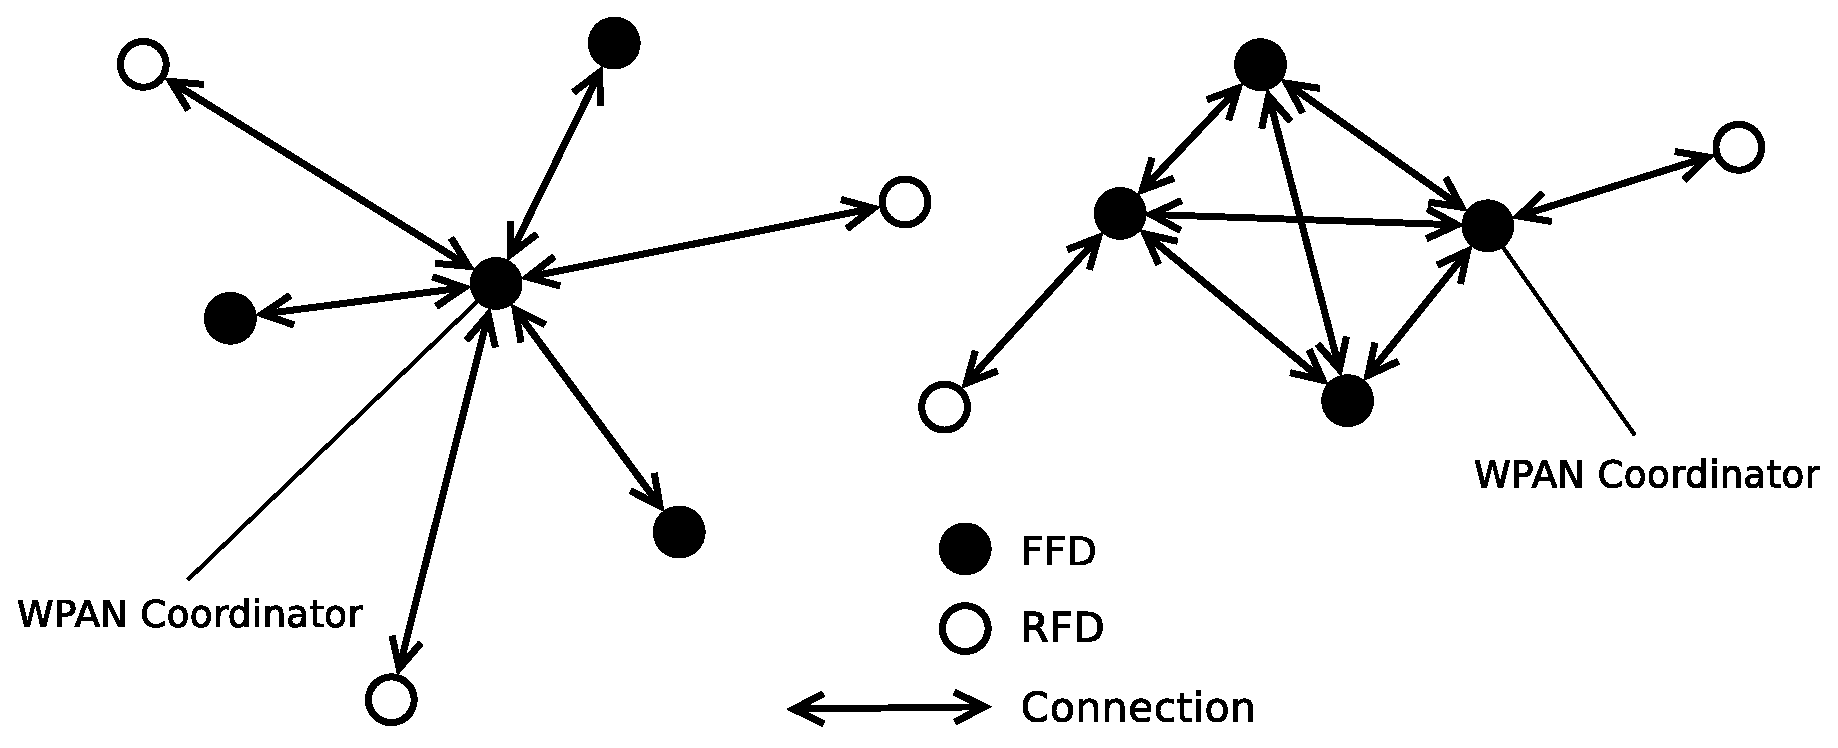
\includegraphics[width=0.9\textwidth]{WPAN_Network_Topologies.eps}
 \end{center}
 \caption{Star and peer-to-peer topology examples \cite{IEEE802.15.4-2006}}
 \label{fig:WPAN_Network_Topologies}
\end{figure}
\end{itemize}
This work will use the peer-to-peer topology as it is more flexible and scalable than the star topology. This topology is also
complexer, that is why a simpler case of peer-to-peer topology is selected, the tree topology. In this case all devices are
structured hierarchically and all of them have a father with whom they communicate, excepting the \ac{WPAN} Coordinator who is on the top of the network.

For making this topology work, a Network Layer (not provided in 802.15.4) is needed for routing purposes. To make packets as short as possible,
and only in communicaton among \acp{FFD}, short addresses (16 bits) will be used.

\section{Physic Layer}

Although for this work \ac{PHY} Layer has not as much importance as the \ac{MAC} Layer, there are some aspects that are important and 
that are good to know. This section will focus just on these aspects.

Some of the tasks developed by the \ac{PHY} Layer are:

\begin{itemize}
 \item \textbf{Switches on and off the radio transceiver.} The transceiver has three operation modes: \ac{Tx}, \ac{Rx} and sleeping. \ac{PHY}
layer must commute among these modes by \ac{MAC} layer petitions. The standard defines that the change time between \ac{Rx} and 
\ac{Tx} and vice versa must not be bigger as 12 symbols (\textit{aTurnaroundTime} = 12 symbols = 192 $\mu$s at 2.4 GHz).
 \item \textbf{Performs the \ac{ED} of the channel.} \ac{PHY} layer measures the power level of the channels in order to choose the best one
to transmit. This measurement lasts exactly 8 symbols.
 \item \textbf{Performs \ac{CCA} to check the channel.} This indicator is a part of \ac{CSMA/CA} algorithm as it will be seen later. The
\ac{CCA} is requested by the \ac{MAC} Layer and the \ac{PHY} Layer returns IDLE or BUSY depending on the channel situation. This \ac{CCA}
period lasts exactly like the \ac{ED}, 8 symbols (128 $\mu$s at 2.4 GHz).
 \item \textbf{Channel frequency selection.} As it was already commented, the 802.15.4 standard contemplates 3 different frequency 
ranges, although only the 2450 MHz will be used in this work. At this frequency, the standard stipulates 
the use of a \ac{O-QPSK} modulation with a symbol rate of 62,5 symbols/s. As this modulation makes 4 bit per symbol, we get 
a 250 Kbit/s bit rate. This frequency range has 16 different channels with a 5 MHz separation between them. The number of 
these channels goes from 11 to 26.
 \item \textbf{Data transmission and reception.} According to the standard, the \ac{PHY} Layer must be able to transmit with a minimum
power of 1 mW and it must have a sensibility of at least -85 dBm \cite{IEEE802.15.4-2006}. Figure \ref{fig:PPDU} shows the physical level frame structure.

\vspace*{1cm}

\begin{figure}[ht]
 \begin{center}
  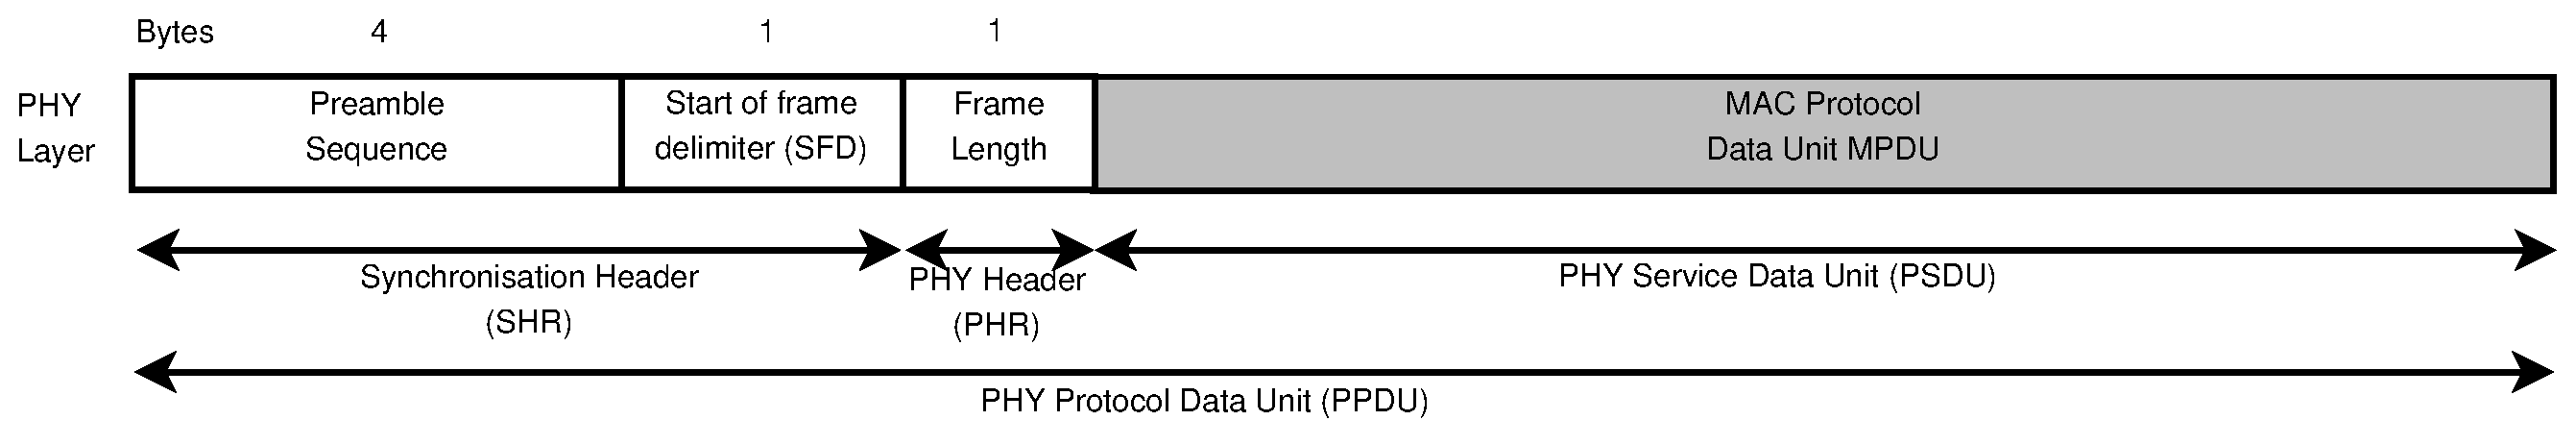
\includegraphics[width=0.9\textwidth]{PPDU.eps}
 \end{center}
 \caption{\ac{PHY} Layer frame \cite{IEEE802.15.4-2006}}
 \label{fig:PPDU}
\end{figure}
\end{itemize}

\section{\ac{MAC} Layer}

\ac{MAC} layer is responsible for connecting the node with all the other nodes in a reachable distance. Although this layer has a reduced
primitive set (26 primitives), it is really versatile and assures the minimum necessary instructions to work. Some of the responsibilities of \ac{MAC}
layer are:

\begin{itemize}
 \item Assures a reliable link between two \ac{MAC} entities.
 \item Beacon generation if device is a router.
 \item Beacon synchronization.
 \item Nodes association and dissociation.
 \item Security mechanisms.
 \item Channel access control through \ac{CSMA/CA}.
 \item Definition of \ac{GTS}.
 \item Frame validation.
 \item Duplicated received packets control.
 \item \ac{ACK} generation to assure retransmission in \ac{MAC} layer. This is a transmission protection mechanism.
\end{itemize}

As happened for the \ac{PHY} layer, the \ac{MAC} layer has some constants and attributes to be configured, which will be used later in this work.
These parameters can be found from page 133 in \cite{IEEE802.15.4-2006}.

\subsection{Working Modes}

\ac{MAC} protocol supports two working modes. The coordinator is the one responsible to choose a mode when initializing the network:

\begin{itemize}
 \item \textbf{Beaconed mode.} In this mode, the coordinator generates a beacon which is transmitted along the network thanks to the routers.
This beacon synchronizes all the devices in the network so they can sleep all the time and just wake up when they know the data will come. 
 \item \textbf{Non-Beaconed mode.} In this mode, the devices are not synchronized by beacons. For this reason, the routers and the coordinator must
be awake all the time and the end devices are the only ones that can sleep. This is not a problem, as we assumed that \ac{FFD} would be plugged 
in and only \ac{RFD} would work with batteries. Furthermore, the problem that end devices do not know when the data from the router will come, 
will be solved with the help of the proposed High Configurable Protocol.
\end{itemize}

Non-Beacon mode was selected for this work as it is more flexible for our purposes than Beaconed mode. The challenge of this choice is to 
define in Application Layer all the sleep and wake-up processes, which would have been automatically administrated in the rejected Beaconed
mode by \ac{MAC} Layer. From now on, all explanations will refer only to Non-Beaconed mode.

\subsection{\ac{CSMA/CA} Algorithm}

When \ac{MAC} Layer receives a message to be sent, before sending it, asks the \ac{PHY} Layer to check if the channel is free. In this case, it 
orders the \ac{PHY} Layer to transmit this message. The whole process is controlled by an algorithm which is called \ac{CSMA/CA}. In this 
case as a non-beaconed mode is used, the \ac{CSMA/CA} algorithm corresponds to the non-slotted one, where the random time a device waits 
before transmitting is not synchronized with the beacons. A graphic approach to this algorithm is given in Figure \ref{fig:CSMACA}, where the
processes to be commented are signaled with a number in brackets.

\begin{itemize}
 \item \textbf{(1)} - Restarts the parameters to their initial values. \ac{NB} is a counter of the number of times the process was done. \ac{BE}
is the exponent for the Backoff Random time calculation. At the beginning it takes the minimum defined by the user (\textit{macMinBE}), usually 3.
 \item \textbf{(2)} - In this step a random number between 0 and $2^{\ac{BE}}$ - 1 is generated and multiplied by the unit Backoff period, defined
by \textit{aUnitBackoffPeriod} in the standard whose default value is 20 symbols = 320 $\mu$s.
 \item \textbf{(3)} - After this waiting period while the node is in IDLE mode, \ac{MAC} orders \ac{PHY} to sense the channel performing the \ac{CCA} 
(8 symbols = 128 $\mu$s). If the channel is free, the \ac{MAC} proceeds to transmit the packet and if not, the algorithm proceeds with the 
step (4).
 \item \textbf{(4)} - If the channel was busy, first \ac{NB} and \ac{BE} are raised in one unit. Afterward, if the new \ac{BE} is bigger than the maximum
(\textit{macMaxBE}), usually 5, \ac{BE} is assigned this maximum value.
 \item \textbf{(5)} - Then maximum number of tries (\textit{macMaxCSMABackOffs}) is checked. If the maximum is not reached, the process starts again from (2),
but if it is reached, the entire process gets canceled and \ac{MAC} layer informs upper layers about the failure (\ac{CAF}).
\end{itemize}

\begin{figure}[!ht]
 \begin{center}
  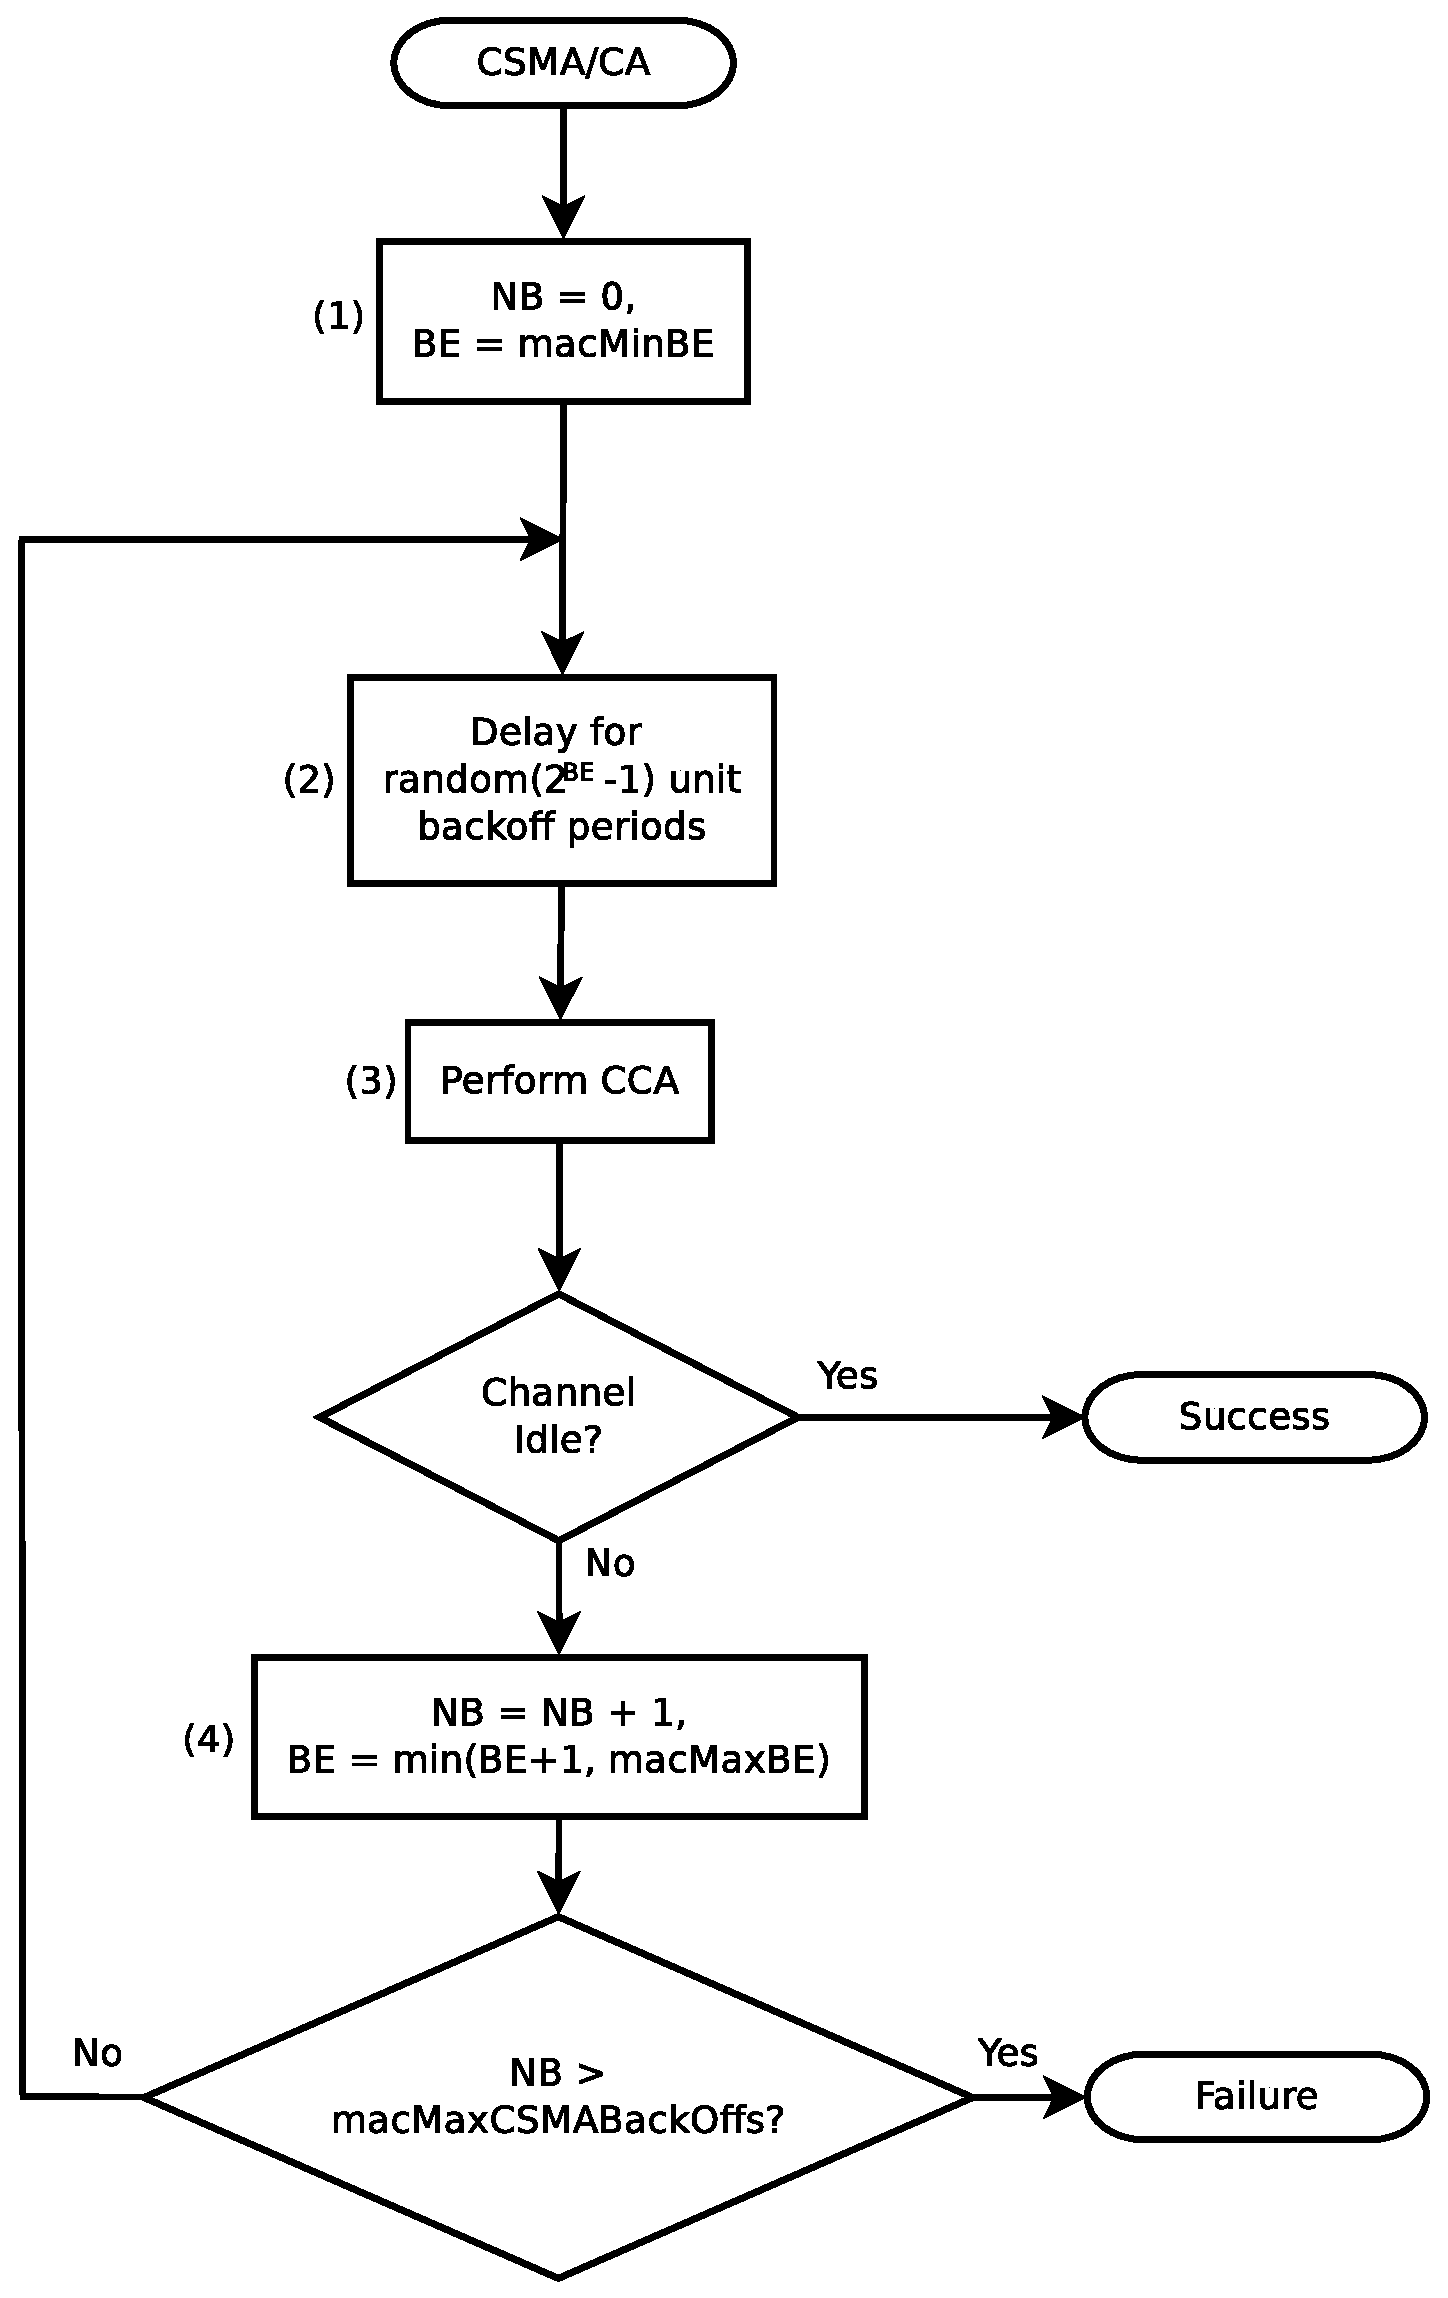
\includegraphics[width=0.5\textwidth]{CSMACA.eps}
 \end{center}
 \caption{Non-Slotted \ac{CSMA/CA} Algorithm \cite{IEEE802.15.4-2006}}
 \label{fig:CSMACA}
\end{figure}

This algorithm helps to reduce the so called collisions. These collisions could occur when a node starts transmitting without checking the 
channel, and if another node next to it has already sent some packet.

But using \ac{CSMA/CA} algorithm does not solve this problem. It could also happen that two packets have a collision in the air. One 
reason could be that while one node is performing the \ac{CCA}, another node does the same. In this case, both of them will start transmitting 
producing a collision. The other reason is the well known Hidden Terminal Problem. To explain this phenomena, Figure \ref{fig:HiddenTerminalProblem}
will be used. Node A wants to communicate with node B, but node C is already transmitting something to node B. As we can see with the dotted line,
the range of A does not cover node C. Because of this, when A performs the \ac{CCA}, it does not get any signal from C. Then node A starts transmitting, and 
node B takes at the same time a message from A and C, having a collision.

\begin{figure}[!ht]
 \begin{center}
  \includegraphics[width=0.3\textwidth]{HiddenTerminalProblem.eps}
 \end{center}
 \caption{Hidden Terminal Problem Scenario}
 \label{fig:HiddenTerminalProblem}
\end{figure}

\ac{CSMA/CA} algorithm makes also possible a situation where a node could transmit without collision but it detects a packet in the air and does
not transmit. To explain this case, Figure \ref{fig:ExposedNodeProblem} will be used. In this situation, C is already transmitting something to D and B 
wants to transmit some information to A. When B performs the \ac{CCA}, it detects the channel as busy with C to D packet. Therefore B waits another
Backoff random time and does not transmit, although it could, as its packet would have reached A and would not have disturbed D.

\begin{figure}[!ht]
 \begin{center}
  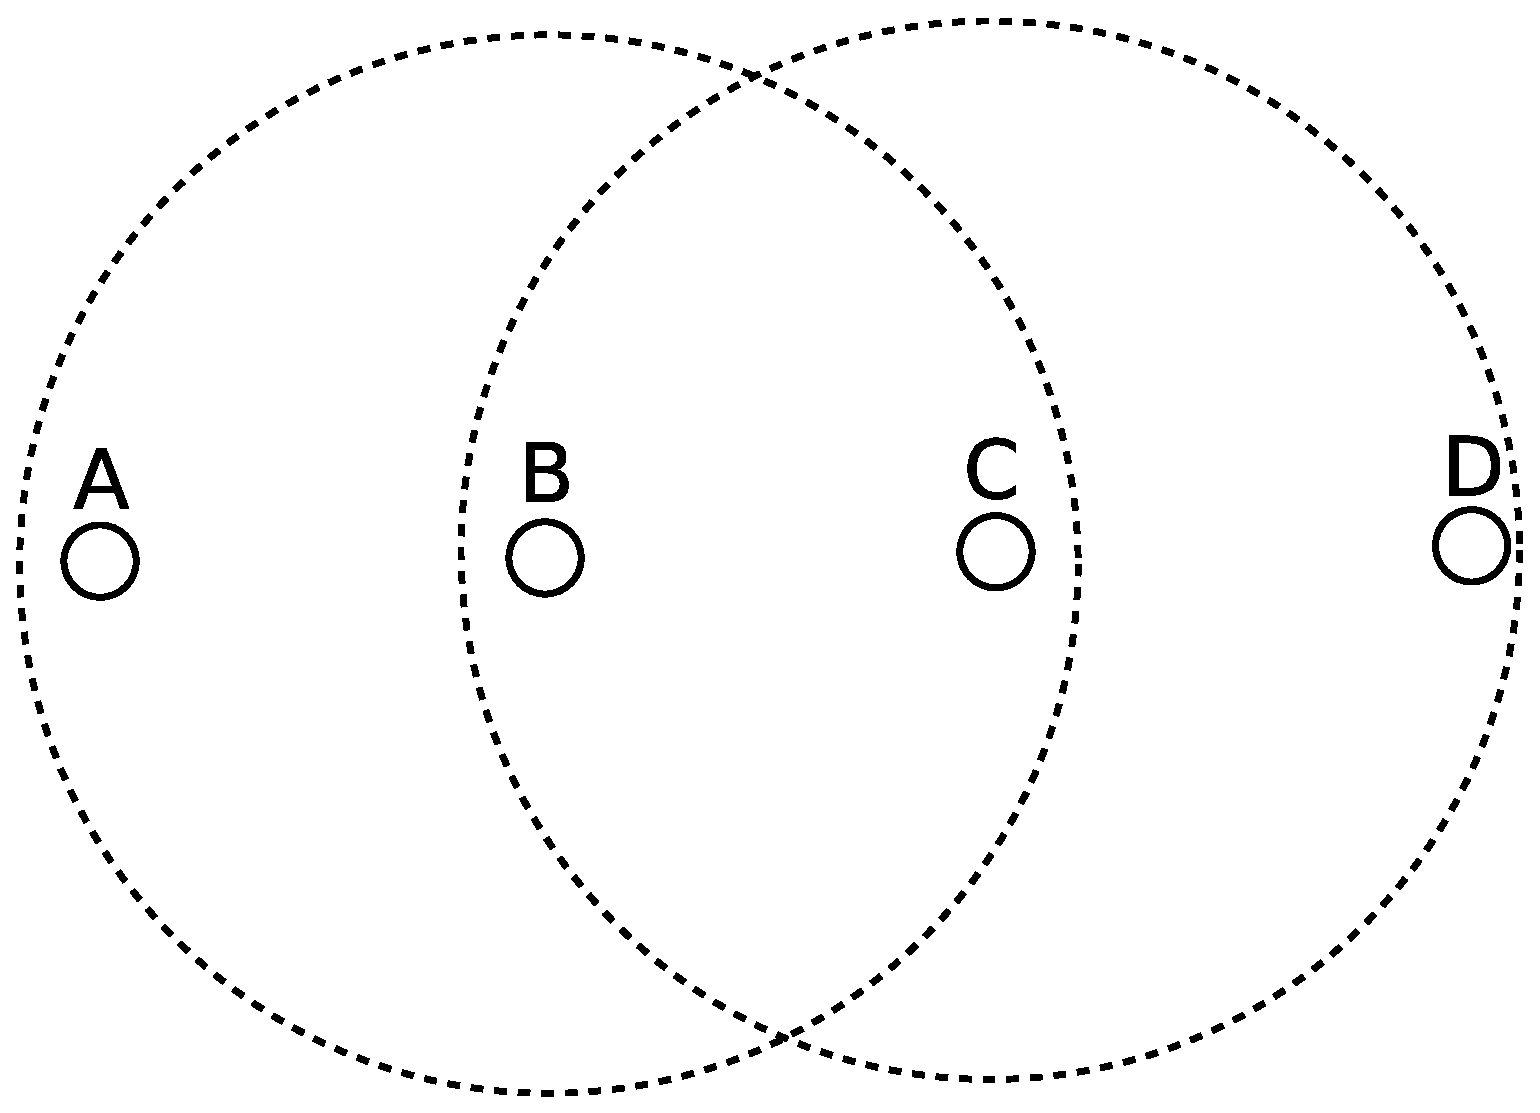
\includegraphics[width=0.3\textwidth]{ExposedNodeProblem.eps}
 \end{center}
 \caption{Exposed Node Problem Scenario}
 \label{fig:ExposedNodeProblem}
\end{figure}

Apart from the times already commented like \ac{CCA} or Backoff, there are other important times to be taken into account. \ac{SIFS} is the 
time to leave between two consecutive frames when the frame was short $(\le 18 bytes)$ and its value is 12 symbols = 192 $\mu$s. \ac{LIFS} 
is the same as \ac{SIFS} but to use with long frames (40 symbols = 640 $\mu$s). Usually these two times are included in \ac{CSMA/CA} process, 
and they are important not to collapse the system and lose data. Another important time is \textit{aTurnaroundTime}, this time is 192 $\mu$s 
and corresponds to the time needed to switch between \ac{Rx} and \ac{Tx} modes and vice versa. It is also the time to leave between the end 
of a packet reception and the start of the \ac{ACK} transmission.

\subsection{Frame Format}

\ac{MAC} packets use different frames depending if the network is beaconed or non-beaconed. As this work is using just the non-beaconed mode,
only the frames related to this mode will be explained. Figure \ref{fig:MACFrame} contains the structure that will be explained now.

\begin{figure}[!ht]
 \begin{center}
  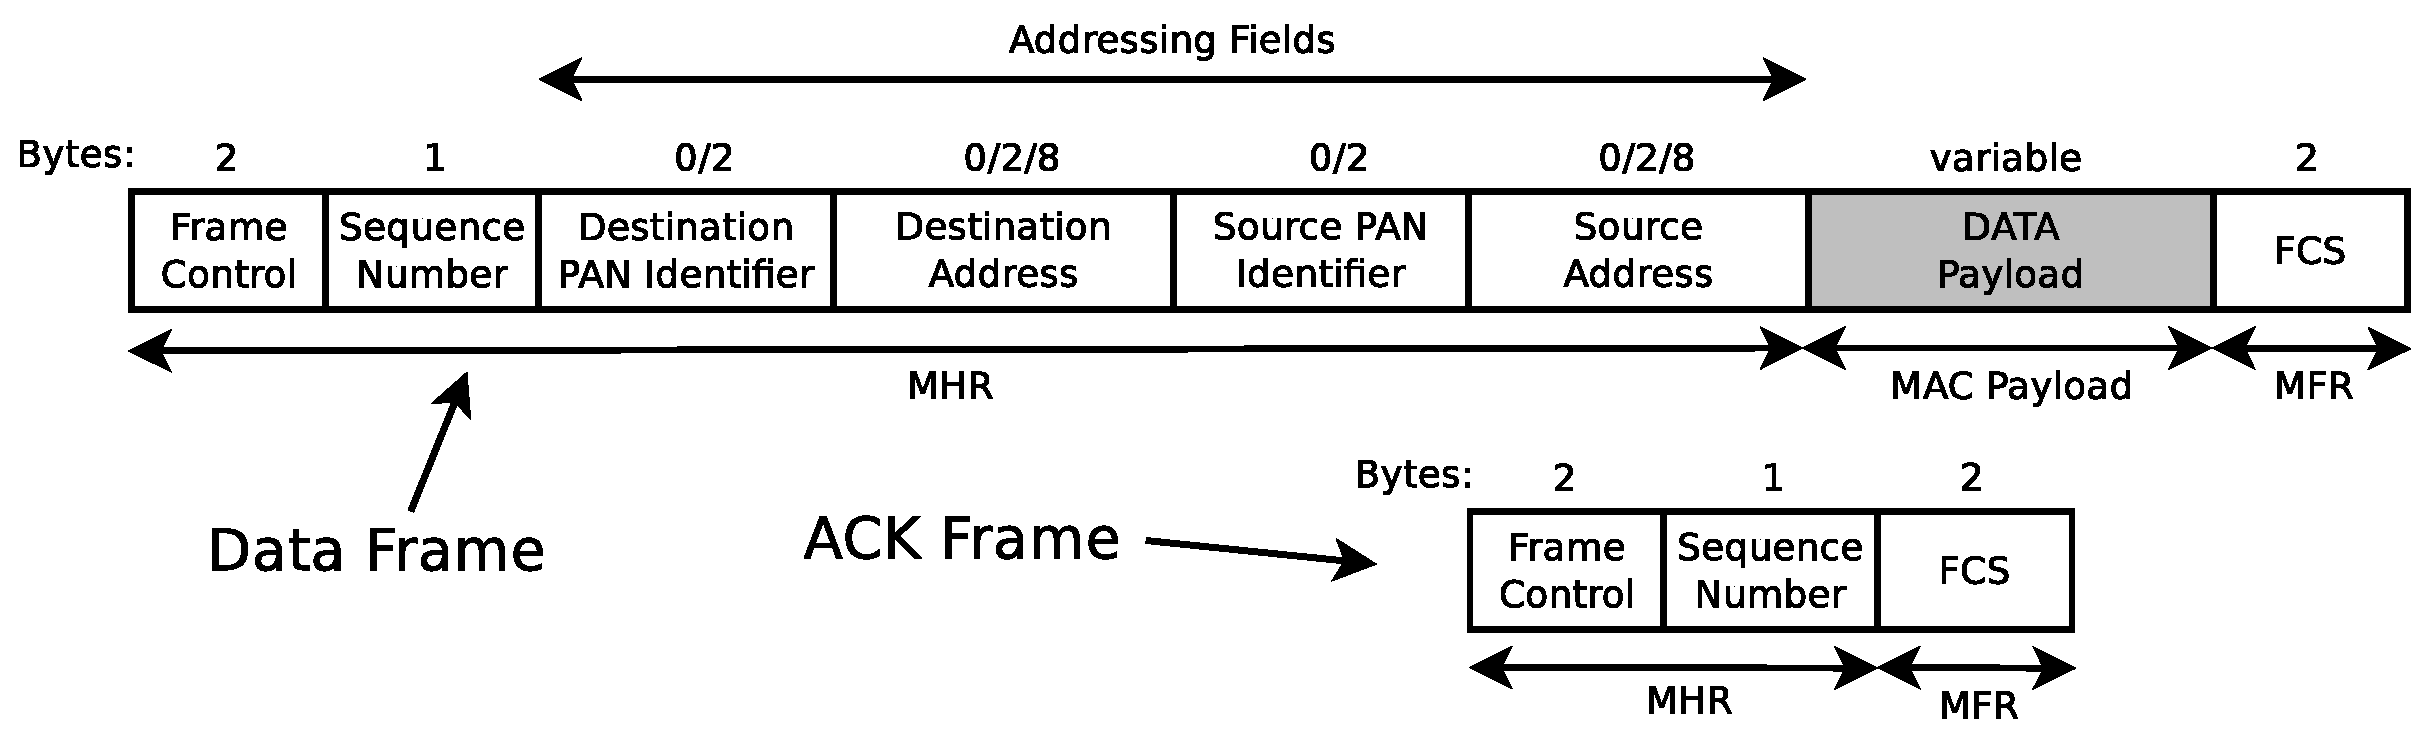
\includegraphics[width=0.7\textwidth]{MACFrame.eps}
 \end{center}
 \caption{Data and \ac{ACK} \ac{MAC} Frames \cite{IEEE802.15.4-2006}}
 \label{fig:MACFrame}
\end{figure}

\begin{itemize}
 \item \textbf{Header (\ac{MHR}).} Formed by:
  \begin{itemize}
   \item Frame Control: 16 bits to define the frame type, security code, \ac{ACK} required, etc.
   \item Sequence Number: 8 bits to identify the frame.
   \item Destination \ac{PAN} Identifier: 16 bits to indicate the \ac{PAN} communicating with. 0xFFFF if any network is selected.
   \item Destination Address: 16 or 64 bits depending if it is a short or long address. End devices use always a long address and routers a short one.
   \item Source PAN Identifier: 16 bits to indicate the source \ac{PAN}.
   \item Source Address: 16 or 64 bits depending if it is a short or long address, end devices use always long address and routers short.
  \end{itemize}
 \item \textbf{Payload.} Data from upper layer.
 \item \textbf{\ac{MFR}.} 16 bit sequence known as \ac{FCS}, this is a \ac{CRC}.
\end{itemize}

\subsection{Hardware}

Although this work is based on a simulation, all the needed physical parameters to simulate are obtained from the commercial hardware 
RCB230 V3.2 as it is the one available in the department. This node has a AT86RF230 transceiver and a ATmega1281V \ac{uC}. According 
to \cite{LPLandOLP}, the consumption values of this node are the ones shown in Table \ref{tab:NodeEnergyConsumption}. Transition times that are not defined
in 802.15.4 standard are in Table \ref{tab:NodeTiming}.


\begin{table}
 \begin{center}
  \begin{tabular}{|l|c|}
   %\noalign{\vspace*{0.5cm}}
   \hline
   & \textbf{Energy Consumption} \\
   \hline
   Transceiver \ac{Rx} mode & 0.06496 mW/s \\
   \hline 
   Transceiver \ac{Tx} mode & 0.06672 mW/s \\
   \hline
   Transceiver IDLE mode & 0.04342 mW/s \\
   \hline
   Transceiver Sleep mode & 0.0728 $\mu$W/s \\
   \hline
   \ac{uC} (Transceiver Sleeps) & 0.03042 mW/s \\
   \hline
  \end{tabular}
  \caption{Node RCB230 V3.2 Energy Consumption \cite{LPLandOLP}}
  \label{tab:NodeEnergyConsumption}
 \end{center}
\end{table}
\begin{table}
 \begin{center}
  \begin{tabular}{|l|c|}
   %\noalign{\vspace*{0.5cm}}
   \hline
   & \textbf{Transition timing} \\
   \hline
   Transition: Sleep -> \ac{Rx} & 1.88 ms \\
   \hline 
   Transition: \ac{Tx} -> Sleep & 0.94 ms \\
   \hline
   Transition: \ac{Rx} -> Sleep & 0.94 ms \\
   \hline
  \end{tabular}
  \caption{Transceiver AT86RF230 transition timing \cite{LPLandOLP}}
  \label{tab:NodeTiming}
 \end{center}
\end{table}


\chapter{Protocol Design}
\label{chap:protocoldesign}

In the state of the art, there are different protocols constructed over \ac{IEEE} 802.15.4, like ZigBee, WirelessHART, 6LoWPAN \ldots \ some
are prepared for low consumption, others build different applications, but almost none of them are focused in localization. In the
department \ac{LPL} and \ac{OLP} \cite{LPLandOLP} protocols were proposed for this purpose. This protocols are based in \ac{IEEE} 802.15.4 and specifically 
designed for localization. In the next section a brief overview will be given, for a deeper view, please consult \cite{LPLandOLP}.

\section{\ac{LPL} and \ac{OLP}}

\ac{LPL} and \ac{OLP} \cite{LPLandOLP}, are two protocols designed for localization and based in \ac{RSSI} values. This values give an idea of 
the received signal strength in the device, and have the advantage that this information is already in all packets a device receives, there
is no need of special hardware or data to be prepared or obtained like in other methods (ultra wide band for example). But \ac{RSSI} values have 
a big problem for localization, its dispersion is very big, making the localization resolution (in some cases up to many meters 
\cite{fingerprint}) bad for some applications. 

This resolution problem, can be solved through some approaches. One kind is using localization techniques like ``fingerprint 
technique'' \cite{fingerprint} that improves the resolution. Another option is, taking more than 1 \ac{RSSI} value to obtain a more stable 
result. This technique has one big challenge, the more values are taken, the higher the energy consumption. Without a good approach, 
the \ac{MN} would need to listen to the channel most of the time waiting to receive packets from \ac{AN} to obtain \ac{RSSI} values, 
this way a lot of energy would be wasted just doing nothing, this is called idle listening. This 2 protocols propose 2 different 
approaches to solve this.

Another aspect in localization is who calculates the position, 3 different alternatives can be obtained.

\begin{itemize}
 \item \textbf{Centralized.} A central computer receives the \ac{RSSI} values from all \acp{AN} in the network and calculates the positions of 
the \acp{MN}. The advantage is that the computer can use complicate algorithms to obtain better results, but this method 
charges the network with a lot of traffic, specially if the \ac{MN} needs to know its position back after calculation.
 \item \textbf{Distributed-A.} The \ac{MN} sends the \ac{RSSI} values directly to the \ac{AN}, and this calculates directly the \ac{MN} position,
this does not charge the network so much like the centralized approach but the resolution is also not so good. It is important to note that 
each \ac{MN} has a ``selected \ac{AN}'', this \ac{AN} is the one in charge to calculate \ac{MN} position and the one the \ac{MN} communicates
with and through. This \ac{AN} is usually the one closest to the \ac{MN}.
 \item \textbf{Distributed-M.} In this mode, is the \ac{MN} who calculates directly its position from \ac{RSSI} values obtained from \acp{AN},
the problem is that \acp{MN} cannot use powerful localization algorithms. This solution is the one that almost does not charge the network.
\end{itemize}

The protocols \ac{LPL} and \ac{OLP} are going to use phases for different behaviors, and this phases will be repeated cyclically, that's why 
a good synchronization among all the nodes is necessary so all nodes can start the phases at the same time. Nodes will get 
the synchronization information from their parents (do not forget that a tree topology is used) using an active or a passive synchronization. 
To get a graphical explanation check Figure \ref{fig:synchronization}.

\begin{itemize}
 \item \textbf{Passive Synchronization.} The parent starts the process sending a packet R1 to \ac{MAC} to be transmitted, this packet is
created at the time-stamp Tx1, and includes this time, the time until the next phase start (TF) and info about this phase. Due to random time in 
\ac{CSMA/CA} process and other processing times, R1 is not transmitted immediately but in Tx2. When the packet is transmitted, \ac{MAC} informs
the application layer and this creates another packet (R2) including the new time-stamp Tx2. At the child, 2 packets will be received, R1 and 
R2 in times Rx1 and Rx2 respectively. Calculation of next phase start from the child point of view (TZ) is done like in (\ref{mat:pasivesync}).

\begin{equation}
  TZ = TF - (Rx2 - Rx1) - (Tx2 - Tx1)
  \label{mat:pasivesync}
\end{equation}

\begin{figure}[here]
 \begin{center}
  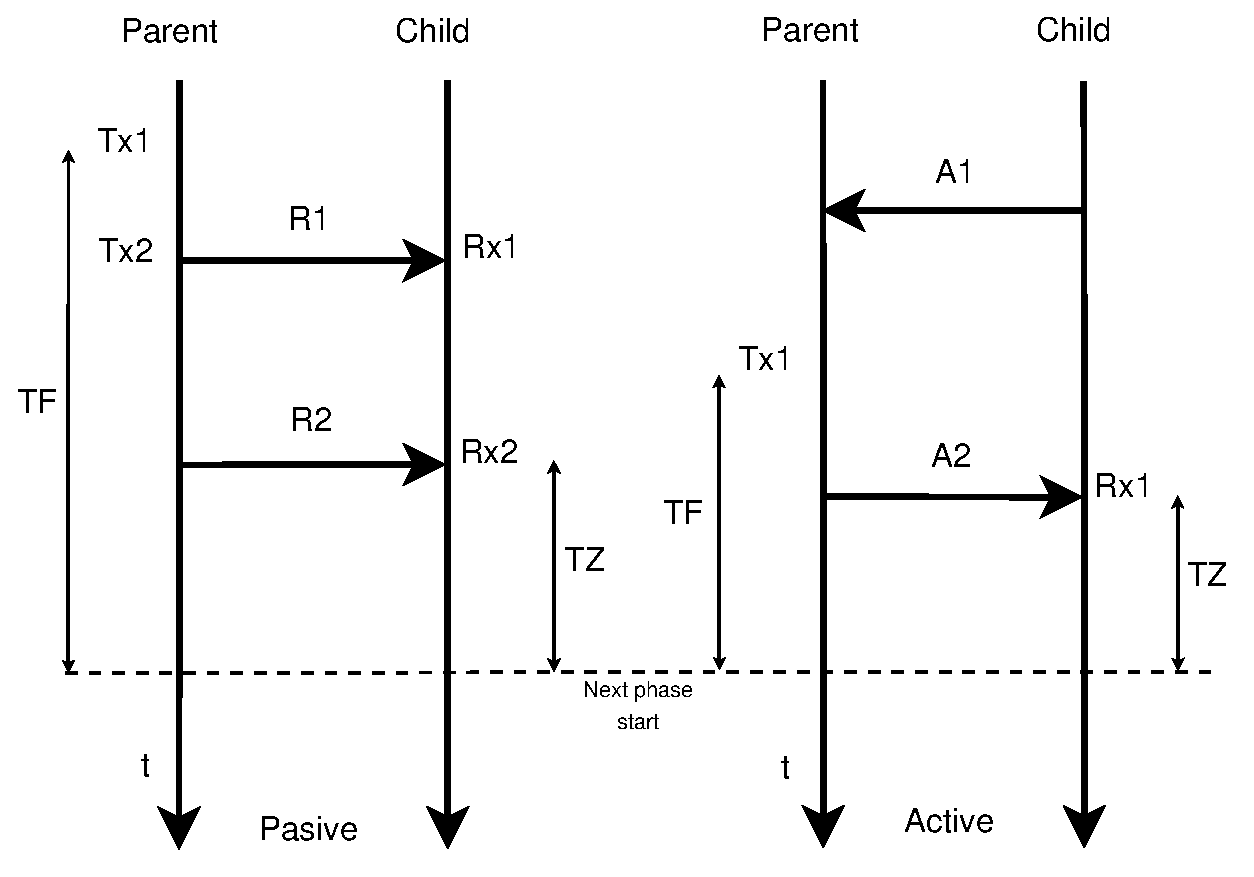
\includegraphics[width=0.6\textwidth]{synchronization.eps}
 \end{center}
 \caption{Passive and Active Synchronization \cite{LPLandOLP}}
 \label{fig:synchronization}
\end{figure}
 
 \item \textbf{Active Synchronization.} In the active synchronization, the child starts the process sending a synchronization request (A1),
then the parent answers with packet A2, this packet contains the time until the start of the next phase (TF). The child can calculate this time
with like in (\ref{mat:activesync}).

\begin{equation}
  TZ = TF - C
 \label{mat:activesync}
\end{equation}

The C parameter in (\ref{mat:activesync}), represents an estimation of all the processing times and random times from \ac{CSMA/CA}, that is why
this method is not so exact like the passive one, although it does not need 2 packets like it.
\end{itemize}

In the following subsections, both protocols \ac{LPL} and \ac {OLP} are going to be introduced.

\subsection{\acl{LPL}}

To reduce the idle listening, and thus the energy consumption, this protocol, proposes that instead of listening to the \acp{AN}, the
\acp{MN} are the ones who transmit and the \acp{AN} the ones who listen and transmit this information. This protocol is divided in 3 
phases which can be appreciated in Figure \ref{fig:LPL}.

\begin{figure}[h]
 \begin{center}
  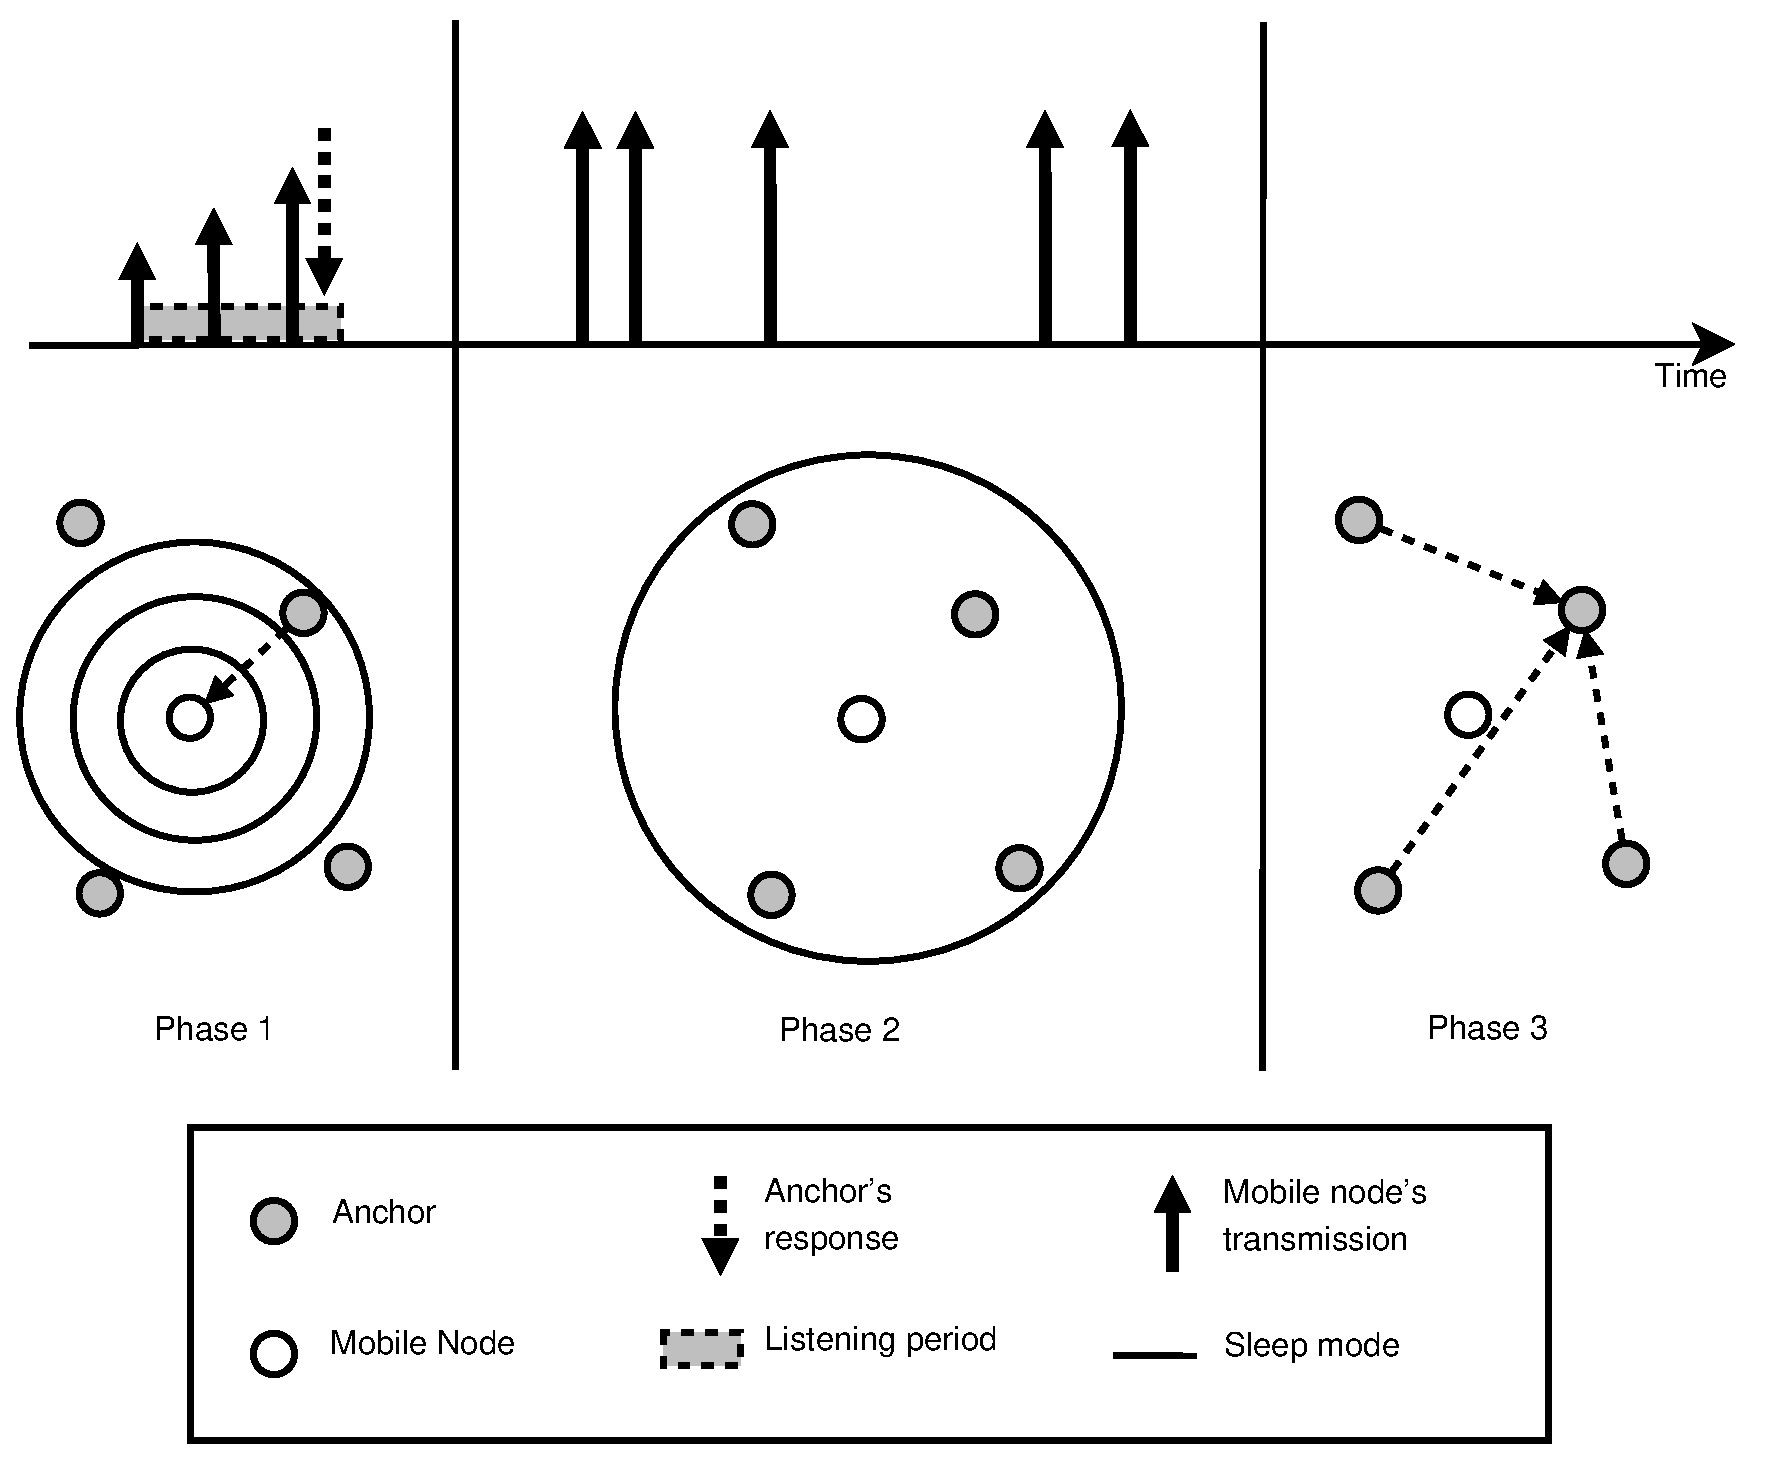
\includegraphics[width=0.7\textwidth]{LPL.eps}
 \end{center}
 \caption{LPL Phases \cite{LPLandOLP}}
 \label{fig:LPL}
\end{figure}

\begin{itemize}
 \item \textbf{Phase 1:} In this phase, \ac{MN} selects a random time to broadcast a synchronization request, starting with the minimum power,
and increasing this power until it receives an answer from an \ac{AN}, this will be the selected \ac{AN}, and the answer will contain information
about the phase times. This process makes sure that only the nearest \acp{AN} answer to this synchronization request. In the next phase 1, if 
the \ac{MN} needs to know its position, it asks its selected \ac{AN} about this information, and if not it just synchronizes.
 \item \textbf{Phase 2:} In phase 2, the \ac{MN} broadcasts several packets in random times to minimize the collisions. Any time the node is not
transmitting, it goes to sleep, this makes that \acp{MN} are awake only when they transmit eliminating this way the idle listening. The \acp{AN} that
received this broadcasts, store the read \ac{RSSI} values and the selected \ac{AN}.
 \item \textbf{Phase 3:} During this phase, the \acp{MN} sleeps and the \acp{AN} send the measured \ac{RSSI} values to the selected \ac{AN}. 
This \ac{AN} will calculate the \ac{MN} position in Distributed-A case or send the data to a central computer in Centralized case. In this phase is
also done the synchronization between \acp{AN} and network configuration.

This protocol, has some problems that make it not suitable for all conditions:

\begin{itemize}
 \item Hidden Terminal Problem. This problem is here strong not only because it could make big idle listening in phase 2, but it could also 
happen that, if 2 \acp{MN} transmit at the same time, the selected \ac{AN} might not be the one closest to the \ac{MN} but one with a not so 
good connection.
 \item High \ac{MN} number. If the number of \acp{MN} is high, phase 2 is going to be full of collisions and thus, the idle listening will be
high. In phase 1, the hidden terminal problem would be stronger.
 \item Selected \ac{AN} selection. If many \acp{AN} are close to the \ac{MN}, all of them are going to try to answer causing collisions. Also, 
when the \acp{AN} are not close to the \ac{MN}, a lot of energy is wasted in the \ac{MN} trying to detect gradually the selected \ac{AN}.
\end{itemize}


\end{itemize}


\subsection{\acl{OLP}}

In the case of \ac{OLP} protocol and unlike \ac{LPL}, the \ac{MN} is the one who listens. This protocol is also divided in 3 phases, 2 of 
them can be appreciated in Figure \ref{fig:OLP}.

\begin{figure}[ht]
 \begin{center}
  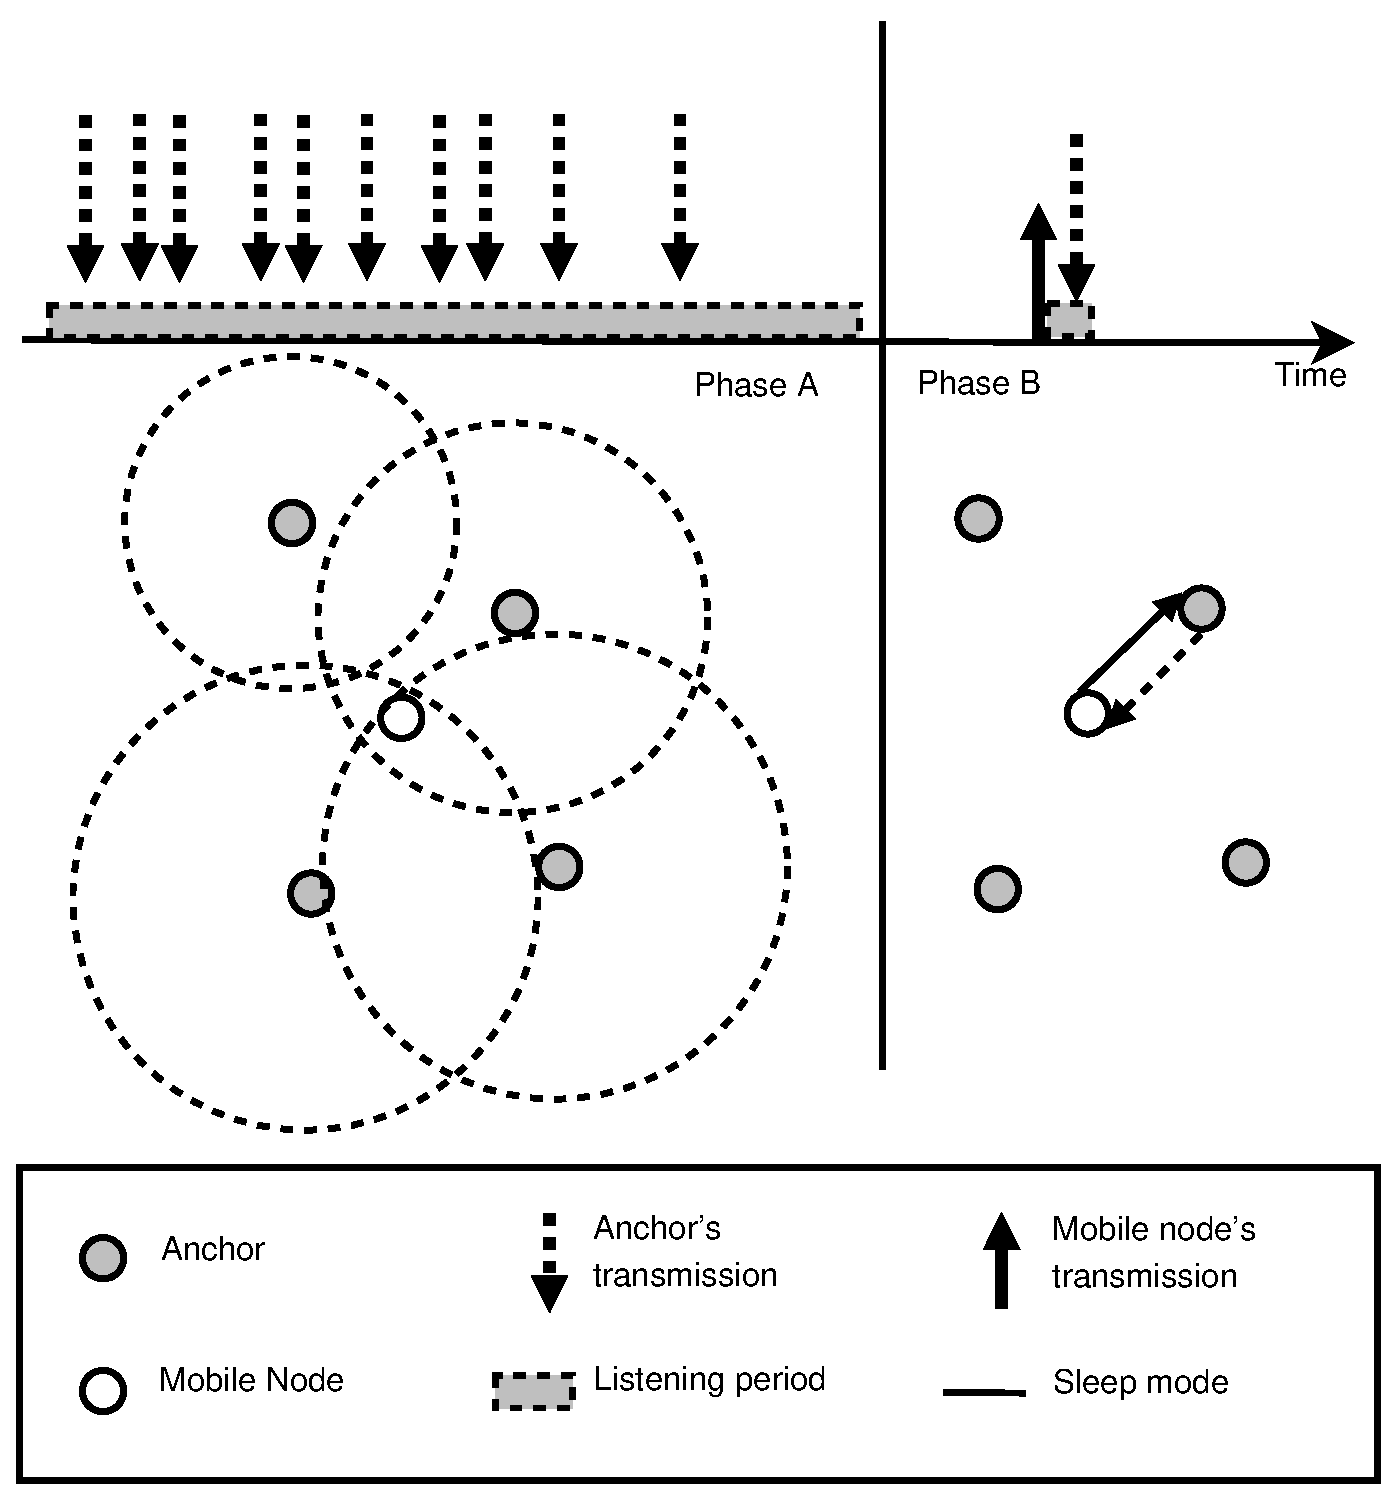
\includegraphics[width=0.55\textwidth]{OLP.eps}
 \end{center}
 \caption{OLP Phases \cite{LPLandOLP}}
 \label{fig:OLP}
\end{figure}

\begin{itemize}
 \item \textbf{Phase A:} In this phase, and thanks to the synchronization among \acp{AN}, the inter-arrival time is reduced, reducing so the
idle listening. This packets also content synchronization information for the \ac{MN}. In this phase \ac{RSSI} values are received and stored
by the \ac{MN}, and then it goes to sleep.
 \item \textbf{Phase B:} In this phase and in Distributed-M mode, the \ac{MN} will use easy localization algorithms together with all the \ac{RSSI}
values read to get its position. In case of Distributed-A or Centralized mode, the \ac{MN} will send a report to the selected \ac{AN}, took 
from the highest \ac{RSSI} value, with all the stored \ac{RSSI} values in Phase A. The selected \ac{AN} will answer with an \ac{ACK}. In next
phase B, the \ac{MN} will ask the selected \ac{AN} about its position in case it needs it.
 \item \textbf{Phase C:} Like in \ac{LPL} this Phase is reserved for communication among \acp{AN} and network configuration.
\end{itemize}

\ac{OLP} has also some problems:

\begin{itemize}
 \item Synchronization. In this protocol, a really good \acp{AN} synchronization is needed to make the idle listening in phase 1 from the 
\acp{MN} as low as possible. This is not easy, specially with a tree structure where the synchronization error will be increased and 
propagated through the tree.
 \item \ac{MN} listens too much. The \ac{MN} is listening during long periods of time where all the \acp{AN} are transmitting, some times it
could even happen that the \ac{MN} it is not at a reachable distance from the \ac{AN} that is transmitting, listening in this moment just 
for nothing.
 \item Hidden Terminal Problem. If the \acp{AN} are not good synchronized to avoid this problem, the \acp{MN} would get many invalid 
packets, being this a waste of energy. If the number of \acp{MN} is big, then in phase 2 we could have many collision problems.
 \item Temporal \ac{RSSI} Correlation. As the \ac{RSSI} values are very correlated in near times \cite{RSSIcorrelated}, receiving all 
the packets so close in time would not contribute to have a better and more stable \ac{RSSI} measurement.
\end{itemize}
 

\section{High Configurable Protocol proposal}

From the previous section and according to the results in \cite{LPLandOLP}:
\begin{quote}
``LPL consumes lower energy than OLP when many RSSI samples are required from many ANs. On the other hand,
OLP becomes more energy efficient than LPL when there are several MNs and few RSSI samples are needed.''\cite{LPLandOLP}
\end{quote}

From this, it could be extracted that depending on the application, and the network load, it could be better that some nodes could have a 
configuration where their main action is listening and others could have a configuration where their main action is broadcasting. This 
configuration should be variable depending on the current network situation and the necessities of the node. From this, arises the necessity
of a High Configurable Protocol with different node configurations.

\subsection{Node Configurations}

From the Table \ref{tab:wsn_applications} (page~\pageref{tab:wsn_applications}) where different applications for \ac{WSN} where stated and the
previous paragraph, it is possible to extract this 4 different node configurations.

\begin{itemize}
 \item \textbf{Mode 1.} This is the normal configuration, when the \ac{MN} does not have any special need. A \ac{MN} with this configuration,
will listen to the \acp{AN} and then send the selected \ac{AN} a packet with the measurements. This is equivalent to having just \ac{OLP}. This
configuration supports the Centralized and Distributed-A working modes.
 \item \textbf{Mode 2.} This configuration mode is similar to mode 1, but in this case is prepared to work only with Distributed-M working mode.
From time to time in case it's needed, it could send the estimated positions to its selected \ac{AN}.
 \item \textbf{Mode 3.} This configuration, also called \ac{VIP} mode, is used when the node is in a critical situation respecting the battery.
This configuration is similar to \ac{LPL} where the \ac{MN} broadcasts and the \acp{AN} receive the packets and send them to a coordinator that
will be able to estimate \ac{MN} position. When it is needed, a way for the \ac{MN} to request its position is provided, this will be explained 
later. 
 \item \textbf{Mode 4.} Unlike the previous configuration, this configuration is for nodes without battery problems, and with a high accuracy
need or a big urgency. This configuration is a mix of mode 1 and 3, the \ac{MN} listens to the \acp{AN} broadcasts but also they broadcast their
self packets to be measured by the \acp{AN}, all this information together is sent to a coordinator that will estimate \ac{MN} position.
This node loads the network so much and will be used just when strictly needed.
\end{itemize}

This is just a brief description of the different configurations. As the protocol is yet to be explained, a full behavior description from 
every configuration will be done later together with the protocol description.

\subsection{Protocol Description}

From previous section, it is obtained that this protocol, needs at least 3 different phases to work. One of the phases is Sync 
Phase, where the \acp{AN} will transmit broadcasts and the \acp{MN} will listen to get \ac{RSSI} values and synchronize. Another needed 
phase is a phase where \acp{AN} and \acp{MN} could communicate among them. And the last needed phase, is a phase where the \acp{AN} could 
communicate with each other to and from the coordinator.

\acp{MN} configured with mode 3, are nodes with critical battery. This nodes cannot waste energy, and this means their idle listening must be
as low as possible. As this nodes will not waste time listening and will just transmit broadcasts, it could be interesting reserving a phase
just for them, where their transmissions will not interfere with the ones from the rest of the \acp{MN}, this phase will be called \ac{VIP} 
Phase. It is clear, that the number of \ac{VIP} \acp{MN} cannot be too big as this way, their exclusivity will not be anymore exclusive.
This phase should not be so long as there are still many other \acp{MN} to transmit and the phases collection would become too long.
The phase for communication among \acp{MN} and \acp{AN} will be named Report Phase, and here is where Mode 4 \acp{MN} can make 
their broadcasts and where communication among \acp{MN} and \acp{AN} can take place.

The main purpose of the phase where \acp{AN} communicate with each other, is to transmit information between the coordinator or sink and 
the \acp{MN}. That is the reason why this phase will be called ComSink Phase. This phase should be the biggest one, as all traffic from 
the \acp{MN} should reach the sink and come back, and all \acp{AN} must transmit their own \acp{MN} information and route the one coming from
their sons or parents. As the traffic in this phase will be high, its useful to distinguish between up-links traffic and down-links traffic, 
ComSink Phase will be divided in ConSink Phase 1 (up-links) and ComSink Phase 2 (down-links).

As it was said, \ac{RSSI} values are very correlated in near times \cite{RSSIcorrelated}, that is why it could be favorable to distribute the 
Sync Phase to get better \ac{RSSI} samples. As apart from Sync Phase, the protocol consists in Report Phase, \ac{VIP}
Phase, ComSink Phase 1 and ComSink Phase 2, if Report Phase and \ac{VIP} Phase are scheduled together, Sync Phase can be divided into 3
separated in time phases, Sync Phase 1, Sync Phase 2 and Sync Phase 3. This sync phases will be intercalated between the other phases.

This phase collection will be repeated in time, being the period every phases collection repetition. For a better understanding of this 
phase division, check Figure \ref{fig:ProtocolPhases}. This Figure will be explained in detail later.

\begin{figure}[ht]
 \begin{center}
  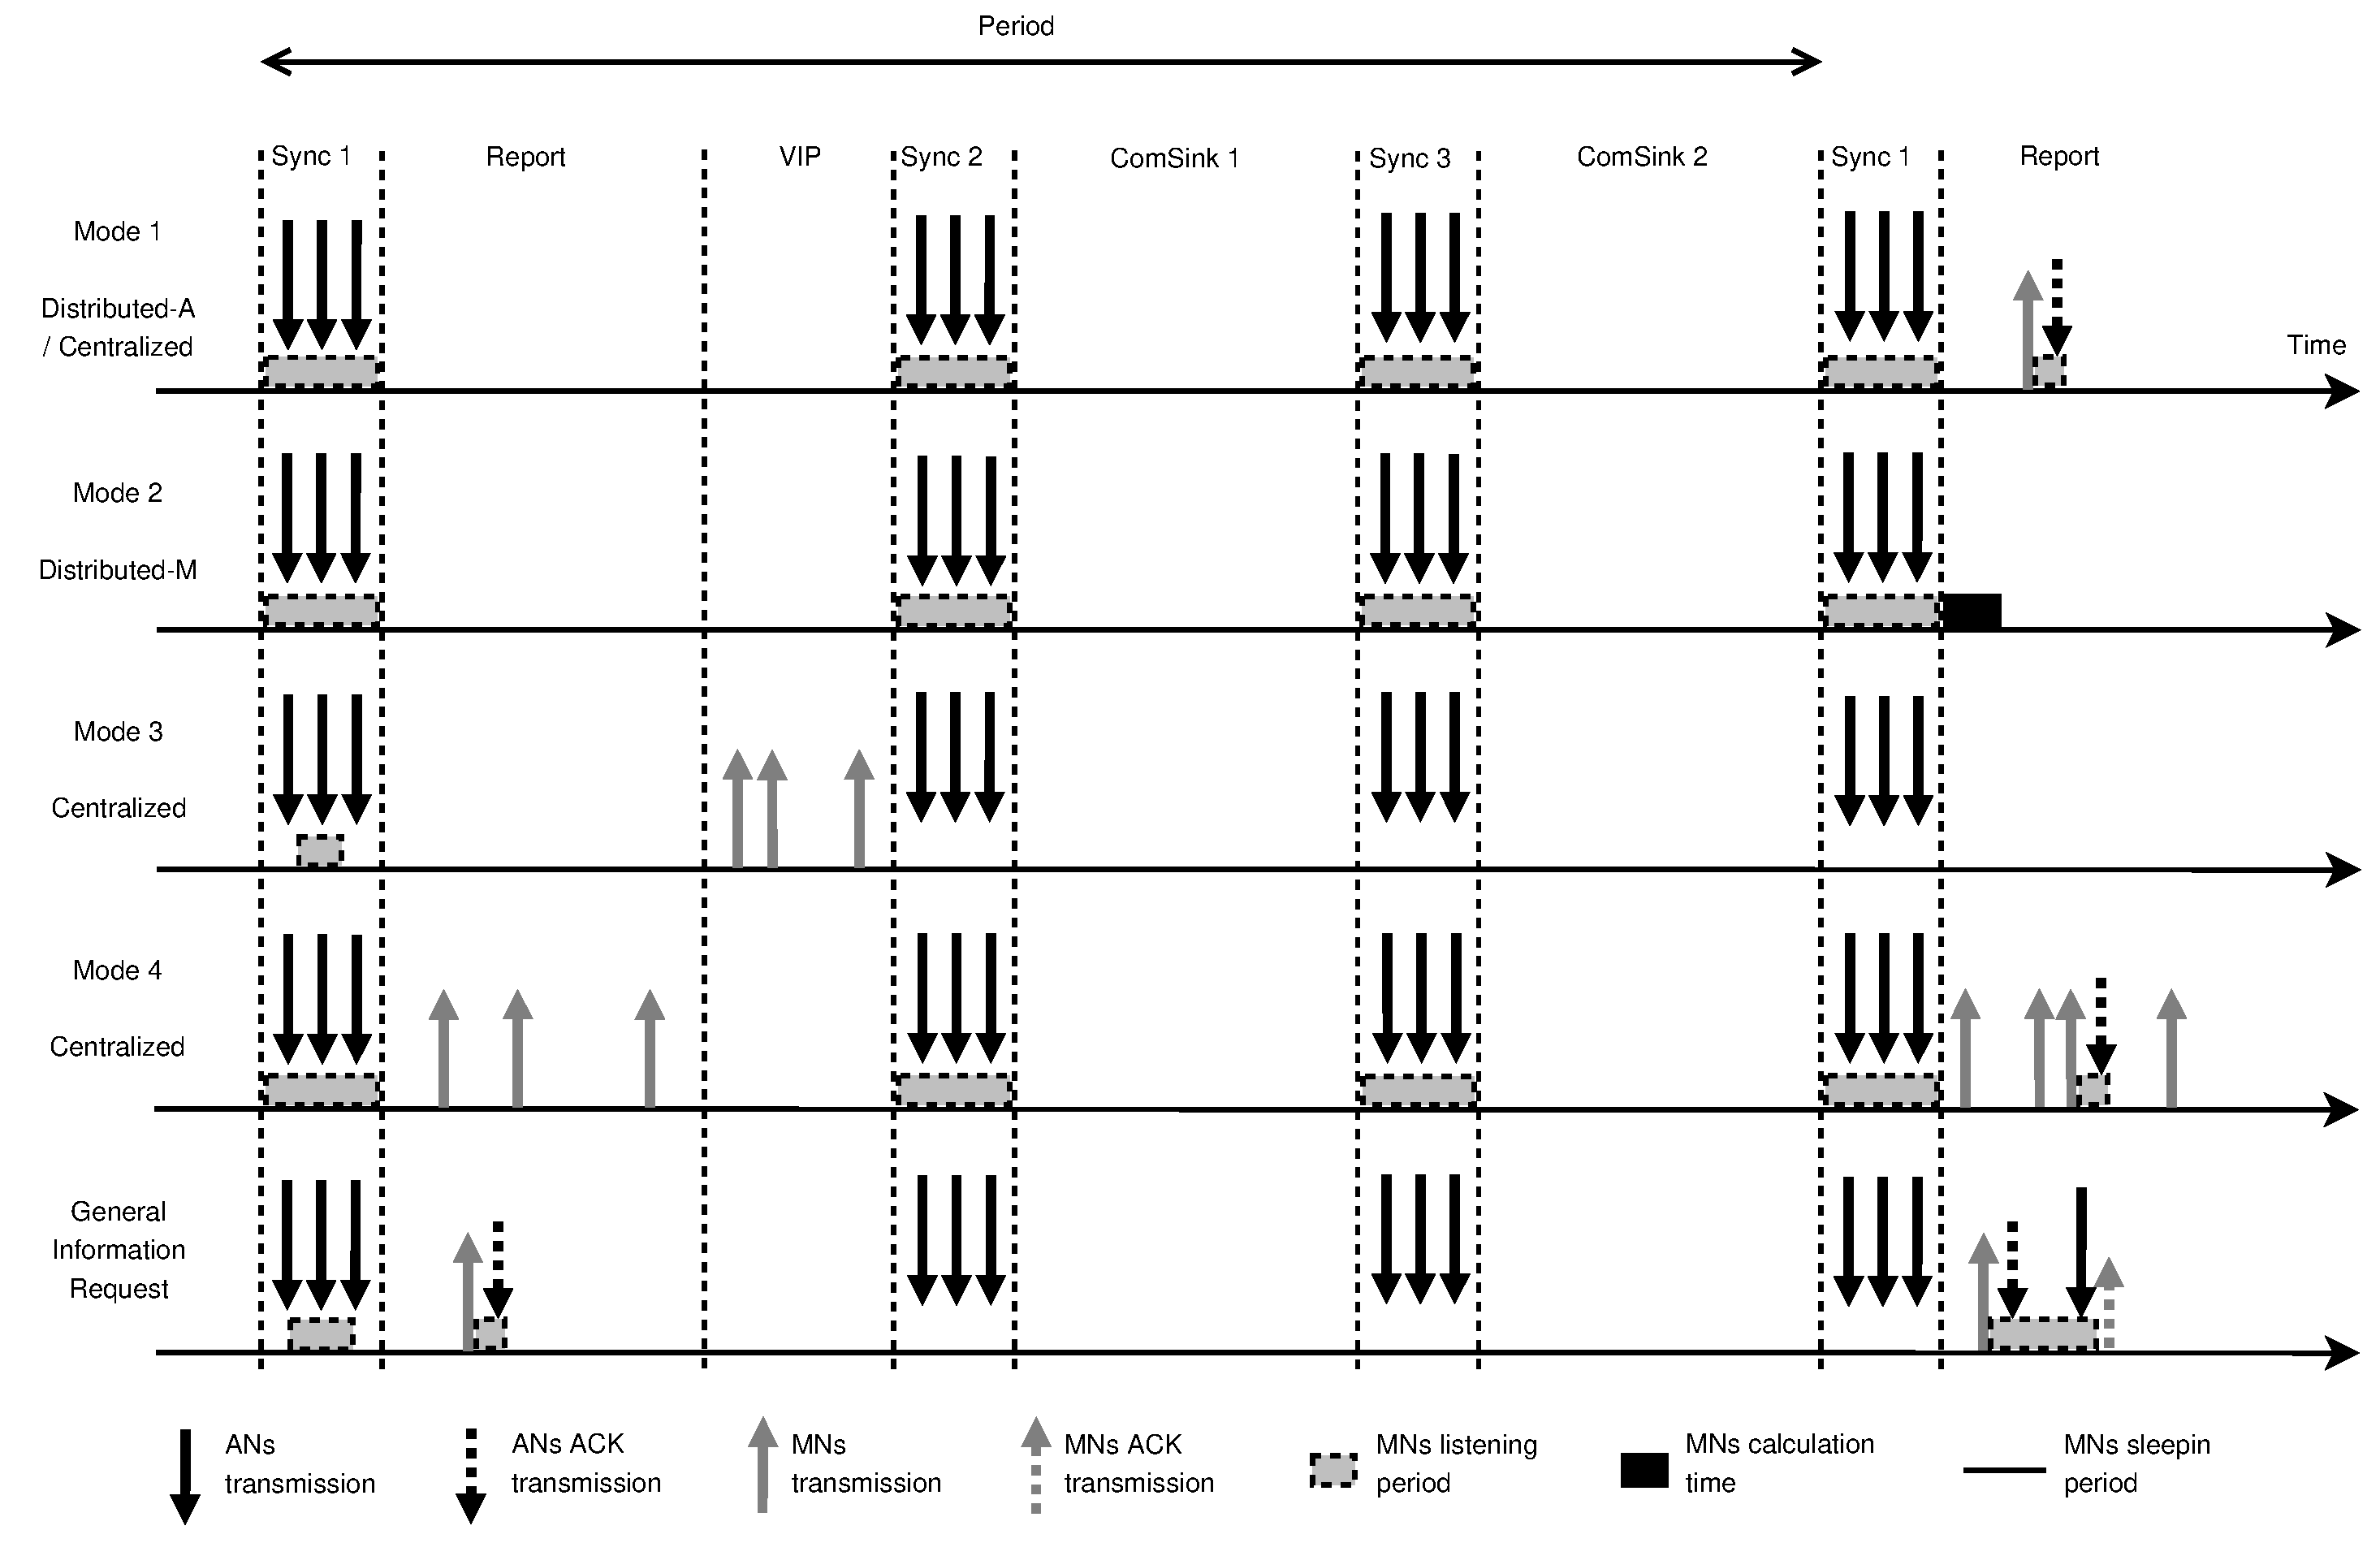
\includegraphics[width=1\textwidth]{ProtocolPhases.eps}
 \end{center}
 \caption{High Configurable Protocol Phases \cite{mipaper}}
 \label{fig:ProtocolPhases}
\end{figure}

The Figure \ref{fig:ProtocolPhases} is divided into 5 sections, one per Configuration Mode and the last one for explaining the General Information
Request. To understand properly how the protocol works, this sections have to be explained in detail:

\begin{itemize}
 \item \textbf{Mode 1.} This \acp{MN} listen during the Sync Phases to the \acp{AN} broadcasts, here they take the \ac{RSSI} values and send them
to their selected \ac{AN}, this is obtained from the highest measured \ac{RSSI}. The selected \ac{AN} answers with an \ac{ACK} to the \ac{MN}.
 \item \textbf{Mode 2.} 
 \item \textbf{Mode 3.} 
 \item \textbf{Mode 4.} 
 \item \textbf{General Information Request.} 
\end{itemize}

Here, it is just defined the standard behavior of the different configurations, but to really extract a high configuration of the protocol, some 
parameters must be taken into account.

\begin{itemize}
 \item \textbf{activePhases -} This are the periods where the \ac{MN} is active with its standard behavior (already commented).
 \item \textbf{inactivePhases -} This are the periods where the \ac{MN} is sleeping.
 \item \textbf{offsetPhases -} This are the periods to leave inactive before the first active period comes.
 \item \textbf{offsetSyncPhases -} This are the Sync Phases where \acp{MN} don't listen in the first active phase, will be explained later.
 \item \textbf{reportPhases -} This is the periods frequency where the \ac{MN} can send an extra report to the \ac{AN}, even if it is 
an inactive period.
 \item \textbf{askFrequency -} This is the extra report frequency when a flag will be activated in the extra report from a \ac{MN} to 
an \ac{AN}, to indicate the \ac{AN} that next phase some information will be requested.
 \item \textbf{offsetReportPhases -} This are the periods to leave before the first extra report is scheduled.
\end{itemize}
 
As an example to explain this parameters check Figure \ref{fig:parametersphases}, where the parameters take the following values: 

\begin{quote}
 activePhases = 2 | inactivePhases = 2 | offsetPhases = 1 | offsetSyncPhases = 1 | reportPhases = 3 | askFrequency = 2 | offsetReportPhases = 0
\end{quote}

\begin{figure}[ht]
 \begin{center}
  \includegraphics[width=1\textwidth]{parametersphases.eps}
 \end{center}
 \caption{Parameters Example}
 \label{fig:parametersphases}
\end{figure}

In Figure \ref{fig:parametersphases}, it can be seen how the first period is left inactive due to the offsetPhases = 1. Although the period
is inactive, it has an extra report (offsetReportPhases is 0). As reportPhases is 3, the first period of 3 will be an extra report (R1), 
then 2 periods will not have extra report and then another extra report will be scheduled (R3). After the first inactive period, 2 active 
periods come (activePhases = 2). Then 2 inactive periods (inactivePhases = 2) and so on.

In the last active period from an active period group, during the Report Phase the position is calculated (for mode 2) or the \ac{RSSI} 
values are sent (for modes 1 and 4) to the selected \ac{AN} (R2). After this moment, it makes no sense for the \acp{MN} listening to more
Sync Phases, that is why this are crossed out.

It can be also seen that due to offsetSyncPhases = 1, the \ac{MN} is not listening to the first Sync Phase from every active periods 
collection, this is so to make possible, playing with offsetSyncPhases and activePhases, to decide how many Sync Phases will the \ac{MN}
listen to.

Last but not least, as askFrequency = 2, every 2 extra reports, the ASK flag will be activated, in this case in R3. This flag indicates the 
\ac{AN} that the \ac{MN} will ask for some information during the next period, this is made with R4. This request packet does not necessary correspond
to a normal report (modes 1 or 4) or to an extra report but if the period has already one, the same report will be used activating a request
flag.

Make an explanation in detail of the figure, and the protocol with the types of nodes and depending on the parameters before.

Figure \ref{fig:ProtocolPhases} 




Synchronization in the phases.

Centralized vs. Distributed.

Low number of VIP nodes.

Too much time listening to transmit, reduce cases with CSMA when battery is critic using broadcasts from nodes.

As it was seen, \ac{OLP} and \ac{LPL} protocols, are based in \ac{RSSI} values
This work is also based in localization using \ac{RSSI} values, although this work just proposes a framework for the protocol and does not try 
to locate any
node 


\section{Sync Phase detail}

Explain syncPacketsPerSyncPhase parameter.

\chapter{Project Development}

\section{Used Tools}

\section{Sync Phase study development}

\section{Framework development}

\chapter{Simulation and Results}
\label{chap:simulationandresults}

In this chapter, different scenarios for the simulation and their results will be exposed and commented. To make it easier to understand, and as 
previously these two cases were also separated, first just the Sync Phase will be analyzed and then the whole protocol together.

In all the scenarios, simulations are independent among them and at least 100 repetitions are done, this way the confidence intervals
shown in all figures could be calculated like in (\ref{mat:confidenceintervals}).

\begin{equation}
  x-\frac{\sigma}{\sqrt{n}}\cdot t_{\frac{\alpha}{2}} < \mu < x+\frac{\sigma}{\sqrt{n}}\cdot t_{\frac{\alpha}{2}}
  \label{mat:confidenceintervals}
\end{equation}

Where x is the value to check, $\sigma$ is the standard deviation of the measurements, $\mu$ is the average value, n is the number of repetitions done and 
$t_{\frac{\alpha}{2}}$ is a constant of 1.96 for a confidence interval of 95\%.

\section{Sync Phase simulation and analysis}

The aim of this section is to compare slotted transmission and random transmission during Sync Phase. These two approaches were already commented 
during Chapter \ref{chap:protocoldesign}: \nameref{chap:protocoldesign}.

As random transmission case is more difficult and chaotic than the slotted one, this will be studied separately first, leaving the slotted case 
to be studied directly in comparison to the random case. This sub-section will also study the number of slots depending on the \acp{AN} 
density.

\subsection{Random Transmission}

To study this case, scenarios in Figure \ref{fig:hiddenvsnohidden} were simulated. In a) can be seen that all nodes can detect all node 
transmissions, avoiding this way the Hidden Terminal Problem. In b), \acp{AN} can detect only some of the \ac{AN} transmissions while the 
\ac{MN} can detect all of them. This way Hidden Terminal Problem is forced to happen. This scenario will make the \acp{AN} transmit when 
probably another \ac{AN} will be doing so, provoking a collision at the \ac{MN}.

The number of \acp{AN} is 6 in both cases and the number of \acp{MN} is 1.

\begin{figure}[ht]
 \begin{center}
  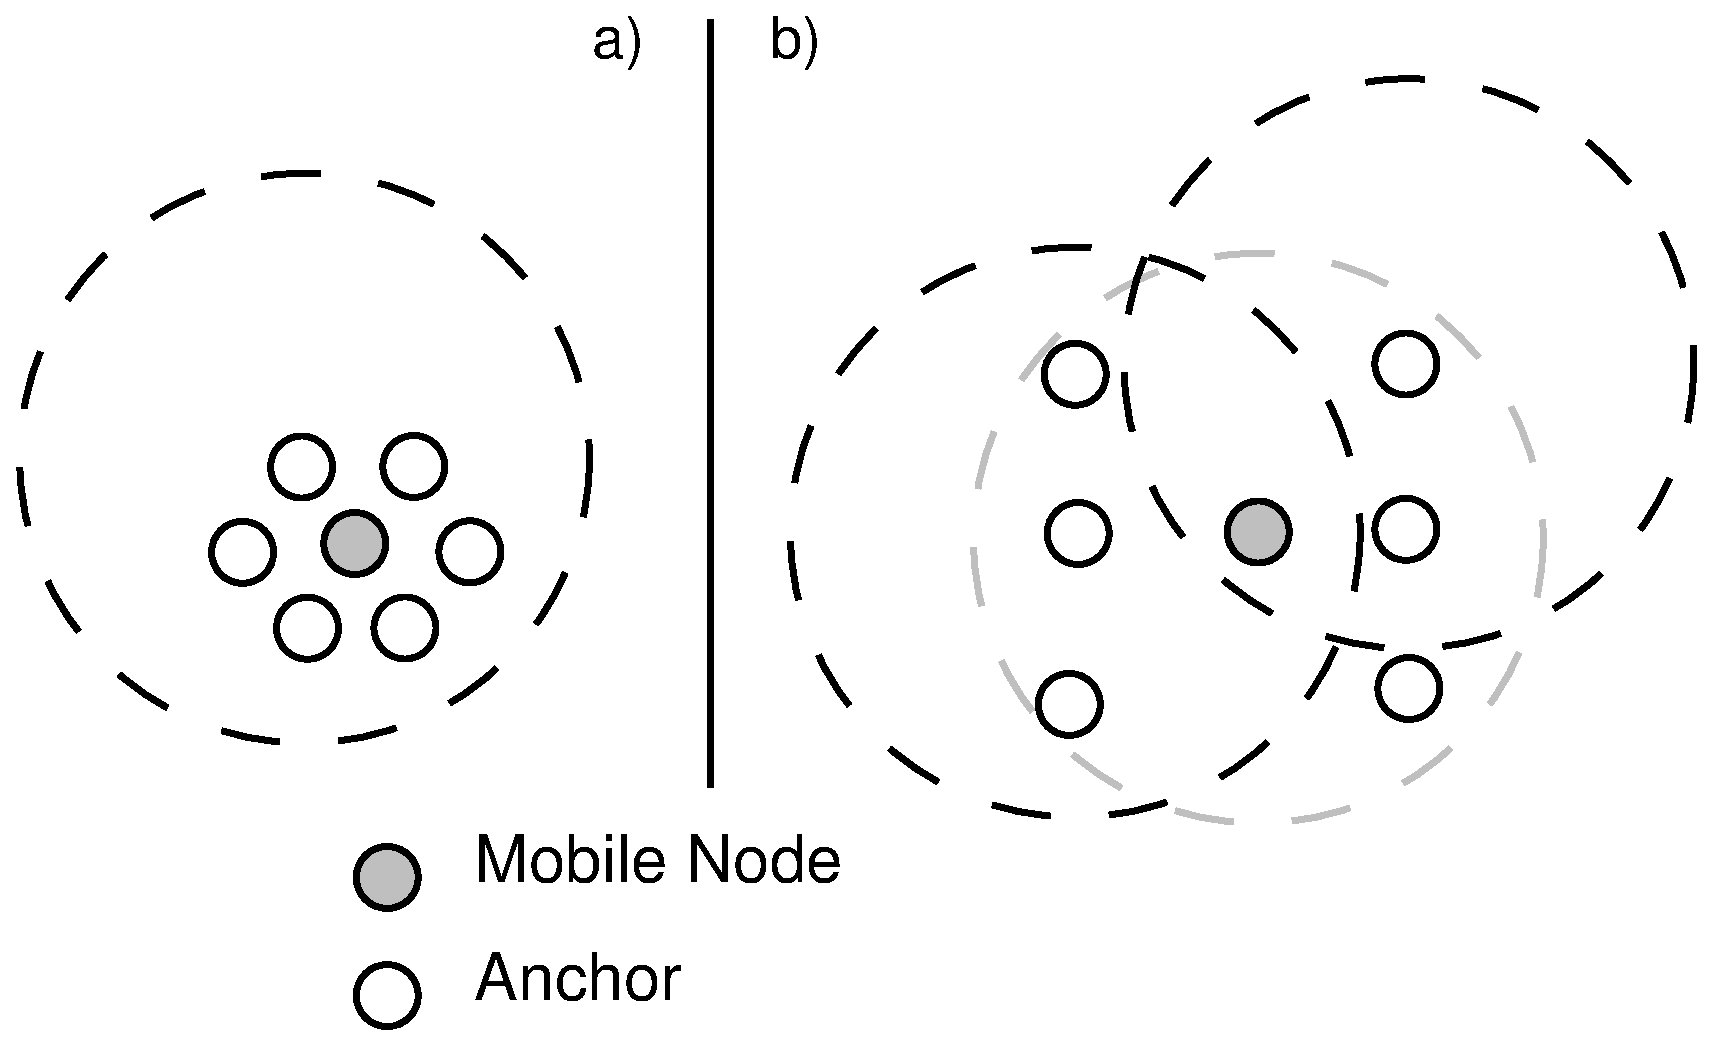
\includegraphics[width=0.5\textwidth]{hiddenvsnohidden.eps}
 \end{center}
 \caption{Scenarios avoiding (a) and forcing (b) Hidden Terminal Problem}
 \label{fig:hiddenvsnohidden}
\end{figure}

All errors caused by noise and random errors due to the channel, were disabled during this simulation. This is so, to have only errors due to 
simultaneous \acp{CCA} problem and due to Hidden Terminal Problem. Under these conditions can be assured that, if a packet is received 
incorrectly in the \ac{MN}, the reason would be one of these two problems.

As it was commented in Chapter \ref{chap:protocoldesign}: \nameref{chap:protocoldesign}, in order to avoid an unknown random time during active 
synchronization, \ac{CSMA/CA} must be disabled. If this is done, all \acp{AN} will transmit at the same time generating lots of collisions. 
To solve this situation, a random time is added by Application Layer before the packet is transmitted. This random time, will get a value
between 0 and a maximum number. In this sub-section, this maximum number goes from 1 to 30 originating 30 different simulations. This value will 
be the X axis in almost all figures. 

In order to reduce the error introduced by random numbers, each simulation will be done 1000 times.

\begin{figure}[ht]
 \begin{center}
  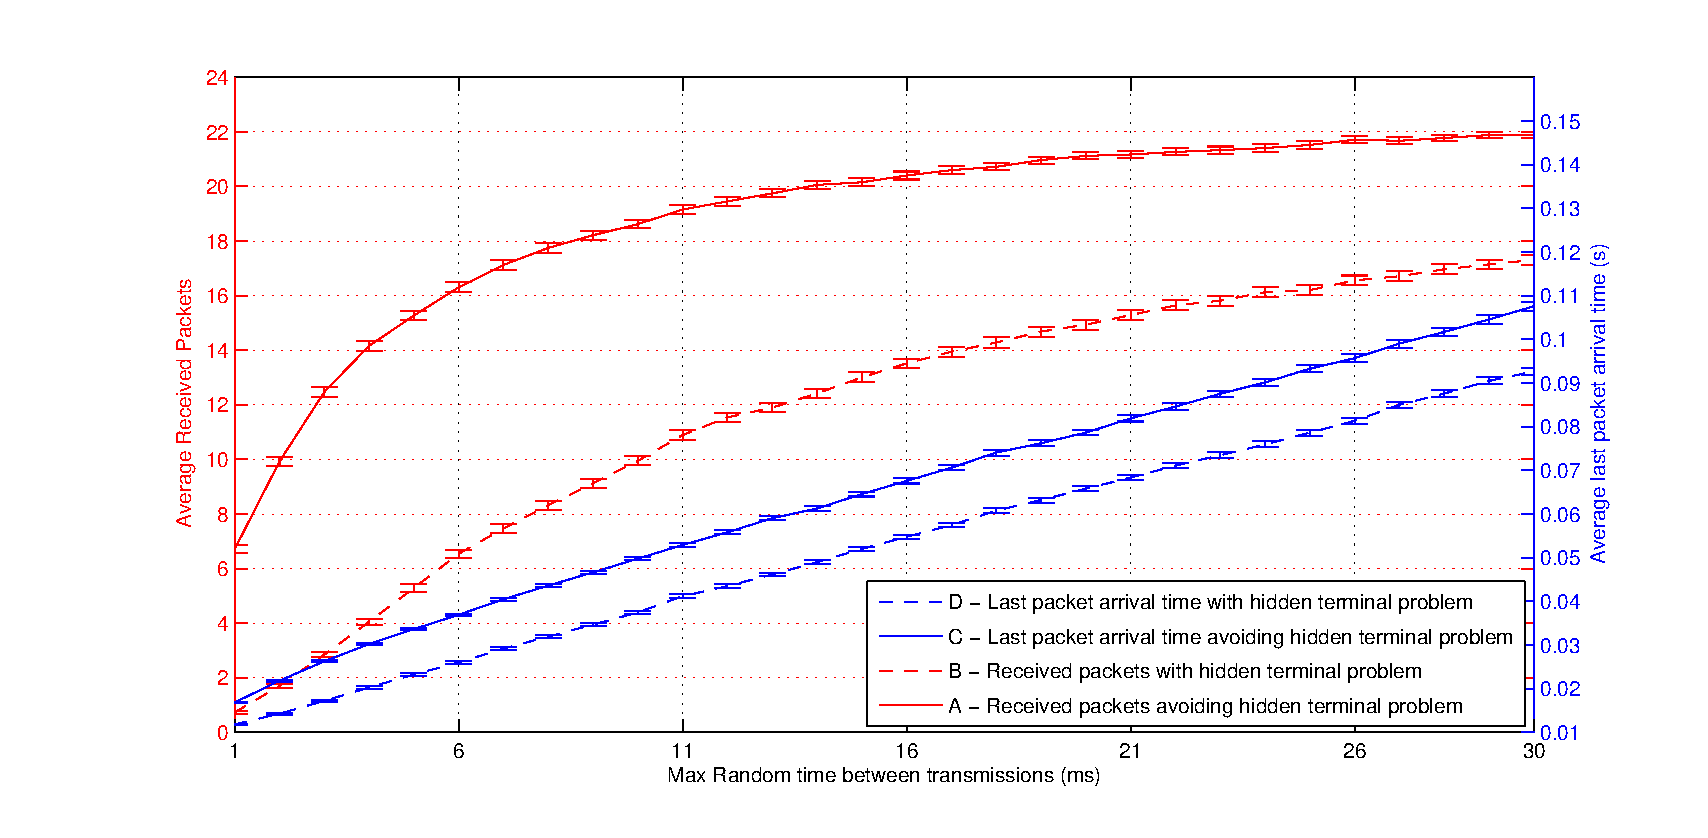
\includegraphics[width=1\textwidth]{receivedPacketsAndLastPacketArrival.eps}
 \end{center}
 \caption{Received packets in \ac{MN} and last packet arrival time}
 \label{fig:receivedPacketsAndLastPacketArrival}
\end{figure}


First simulation, gives as result \textbf{Figure \ref{fig:receivedPacketsAndLastPacketArrival}}. Here can be seen the total number of received 
packets in the \ac{MN} and the time when the last packet arrived in function of the maximum inter packet transmission time.

Both received packets lines (A and B) have a rising trajectory and both tend to 24 in the infinite. These 24 packets are the total number of 
packets sent to the network, sending to each \ac{AN} four. It can be seen that, as in the case without Hidden Terminal Problem (A) the number 
of collisions is smaller, the number of received packets in the \ac{MN} is much bigger than for the Hidden Terminal Problem case.

This Figure shows also the average arrival time of the last arrived packet in the \ac{MN}. This is not the 24$^{th}$ sent packet, as this could 
possibly collide with another. As the number of arrived packets in the case of avoiding Hidden Terminal Problem is bigger, the last packet takes more time 
to arrive to the \ac{MN}. This can be seen in the Figure as C line values are always bigger than D line ones.

\begin{figure}[ht]
 \begin{center}
  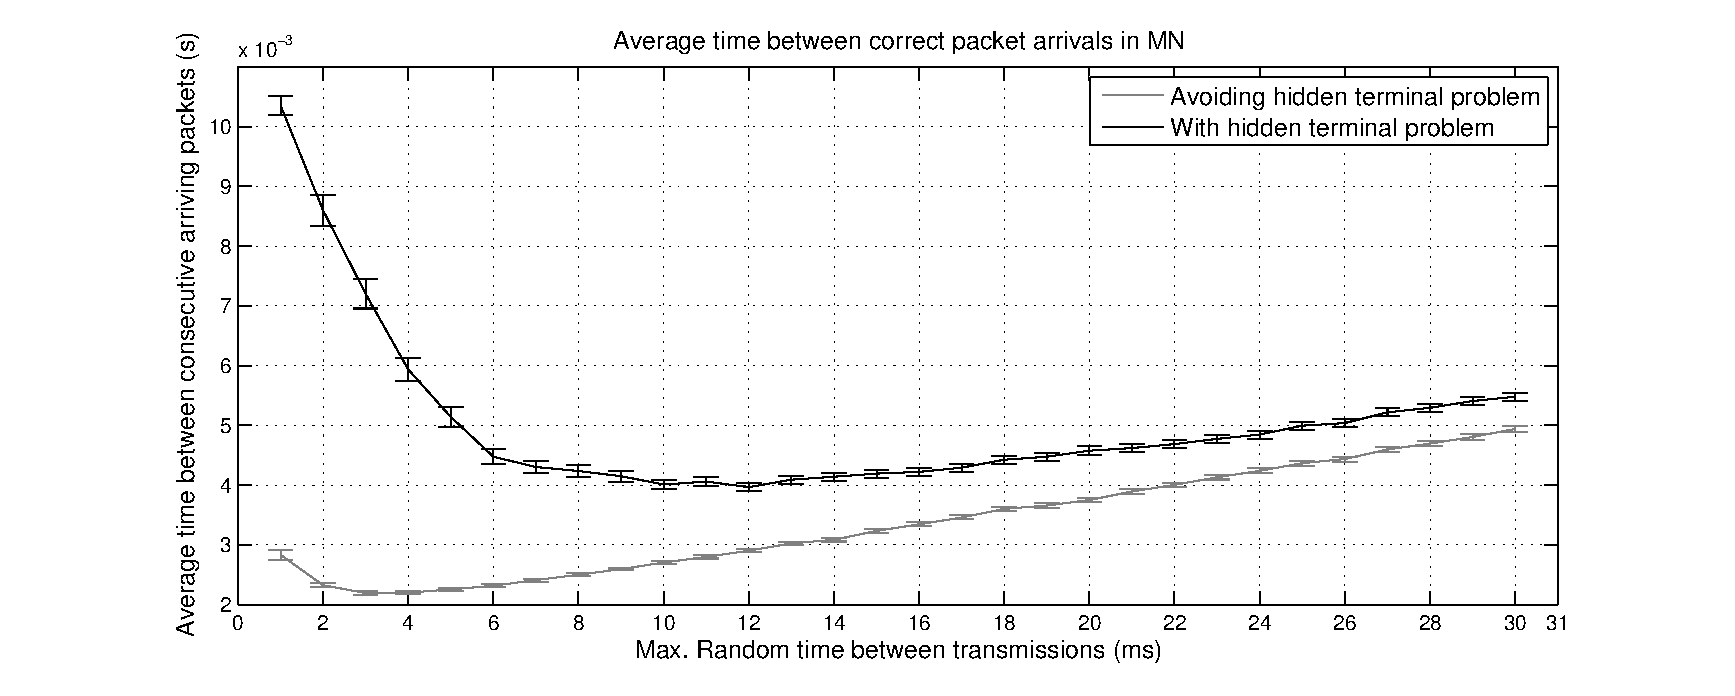
\includegraphics[width=1\textwidth]{averageTimeBetweenArrivals.eps}
 \end{center}
 \caption{Average time between arrivals in the \ac{MN}}
 \label{fig:averageTimeBetweenArrivals}
\end{figure}

\textbf{Figure \ref{fig:averageTimeBetweenArrivals}} shows the average times between packet arrivals in function of the maximum inter packet 
transmission time. This time does not represent the arrival time between two packets from the same \ac{AN}, but from any \ac{AN}. It is seen 
how for the case with Hidden Terminal Problem, the time between consecutive arrived packets is much bigger than for the case without Hidden 
Terminal Problem. Consequently the number of collisions is also bigger, needing the \ac{MN} to wait more time until it gets another valid packet.

It is logic to think, that the bigger the time between transmissions, the bigger the time between arrived packets. But, why in both cases, with 
or without Hidden Terminal Problem, for low values in X axis, the Y values start high and decrease until a certain moment where they start to 
grow again? This is because at the beginning, when the time between transmissions is low, the number of collisions is high as all \acp{AN} are 
trying to send their packets almost at the same time. As the X value becomes bigger, the number of collisions gets reduced and therefore the inter 
packet arrival time. But from the moment where the curves make their minimum, the influence of the time between transmissions becomes 
important, and makes the curve's trajectory rise again.

\begin{figure}[ht]
 \begin{center}
  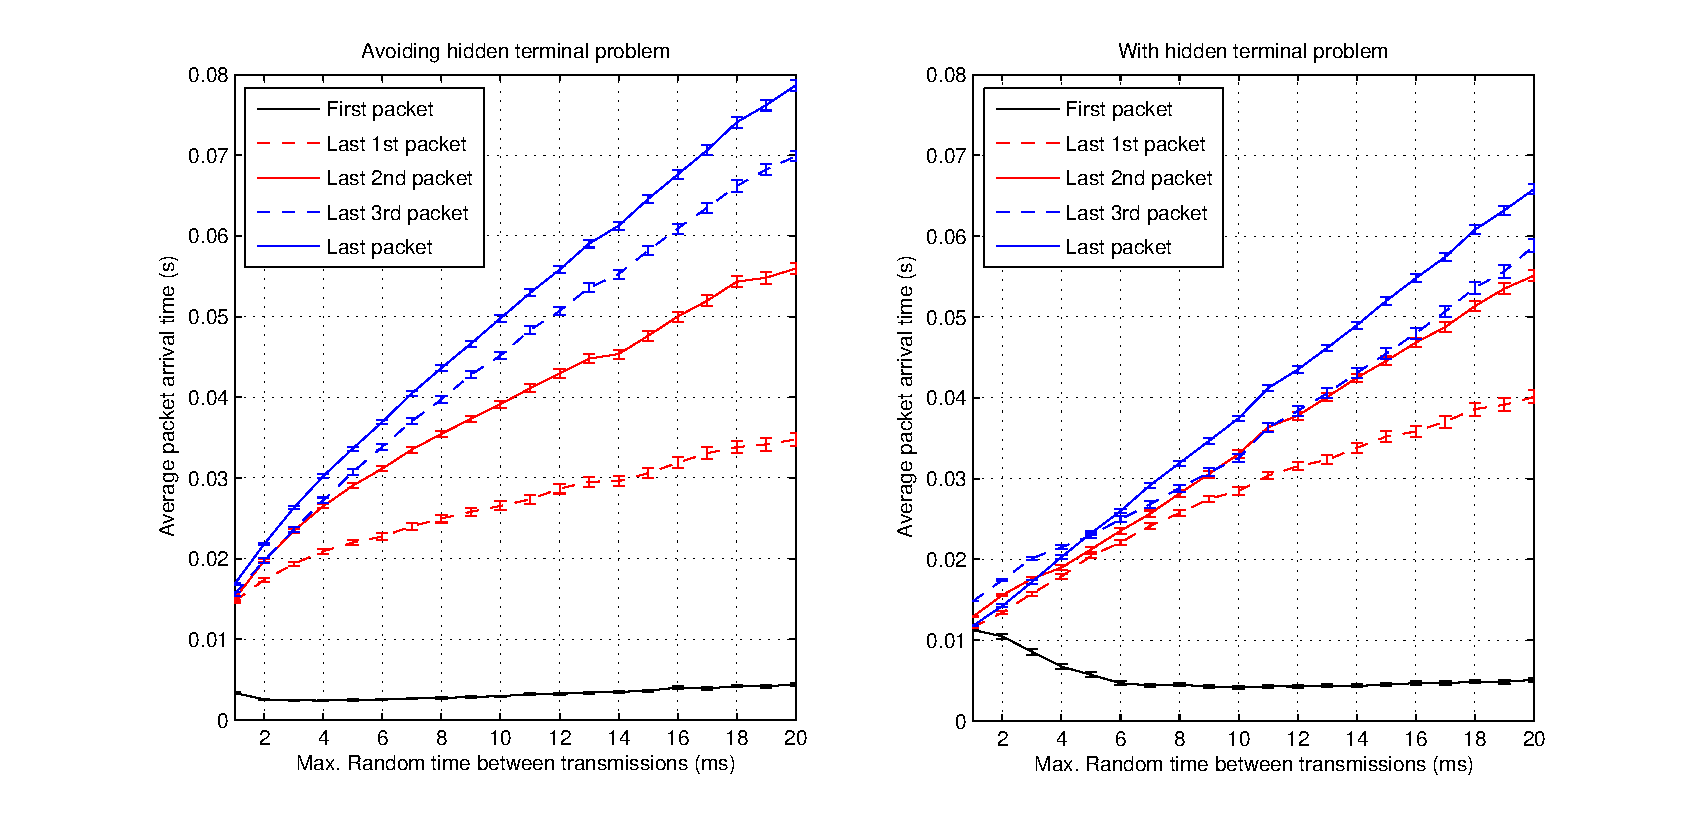
\includegraphics[width=1\textwidth]{averageDifferentTimes.eps}
 \end{center}
 \caption{Packet arrival average times}
 \label{fig:averageDifferentTimes}
\end{figure}

\textbf{Figure \ref{fig:averageDifferentTimes}} shows the average arrival time in the \ac{MN} of the first packet, the last first packet, the last
second packet, the last third packet and the last packet coming from any of the \acp{AN}.

It is comprehensible that arrival time of the first packet should be smaller than the arrival time of the last first packet, this should be smaller than
 the arrival time of the last second packet, this should be smaller than last third and this smaller than the last. But if the case with Hidden 
Terminal Problem is observed, it can be found that when time between transmissions is small, last second and last third received packets arrive later 
than last received packet. How is this possible? This happens because, due to the big number of collisions, many times only first packets arrive or many of 
them arrive after the last second or third packets. When conditions are better (higher time between transmitted packets or no Hidden Terminal Problem) 
this does not happen because many more second or third packets are delivered and therefore they will be the last packets.

It is also interesting how, unlike the right figure, for the case without Hidden Terminal Problem, the arrival time of the first packet and the arrival 
time of the last first packet are quite separated. The reason for that is that the number of collisions in this case is much smaller, and as it was seen 
in Figure \ref{fig:receivedPacketsAndLastPacketArrival}, the \ac{MN} receives much more first packets from the \acp{AN}.

As comparison of the two cases, it can be seen that for the scenario without Hidden Terminal Problem, all last packets arrive later than for the
one with Hidden Terminal Problem. This is because the \ac{MN} receives in this case much more packets due to a lower number of collisions, 
making the last packets arrive later. This lower number of collisions reduces also the arrival time of the first packet.

\begin{figure}[ht]
 \begin{center}
  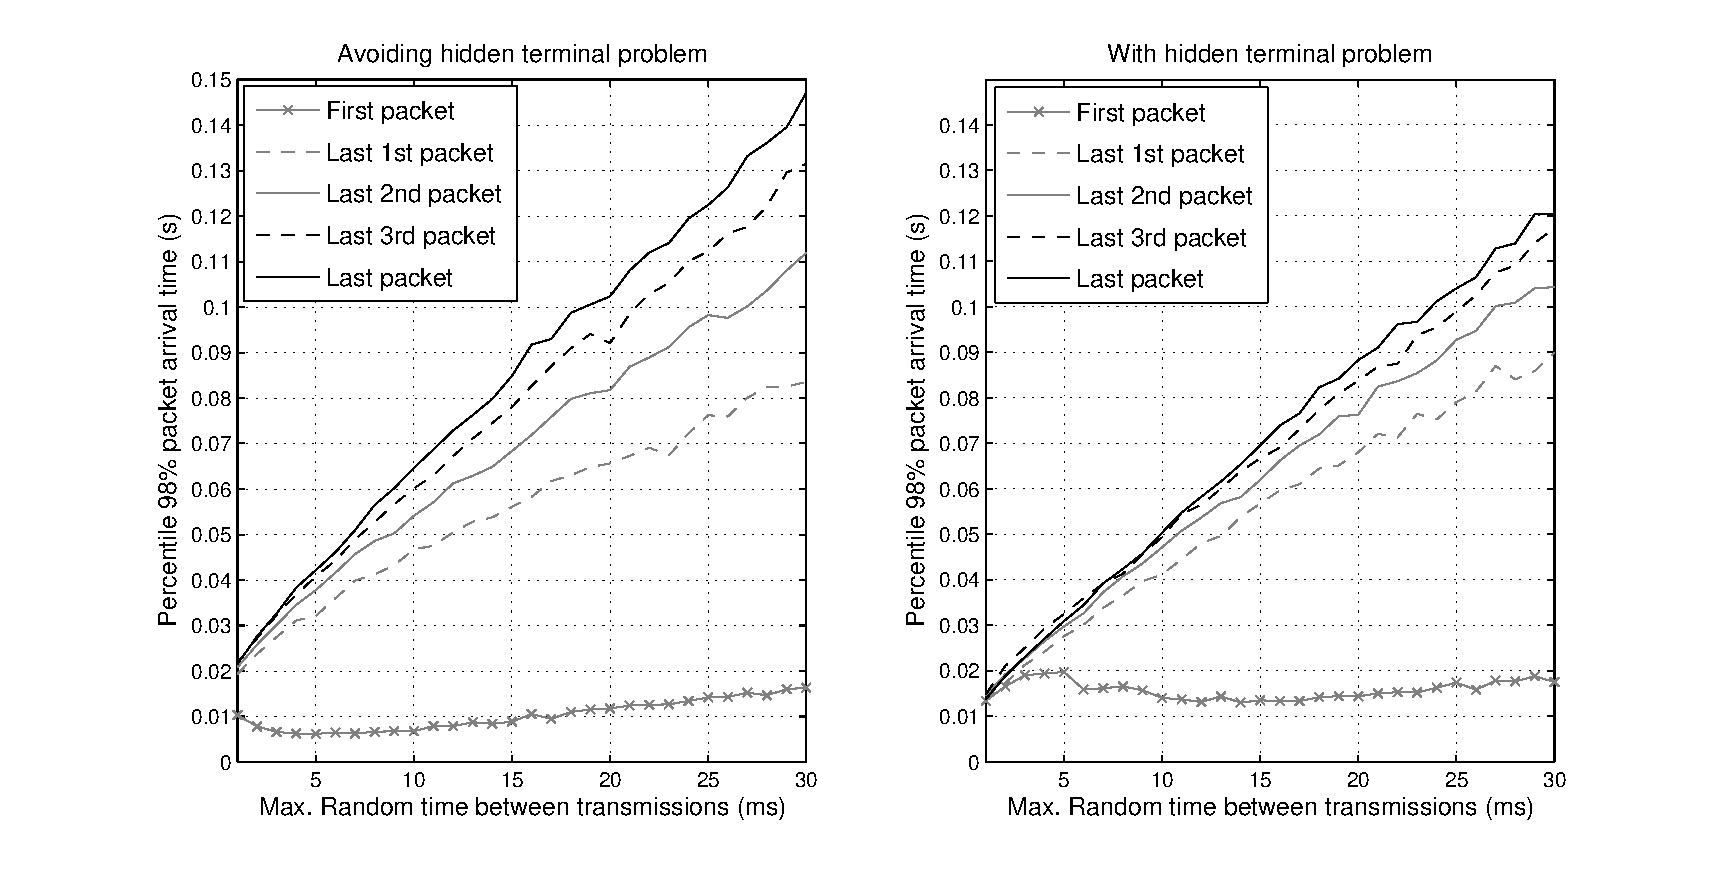
\includegraphics[width=1\textwidth]{percentil98differentTimes.eps}
 \end{center}
 \caption{$98^{th}$ Percentile of packet arrival times}
 \label{fig:percentil98differentTimes}
\end{figure}

\textbf{Figure \ref{fig:percentil98differentTimes}} does not represent an average but a $98^{th}$ percentile of the previous times. This means that 
if these times are taken as reference, in 98\% of the situations, the times are going to stay bellow these values. This is therefore a good way to get 
an acceptable top limit.

The analysis from this graphic is the same as the previous one with the only peculiarity that all times in Y axis are bigger. This is so because
this graphic represents the worst cases, not the average. For the same reason, in the case with Hidden Terminal Problem when the times between
transmissions are small, the first arrived packet time is bigger and behaves different than in Figure \ref{fig:averageDifferentTimes}.

\subsection{Slotted vs. Random Transmission}

The aim of this sub-section is to compare the random and the slotted transmission during the Sync Phase of the protocol. As slotted case seems to be
much better than random case, the step to make is looking for the best case in random transmission. To find this best case an optimum number
of broadcasted packets and time between transmissions should be found.

The scenario has 80 \acp{MN} uniformly and randomly distributed along the playground, and 30, 40, 50, 60 and 70 \acp{AN} distributed the same way.
There is therefore Hidden Terminal Problem.

In order to reduce the error introduced by random numbers, each simulation is done 100 times. Data will be measured in the \acp{MN}, which
are dispersed all over the playground. This will influence their values depending on the load of every network part. That is why first 
an average of the 80 nodes will be done to get the average situation of a node, and this will be followed by the average of the 100 repetitions.

\subsubsection{Checking the best inter packet random time}

In this scenario, each \ac{AN} sends as many packets as it can during the Sync Phase time defined by the slots. First, Computer calculates the number of
slots and multiplies it by \textit{syncPacketsPerSyncPhase} (in this case 3) to obtain the Sync Phase time. This simulation will be done for different
numbers of \acp{AN} and different maximum random times between transmissions from 1 to 30 ms. After repeating each case 100 times,
\textbf{Figure \ref{fig:randomTimeCheckingTheBestInterpacketRandomTime}} is obtained.

\begin{figure}[ht]
 \begin{center}
  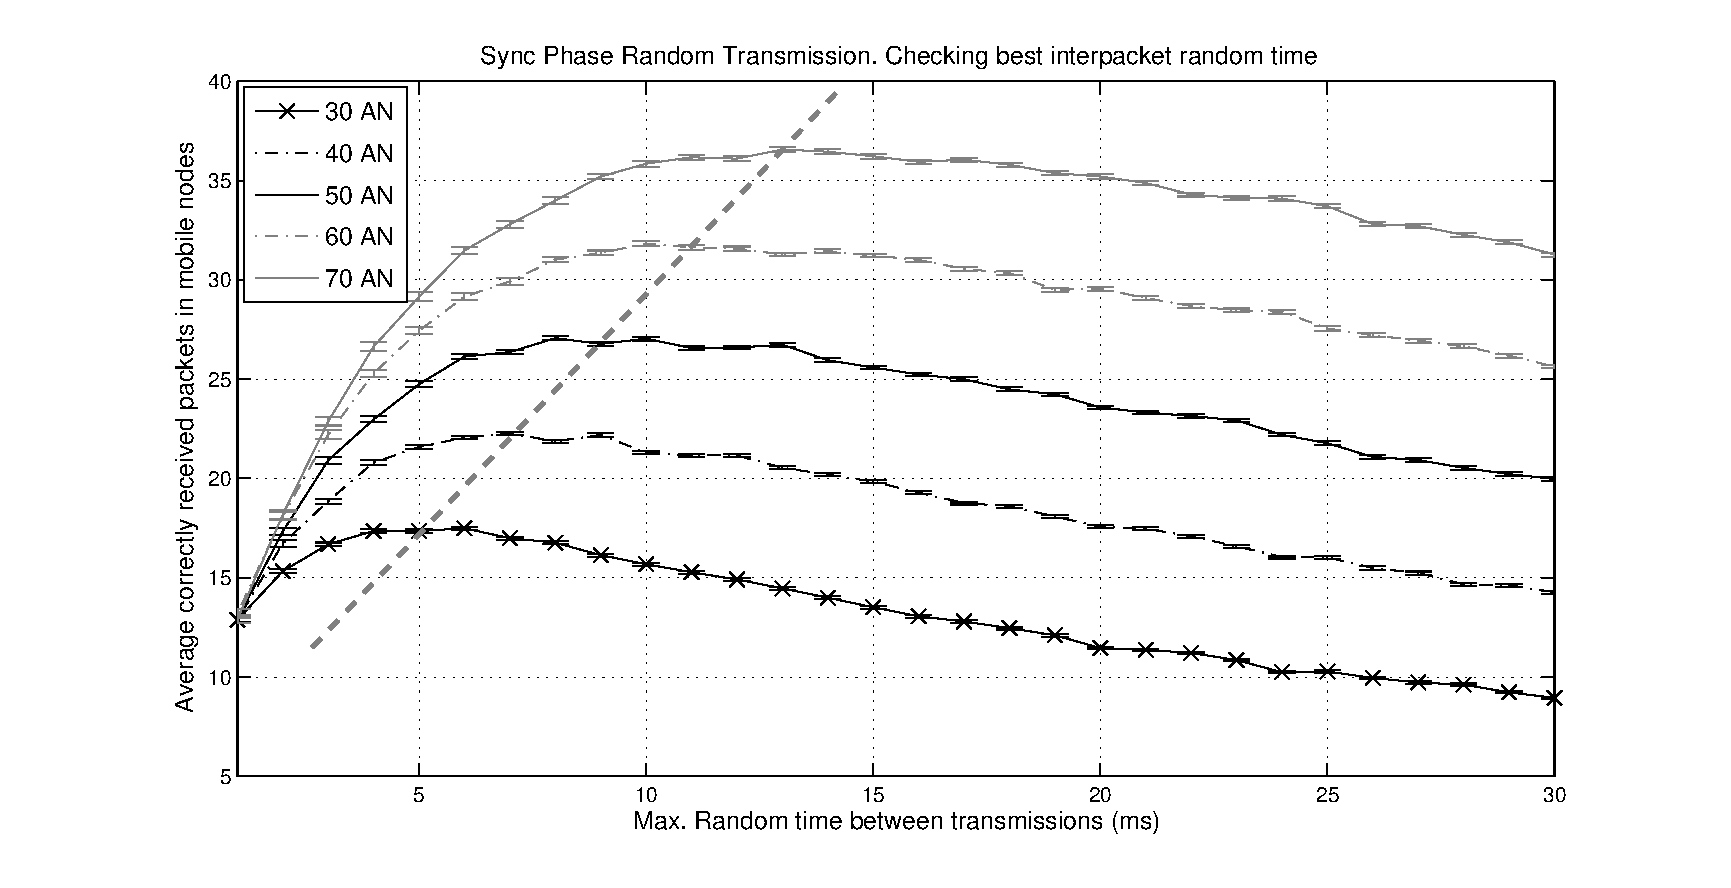
\includegraphics[width=1\textwidth]{randomTimeCheckingTheBestInterpacketRandomTime.eps}
 \end{center}
 \caption{Checking the best time between random transmissions}
 \label{fig:randomTimeCheckingTheBestInterpacketRandomTime}
\end{figure}

In this figure is shown that if the time between transmissions is small, the number of delivered packets is also small. This occurs due to the 
collisions. When the time between transmissions grows, the number of correctly received packets also does, until a maximum is reached and then 
the number decreases again. The reason for this is that the bigger the time between transmissions, the less the number of packets that fit 
in the fixed Sync Phase time. When in Figure \ref{fig:receivedPacketsAndLastPacketArrival} there was no time limit, it could be seen how the 
received packets number did only grow.

From Figure \ref{fig:randomTimeCheckingTheBestInterpacketRandomTime}, it can also be seen that the more \acp{AN} there are, the more received packets and
the later the maximum. This maximum comes later because as the number of \acp{AN} is bigger, there are also more collisions, being its effect in the 
number of delivered packets bigger, compared to the time between transmissions. As the number of slots is bigger and therefore the Sync Phase time, the 
time between transmissions influence will come later.

The gray discontinuous line was drawn following the maximum points for every curve. This line gives us the optimum waiting time between transmissions to 
be set for any number of \acp{AN}. Taking a smaller value generates more collisions and a bigger value makes the number of delivered packets smaller due
to the lack of time in the phase.

\subsubsection{Checking the best number of sent packets per \ac{AN}}

In this scenario, each \ac{AN} sends a maximum number of packets from 3 to 16 during the Sync Phase time defined by the slots. First, Computer calculates 
the number of slots and multiplies it by \textit{syncPacketsPerSyncPhase} (in this case 3) to obtain the Sync Phase time. This simulation will be done 
for different number of \acp{AN} where the previous optimal maximum random times between transmissions will be taken (see Table
\ref{tab:optimalTransmitTimes}). After repeating each case 100 times, \textbf{Figure \ref{fig:randomTimeCheckingTheBestNumberOfSentPacketsForAnchor}} 
is obtained.

\begin{table}
 \begin{center}
  \begin{tabular}{|l|c|}
   %\noalign{\vspace*{0.5cm}}
   \hline
   30 \acp{AN} & 5 ms \\
   \hline
   40 \acp{AN} & 7 ms \\
   \hline
   50 \acp{AN} & 9 ms \\
   \hline
   60 \acp{AN} & 11 ms \\
   \hline
   70 \acp{AN} & 13 ms \\
   \hline
  \end{tabular}
  \caption{Optimal maximal random times between \ac{AN} transmissions}
  \label{tab:optimalTransmitTimes}
 \end{center}
\end{table}

\begin{figure}[ht]
 \begin{center}
  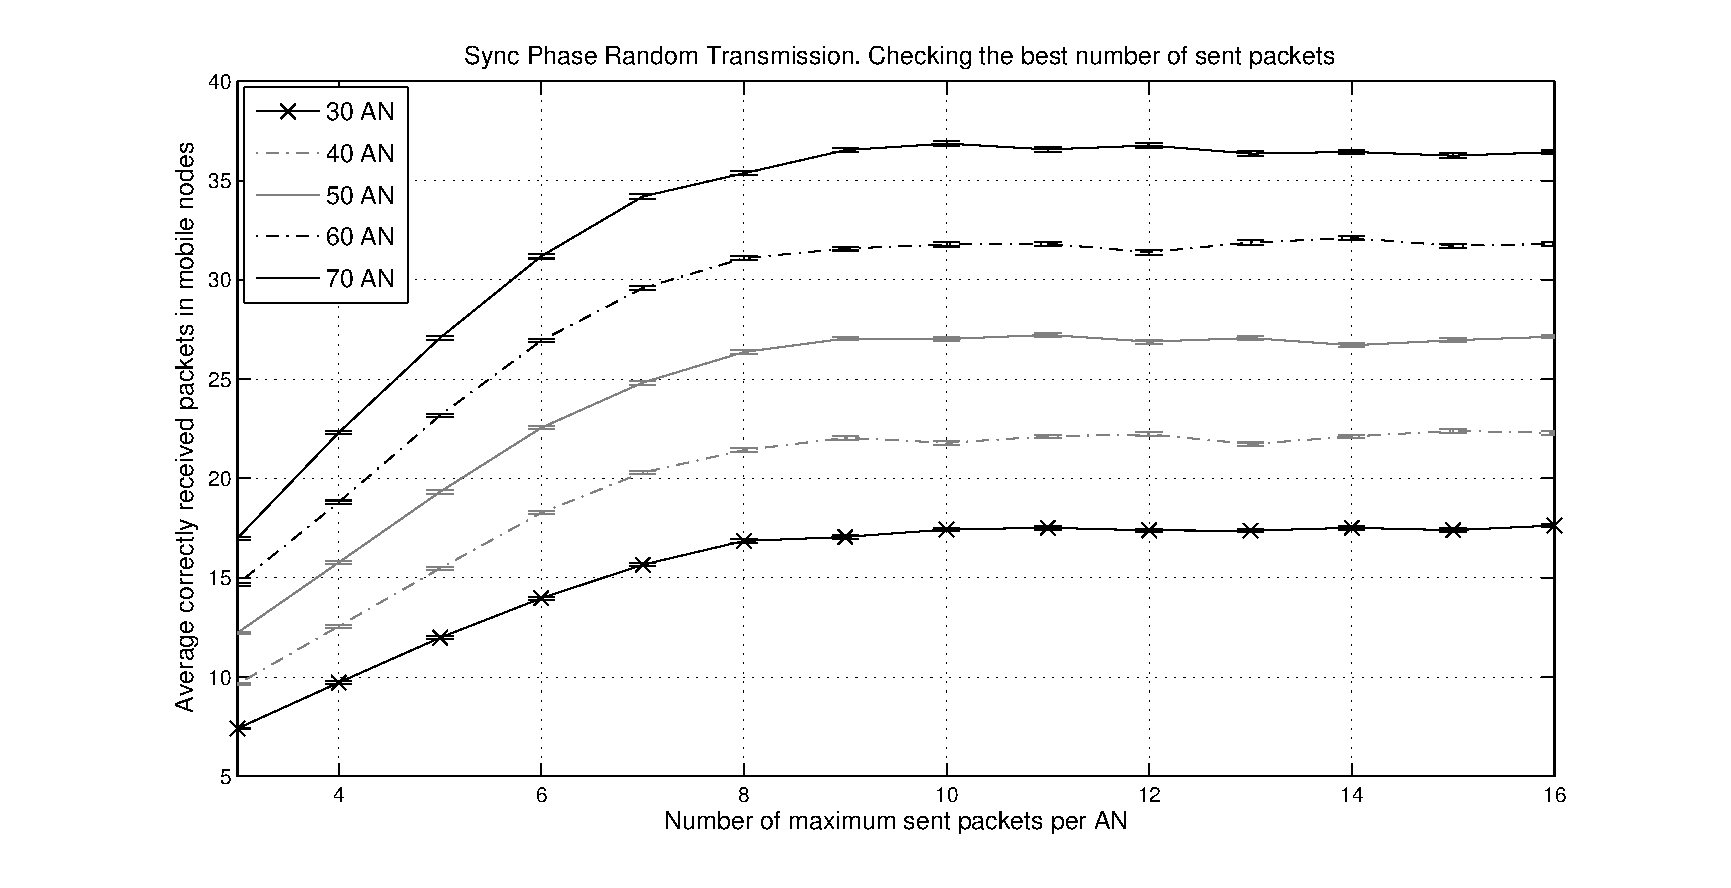
\includegraphics[width=1\textwidth]{randomTimeCheckingTheBestNumberOfSentPacketsForAnchor.eps}
 \end{center}
 \caption{Checking the best number of sent packets per \ac{AN}}
 \label{fig:randomTimeCheckingTheBestNumberOfSentPacketsForAnchor}
\end{figure}

It can be clearly seen in the figure, how the average number of received packets in the \acp{MN} increases until it reaches a maximum (approximately
with 10 sent packets). This is can be explained with the fixed Sync Phase time, where is no time for more packets to arrive. Therefore, ten is defined 
as the maximum number of packets to be sent by an \ac{AN}. The reason for this limit is that when an \ac{AN} has already reached this maximum sent packets 
number per Sync Phase, it will stop sending more, leaving the channel free for the rest of the \acp{AN} to transmit.

\subsubsection{Slotted vs. Best Random case comparison}

Both alternatives will be compared in a first approach checking the average number of packets received by the \acp{MN} in different situations. In 
all situations, cases with 30, 40, 50, 60 and 70 \acp{AN} will be studied. In the comparison will be included the following situations: 
slotted case, best random transmissions case, worst random transmissions case ($T=1 ms$) and two random transmissions cases between worst and best cases
($T=3ms$ and $T=5ms$), in which T is the maximum random time between transmissions. In all cases the number of transmitted packets per \ac{AN} will be 10.

\begin{figure}[ht]
 \begin{center}
  \includegraphics[width=1\textwidth]{slottedVsRandomAverageReceivedPackets.eps}
 \end{center}
 \caption{Slotted vs. Random cases comparison for number of received packets in \ac{MN}}
 \label{fig:slottedVsRandomAverageReceivedPackets}
\end{figure}

\textbf{Figure \ref{fig:slottedVsRandomAverageReceivedPackets}} shows how in all situations, in the slotted case \acp{MN} received more packets then in
any of the random cases. It can also be seen that this difference gets bigger when the number of \acp{AN} arises.

As a second comparison between the best case for random transmissions and the slotted case, the number of first, second, third, fourth, \ldots, eighth
packets from an \ac{AN} received in the \ac{MN}, will be studied. Results can be seen in \textbf{Figure \ref{fig:numberOf1st2ndPacketsReceived}}.

\begin{figure}[ht]
 \begin{center}
  \includegraphics[width=1\textwidth]{numberOf1st2ndPacketsReceived.eps}
 \end{center}
 \caption{Number of $1^{st}$, $2^{nd}$, $3^{rd}$ \ldots, $8^{th}$ received packets in \acp{MN} from an \ac{AN}}
 \label{fig:numberOf1st2ndPacketsReceived}
\end{figure}

In both graphics can be appreciated that the more \acp{AN} there are, the more received packets in the \acp{MN}. It can be seen as well, that
for the slotted case, the number of received packets is bigger than for the random case (as it was already proved).

In the graphic on the left, it is shown how the number of first packets received is bigger than the number of second packets. How the number of 
second packets received is bigger than the number of third packets, etc. It can also be seen how this reduction occurs in a gradual way unlike 
in the graphic on the right, where a stair-shaped behavior can be appreciated.

As \textit{syncPacketsPerSyncPhase} = 3, the Sync Phase will be divided into 3 identical sub phases. This means that all packets sent in one sub 
phase, will be sent in the other two. That is why the number of first, second and third packets is the same, as well as the number of fourth, fifth 
and sixth, and the number of seventh and eighth.

In the graphic, slot reuse can also be appreciated. Anytime a packet is sent more than 3 times (\textit{syncPacketsPerSyncPhase}), is due to slot reusing. 
That justifies why for example for the 30 \acp{AN} case, no seventh or eighth packets where sent, reuse here was not so big.

As a last comparison between slotted case and best random case, Packet arrival times in the \acp{MN} will be studied, getting \textbf{Figure
\ref{fig:Lastarrivalpackettimes}}. For a good understanding of this figure, X axis should be clarified. X axis has numbers
going from 1 to 11. Number from 1 to 8 represent the $1^{st}$, $2^{nd}$, $3^{rd}$ \ldots, $8^{th}$ last received packet in the \acp{MN}. Number 9 
represents the first packet arrived in the \acp{MN}. Number 10 represents the last packet arrived in the \acp{MN}. And number 11 represents the elapsed 
time between arrived packets in the \acp{MN}.

\begin{figure}[ht]
 \begin{center}
  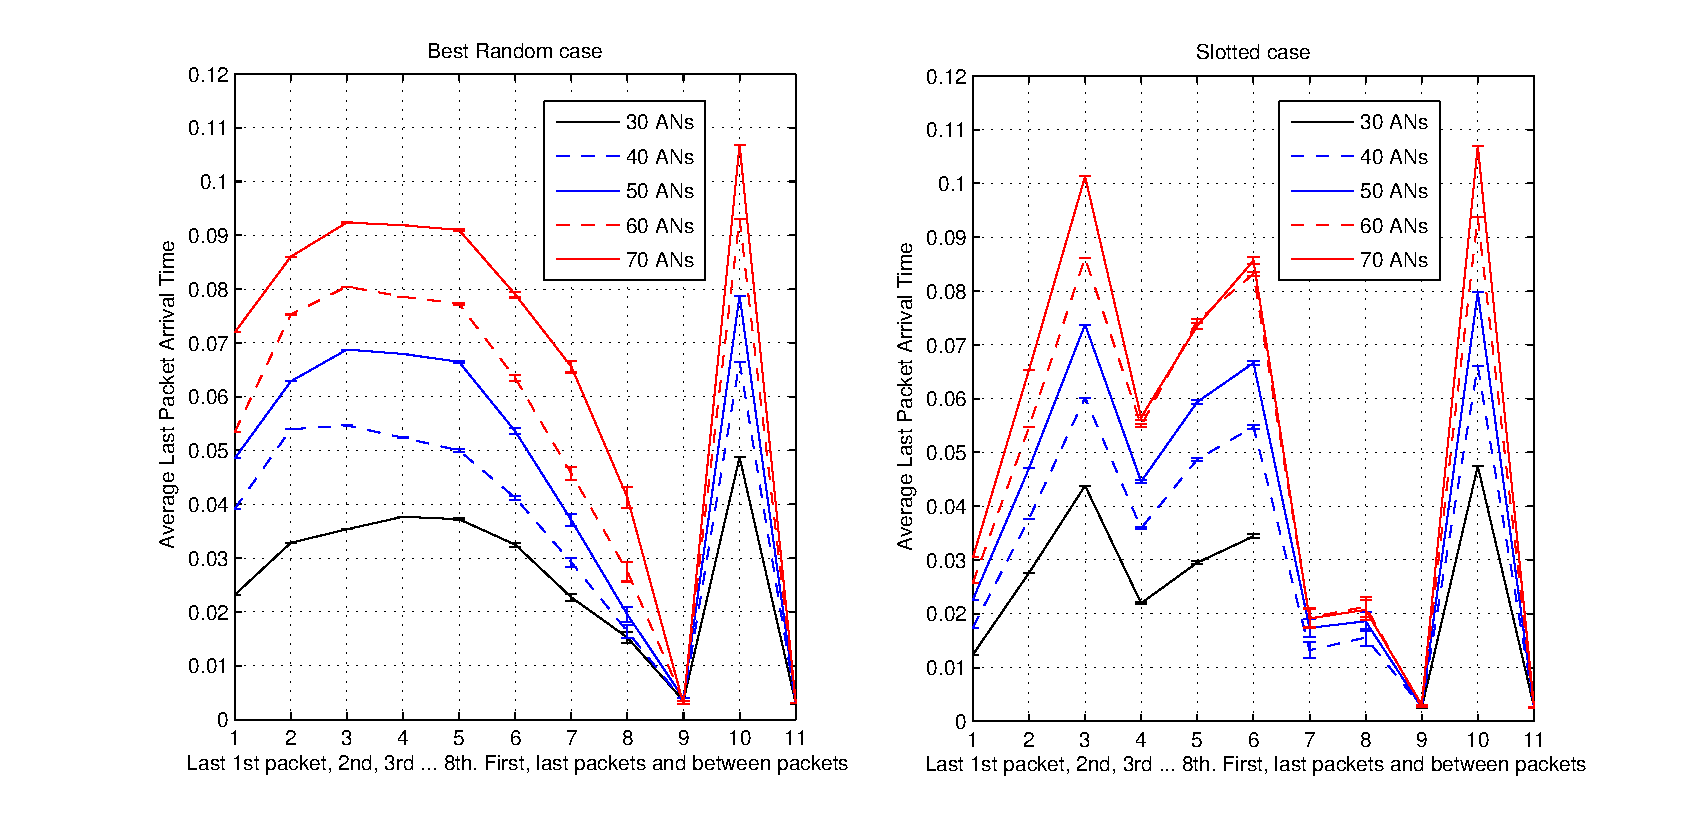
\includegraphics[width=1\textwidth]{Lastarrivalpackettimes.eps}
 \end{center}
 \caption{Different packet arrival times in the \acp{MN}}
 \label{fig:Lastarrivalpackettimes}
\end{figure}

Like for the case in Figure \ref{fig:numberOf1st2ndPacketsReceived}, the more the \acp{AN} in the network, the bigger the time the \acp{MN} have to wait 
until they get the last packet.

Comparing both, right and left graphics, it can be seen that the arrival times for the first packet ($X=9$), the last packet ($X=10$) and the inter arrival 
time ($X=11$), are very similar. This is because it depends mainly on the duration of the Sync Phase more than on the way the packets are sent. 
Looking at the arrival time of the last packet ($X=10$), the length of the Sync Phase can be deduced.

When looking to X axis values from 1 to 8, many differences can be observed.

In the case of the graphic on the left (best random case), it can be seen that for small last $X^{th}$ received packet, the times grow with X. 
This is because all \acp{MN} receive many $1^{st}$, $2^{nd}$ or $3^{rd}$ packets, and the last of the $1^{st}$ packets should arrive 
before the last of the $2^{nd}$ and so on. But, why is it not like this until the last packet? The reason is that not many \acp{AN} are able to send
$5^{th}$, $6^{th}$, $7^{th}$ or $8^{th}$ packets. This way, as the $3^{rd}$ or $4^{th}$ packets are the maximum packets \acp{AN} can send, 
these packets will be delivered at the end of the Sync Phase, raising therefore the average arrival time for this kind of packets.

In the slotted case graphic (on the right), the idea is the same as expressed before. The only difference is that, like in Figure 
\ref{fig:numberOf1st2ndPacketsReceived}, as \textit{syncPacketsPerSyncPhase} = 3, all behaviors are grouped, and it can be seen that $1^{st}$, 
$2^{nd}$ and $3^{rd}$ last packets are together in one group. $4^{th}$, $5^{th}$ and $6^{th}$ last packets are in another group, and 
$7^{th}$ and $8^{th}$ are in a further one. In each group, whenever the \ac{AN} sends the first of the packets ($1^{st}$, $4^{th}$ or $7^{th}$), the 
next two will also be sent. As Sync Phase is divided in 3 identical sub phases, which come one after another in time, the arrival time of 
each packet in each group grows with X.

Here, like in Figure \ref{fig:numberOf1st2ndPacketsReceived}, the reusability of the slots can also be observed. Seeing for example for the 
30 \acp{AN} case, that no seventh or eighth packets were sent because the reuse here was not so big.

\subsubsection{Slot Number vs. \acp{AN} Number}

This sub-section's aim is checking how good the algorithm calculates the slot distribution among the \acp{AN}. For this purpose, an scenario 
with different number of \acp{AN} will be used. In this scenario, the slots will be calculated by a Computer as described in Chapter 
\ref{chap:protocoldesign} (\nameref{chap:protocoldesign}). Like in previous simulations, this scenario will be simulated 100 times. It has to
be taken into account that Computer takes also its own slot, this can be seen like \acp{AN} number is one unit bigger.

\begin{figure}[ht]
 \begin{center}
  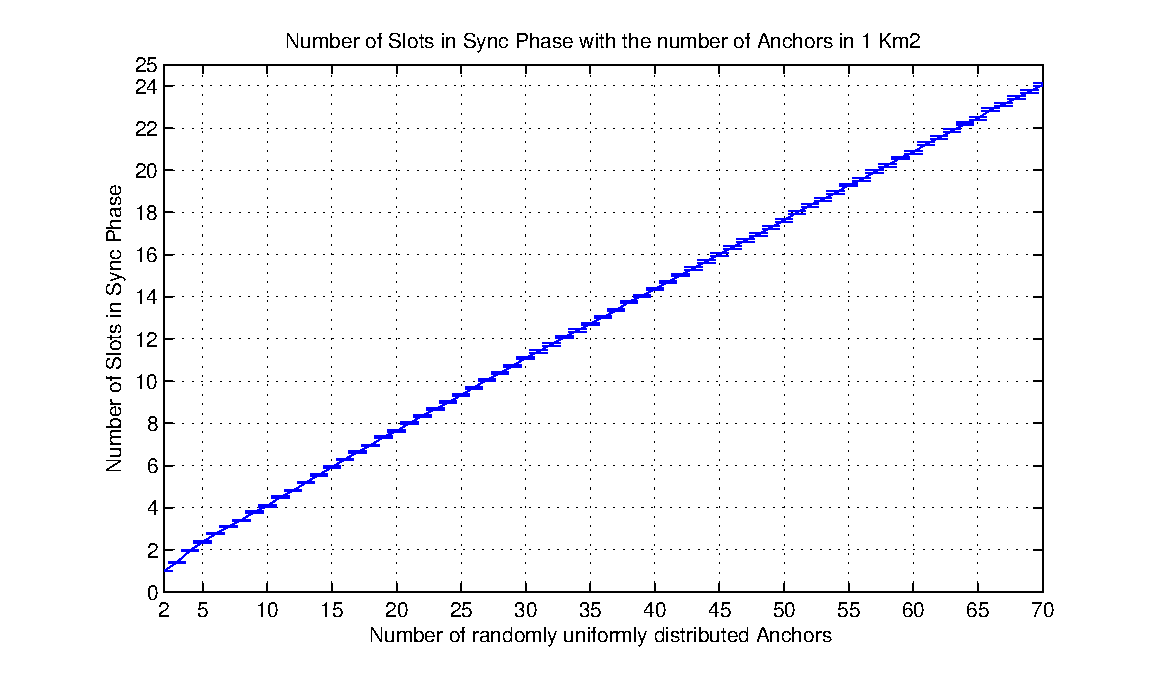
\includegraphics[width=1\textwidth]{numberOfSlotsWithTheAnchorDensity.eps}
 \end{center}
 \caption{Slot Number for a variable \acp{AN} density}
 \label{fig:numberOfSlotsWithTheAnchorDensity}
\end{figure}

\textbf{Figure \ref{fig:numberOfSlotsWithTheAnchorDensity}} is the result of simulating a 1 $Km^2$ playground with a number of \acp{AN} going from 
2 to 70, as the playground is fixed and only the number of nodes increases, it could be said that \acp{AN} density increases. When \acp{AN} density 
increases, and as \acp{AN} range stays constant, the number of neighbors for each \ac{AN} increases also. For that reason, the number of slots grows 
with the number of \acp{AN}, as it can be seen in the figure.

\begin{figure}[ht]
 \begin{center}
  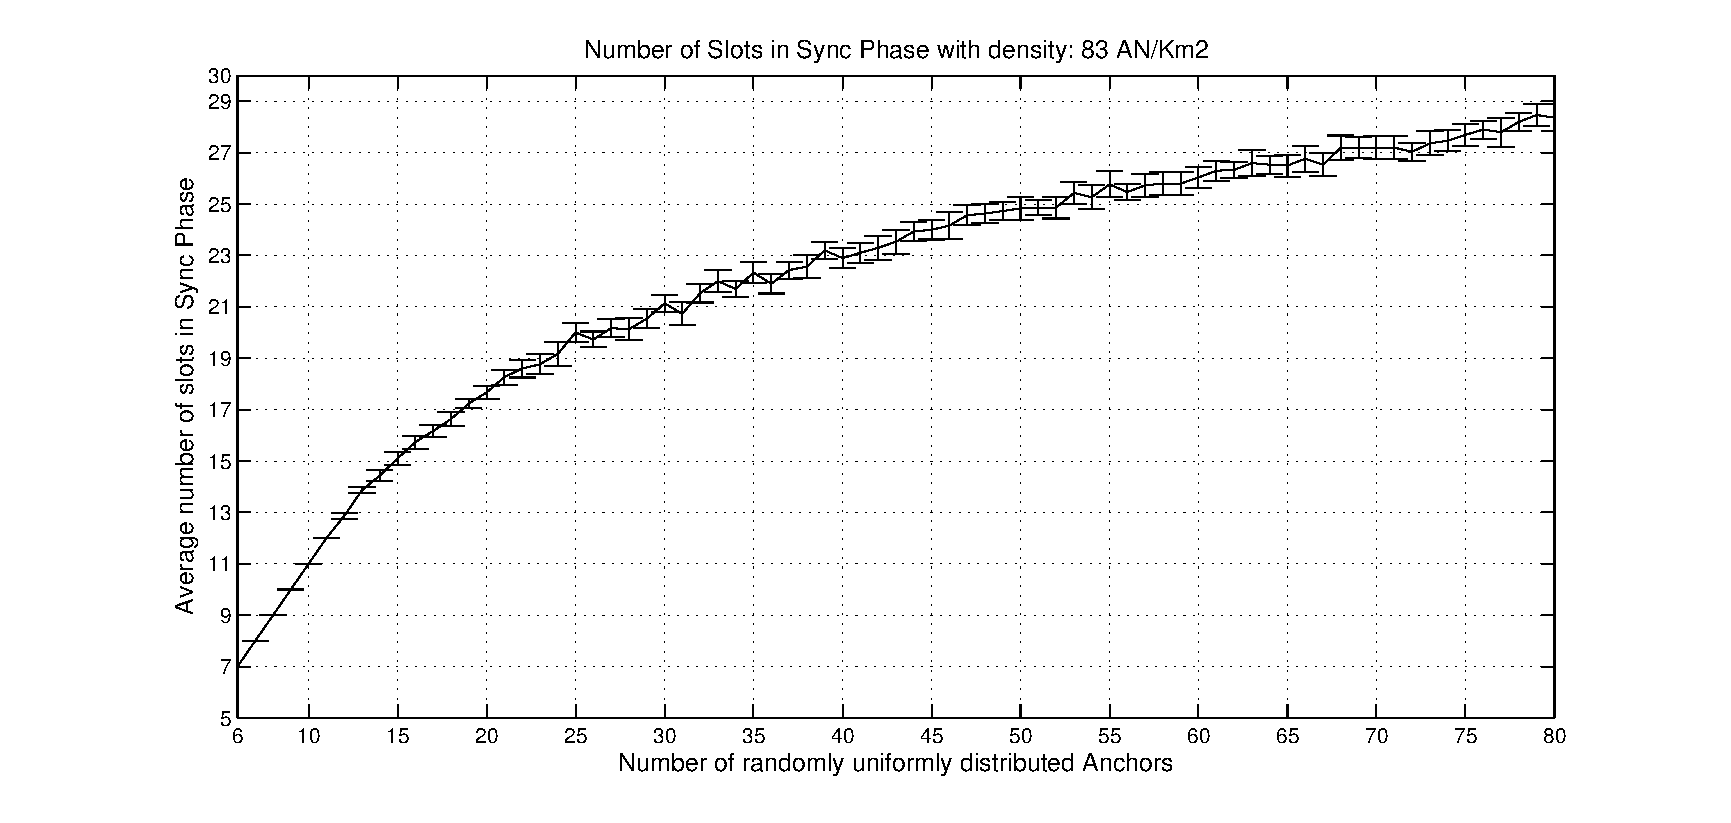
\includegraphics[width=1\textwidth]{numberOfSlotsWithTheSameDensity.eps}
 \end{center}
 \caption{Slot Number for a fixed \acp{AN} density}
 \label{fig:numberOfSlotsWithTheSameDensity}
\end{figure}

\textbf{Figure \ref{fig:numberOfSlotsWithTheSameDensity}} is obtained simulating 6 to 80 nodes with a minimum separation of 80 meters between 
them. Playground is calculated dynamically with these parameters to have always a 83 $\acp{AN}/Km^2$ density. As \acp{AN} density remains constant,
the number of neighbors an \ac{AN} has also does. This means the reusability of the slots will grow with the number of \acp{AN}. The reusability can be
observed in the figure: when the number of \acp{AN} grow, the number of slots does not grow linearly like in Figure \ref{fig:numberOfSlotsWithTheAnchorDensity}.

\paragraph{Conclusion.} From all these results can be extracted that slotted transmission is better than even the best case of random transmission. 
Slotted transmission will be therefore the one used during the Sync Phase in the complete protocol analysis.

\section{Framework simulation and analysis}

The aim of this section, is to analyze by using different configurations the performance of the network for parameters like traffic or energy 
consumption among others.

The proposed scenario for these simulations is formed by 25 \acp{AN} distributed forming a grid, 60 \acp{MN} randomly and uniformly distributed in the
playground and a Computer. An example for this scenario, with a size of 700 x 700 m, can be seen in Figure \ref{fig:finalscenario} . The \acp{AN} 
are distributed forming a grid to avoid the necessity to make a more complex routing protocol (explained in Chapter \ref{chap:protocolimplementation}: 
\nameref{chap:protocolimplementation}). Grid was also chosen because in the literature it was proven to be a good way to study a network \cite{GridNetworks}.

From the proposed grid, and with the help of the algorithm to assign slots (Sub-Section \ref{subsec:slottedsyncphase}: 
\nameref{subsec:slottedsyncphase}), it was obtained that 9 slots is the number of slots needed to avoid Hidden Terminal Problem. These slots have the 
following distribution of \acp{AN}:

\begin{verbatim}
      Slot 0: 0, 3, 15, 18
      Slot 1: 1, 4, 16, 19
      Slot 2: 2, 17
      Slot 3: 5, 8, 20, 23
      Slot 4: 6, 9, 21, 24
      Slot 5: 7, 22
      Slot 6: 10, 13
      Slot 7: 11, 14
      Slot 8: 12
\end{verbatim}

\begin{figure}[ht]
 \begin{center}
  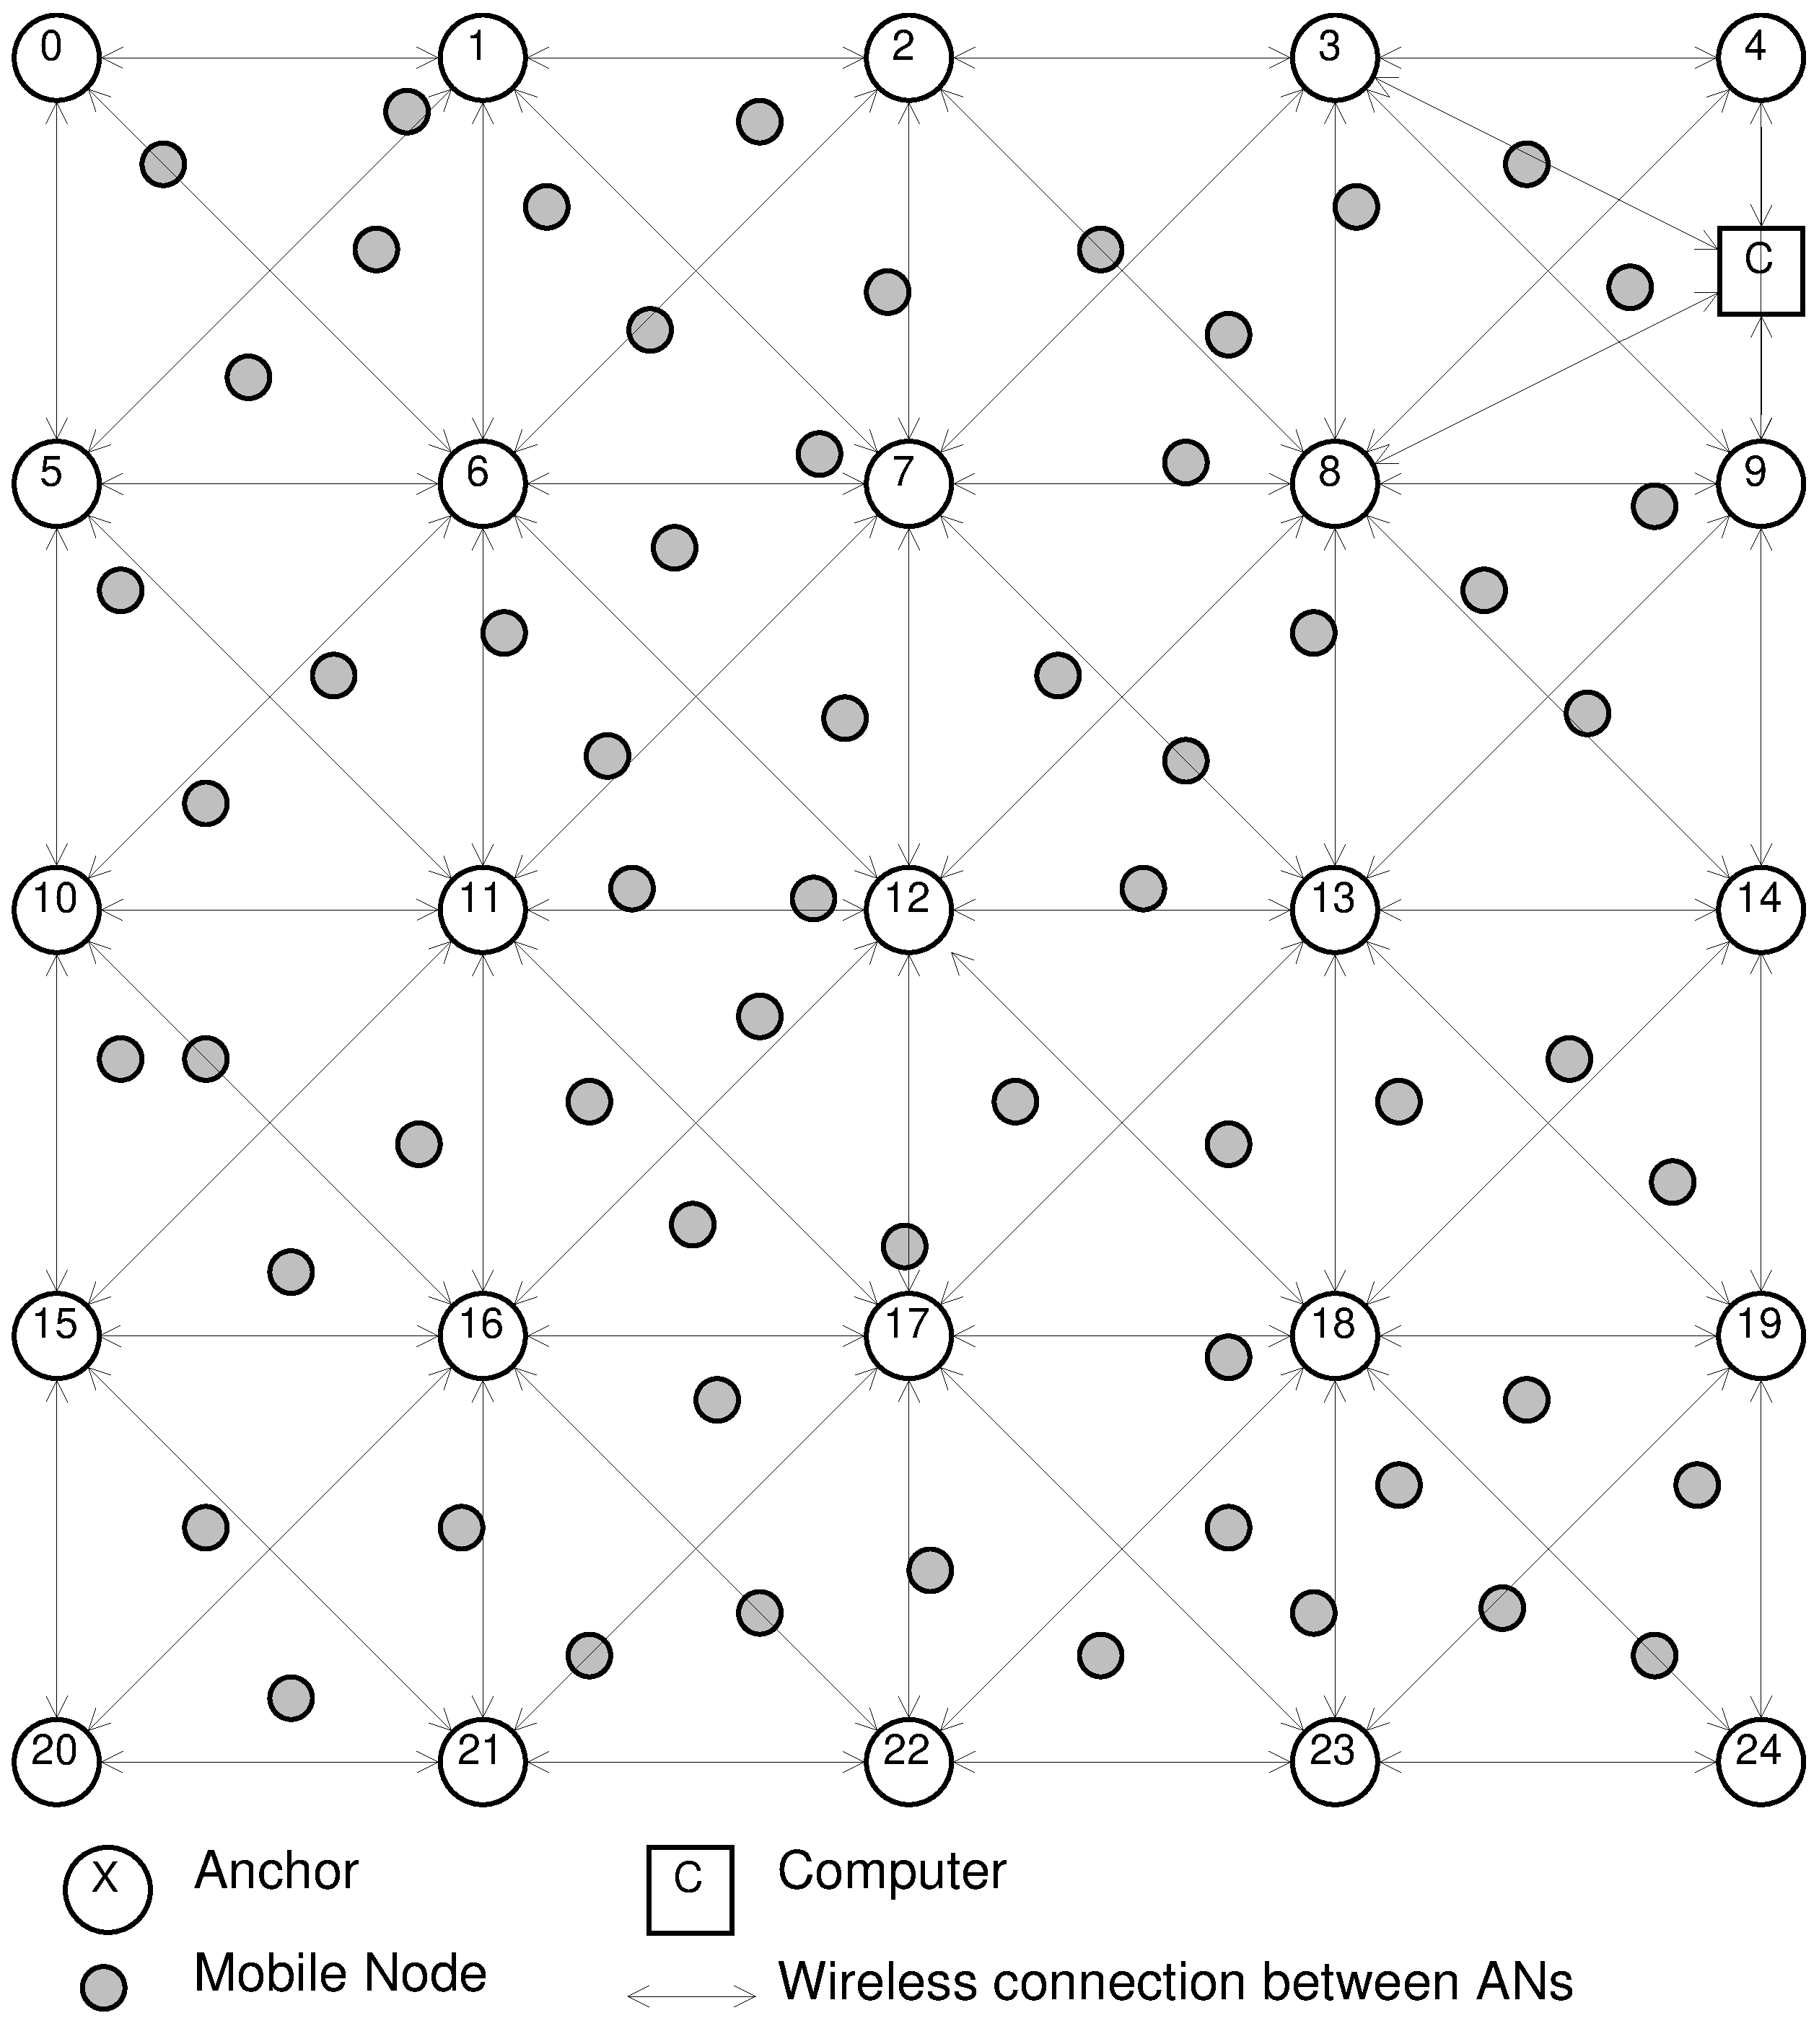
\includegraphics[width=0.5\textwidth]{finalscenario.eps}
 \end{center}
 \caption{Proposed scenario for High Configurable Protocol analysis}
 \label{fig:finalscenario}
\end{figure}

Considering that the period time is 1.5 s, the ComSink Phases are 0.5 s each and that there are $9\cdot3$ slots in each Sync Phase with 
1.5 ms each one of them, the following phase times are obtained:

\begin{verbatim}
    Sync Phases length:     0.0405 s
    Report Phase length:    0.2271 s
    VIP Phase length:       0.1514 s
    ComSink Phases length:  0.5000 s
\end{verbatim}

To force different situations and to be able to check the different \acp{MN} modes, ten configurations are going to be proposed. These 
configurations could be changed just modifying some parameters (explained in Section \ref{sec:ProtocolDescription}: \nameref{sec:ProtocolDescription}). 
Each one of these configurations is going to be simulated during 120 s (80 periods), and repeated 100 times to be able to compensate the error 
produced by the generated random numbers. All graphics in this section will have these configurations on X axis.

The configurations are divided into two groups:

\begin{itemize}
 \item \textbf{Non distributed. }Groups the first five configurations, which are going to be the ones loading the network the most. All of these
configurations are going to have the following parameters in common:
\begin{verbatim}
 activePhases = 1
 inactivePhases = 0
 offsetPhases = 0
 offsetSyncPhases = 0
 reportPhases = 4 
 askFrequency = 2
 offsetReportPhases = 0
 NumberOfBroadcasts = 5
\end{verbatim}
As all the offsets are set to zero, all \acp{MN} will start their functionality at the beginning of the first period, all together at the same
time. This is the reason why this group is called ``non distributed''. As it can be observed, inactive periods are set to 0, this way, all \acp{MN} will 
work every period, loading the network all the time. As \textit{reportPhases} = 4, \acp{MN} Mode 2 and 3 will report only 1 out 4 periods, loading even
more the network during these periods. Note also that the number of broadcast per \ac{MN} Mode 3 and 4 are five. These five configurations are taken as
worst case and will be used to have a worst limit to compare with the other ones.

From this group, and attending to the number of \acp{MN} of each Mode (see Figure \ref{fig:ProtocolPhases}) these 5 configurations are proposed:
\begin{itemize}
 \item[-] \textbf{Config 1}: 15 \acp{MN} Mode 1, 15 \acp{MN} Mode 2, 15 \acp{MN} Mode 3 and 15 \acp{MN} Mode 4.
 \item[-] \textbf{Config 2}: 6 \acp{MN} Mode 1, 6 \acp{MN} Mode 2, 15 \acp{MN} Mode 3 and 33 \acp{MN} Mode 4.
 \item[-] \textbf{Config 3}: 6 \acp{MN} Mode 1, 6 \acp{MN} Mode 2, 33 \acp{MN} Mode 3 and 15 \acp{MN} Mode 4.
 \item[-] \textbf{Config 4}: 33 \acp{MN} Mode 1, 15 \acp{MN} Mode 2, 6 \acp{MN} Mode 3 and 6 \acp{MN} Mode 4.
 \item[-] \textbf{Config 5}: 15 \acp{MN} Mode 1, 33 \acp{MN} Mode 2, 6 \acp{MN} Mode 3 and 6 \acp{MN} Mode 4.
\end{itemize}
 \item \textbf{Distributed. }Groups the last five configurations, which are going to be the ones loading the network the less. All these
configurations are going to have the following parameters in common:
\begin{verbatim}
 activePhases = 2
 inactivePhases = 4
 offsetSyncPhases = 1
 reportPhases = 12
 askFrequency = 2
 NumberOfBroadcasts = 3
\end{verbatim}
This time, it can be seen that both \textit{offsetPhases} and \textit{offsetReportPhases} are not common parameters. This is because they are going to be
used to distribute all the \acp{MN} in the time in a way that $1/3$ of the \acp{MN} will start in period 0, another $1/3$ will start in period 2 and the 
rest $1/3$ will start in period 4. As \textit{activePhases} + \textit{inactivePhases} = 6, \acp{MN} will be perfectly distributed to load the network as 
uniformly as possible. Due to the different kinds of \acp{MN}, the distribution in time will be done equally for every kind of \ac{MN}.

As \textit{reportPhases} = 12, \acp{MN} Mode 2 and 3 will report only 1 out 12 periods, that means they will almost not load the network. Note also that 
the number of broadcast per \ac{MN} Mode 3 and 4 is three instead of five. These five configurations are a possible normal way of loading the network.

From this group, and attending to the number of \acp{MN} of each Mode (see Figure \ref{fig:ProtocolPhases}) these 5 configurations are proposed:
\begin{itemize}
 \item[-] \textbf{Config 6}: 15 \acp{MN} Mode 1, 15 \acp{MN} Mode 2, 15 \acp{MN} Mode 3 and 15 \acp{MN} Mode 4.
 \item[-] \textbf{Config 7}: 6 \acp{MN} Mode 1, 6 \acp{MN} Mode 2, 15 \acp{MN} Mode 3 and 33 \acp{MN} Mode 4.
 \item[-] \textbf{Config 8}: 6 \acp{MN} Mode 1, 6 \acp{MN} Mode 2, 33 \acp{MN} Mode 3 and 15 \acp{MN} Mode 4.
 \item[-] \textbf{Config 9}: 33 \acp{MN} Mode 1, 15 \acp{MN} Mode 2, 6 \acp{MN} Mode 3 and 6 \acp{MN} Mode 4.
 \item[-] \textbf{Config 10}: 15 \acp{MN} Mode 1, 33 \acp{MN} Mode 2, 6 \acp{MN} Mode 3 and 6 \acp{MN} Mode 4.
\end{itemize}
Each of these configurations divide the number of \acp{MN} from each mode by 3, assigning the first third \textit{offsetPhases} = 0 and 
\textit{offsetReportPhases} = 2, the second third \textit{offsetPhases} = 2 and \textit{offsetReportPhases} = 4 and the third
\textit{offsetPhases} = 4 and \textit{offsetReportPhases} = 6. This way all nodes will be equally distributed. That is why this group is called
``Distributed''. 
\end{itemize}

From all the previous times and parameters, it can be obtained that in configurations 1 to 5 the \acp{MN} send the following number of packets during
every simulation depending on the Mode they work:
\begin{itemize}
 \item Each \ac{MN} in Mode 1, sends 80 reports and 0 broadcasts (one report in each period).
 \item Each \ac{MN} in Mode 2, sends 30 reports and 0 broadcasts (20 ask reports + 10 request reports).
 \item Each \ac{MN} in Mode 3, sends 30 reports and 300 broadcasts (during 20 report phases, does not send broadcasts).
 \item Each \ac{MN} in Mode 4, sends 80 reports and 400 broadcasts (one report and five broadcasts in each period).
\end{itemize}
The same could be obtained for configurations 6 to 10:
\begin{itemize}
 \item Each \ac{MN} in Mode 1, sends 22 reports and 0 broadcasts (13 reports + 6 extra reports + 3 requests).
 \item Each \ac{MN} in Mode 2, sends 9 reports and 0 broadcasts (6 extra reports + 3 requests).
 \item Each \ac{MN} in Mode 3, sends 9 reports and 78 broadcasts (three broadcasts each active period).
 \item Each \ac{MN} in Mode 4, sends 22 reports and 78 broadcasts (13 + 6 + 3 reports, three broadcasts each active period).
\end{itemize}

It can be easily seen that the number of sent packets is not the same during the 120 s for the ``non-distributed'' and ``distributed'' case. This 
means that both cases cannot be compared directly. This difference has to be taken into account when comparing both cases in the following 
graphics.

To make possible an easier 
comparison, at the end of the chapter, Config 6 will be named Config A and will be compared with Config B. Config B will have exactly the same
parameters as Config A excepting the offsets. In Config B, \textit{offsetPhases} = 0 and \textit{offsetReportPhases} = 2, this way all nodes are
together in the same active periods, making this way a ``non-distributed'' case to compare to.


As a first orienting result and trying to depict what the following analysis will prove, Table \ref{tab:simulationtimes} shows the times 
the computer took to simulate each one of the configurations. This gives a first idea of the different network loads, meaning more load more simulation
time.

\begin{table}
 \begin{center}
  \begin{tabular}{|l|c|}
   %\noalign{\vspace*{0.5cm}}
   \hline
   Configuration 1 & 7 hours 53 min \\
   \hline
   Configuration 2 & 8 hours 57 min \\
   \hline
   Configuration 3 & 8 hours 35 min \\
   \hline
   Configuration 4 & 6 hours 20 min \\
   \hline
   Configuration 5 & 5 hours 55 min \\
   \hline
   Configuration 6 & 5 hours 14 min \\
   \hline
   Configuration 7 & 6 hours 26 min \\
   \hline
   Configuration 8 & 6 hours 12 min \\
   \hline
   Configuration 9 & 3 hours 16 min \\
   \hline
   Configuration 10 & 2 hours 59 min \\
   \hline
  \end{tabular}
  \caption{Simulation times depending on Configuration}
  \label{tab:simulationtimes}
 \end{center}
\end{table}

\subsection{Traffic in the network}

To give an idea of the traffic in the network for the different configurations, \acp{AN} must be studied. All reports or broadcasts generated by the
\acp{MN} are later on retransmitted to the coordinator (in all cases a centralized schema was used). \acp{AN} are the ones in charge of distributing these
information as well as routing the information coming from and to the computer. This is why ComSink phases are going to be the most loaded
phases and therefore their case the most interesting to be studied.

\begin{figure}[ht]
 \begin{center}
  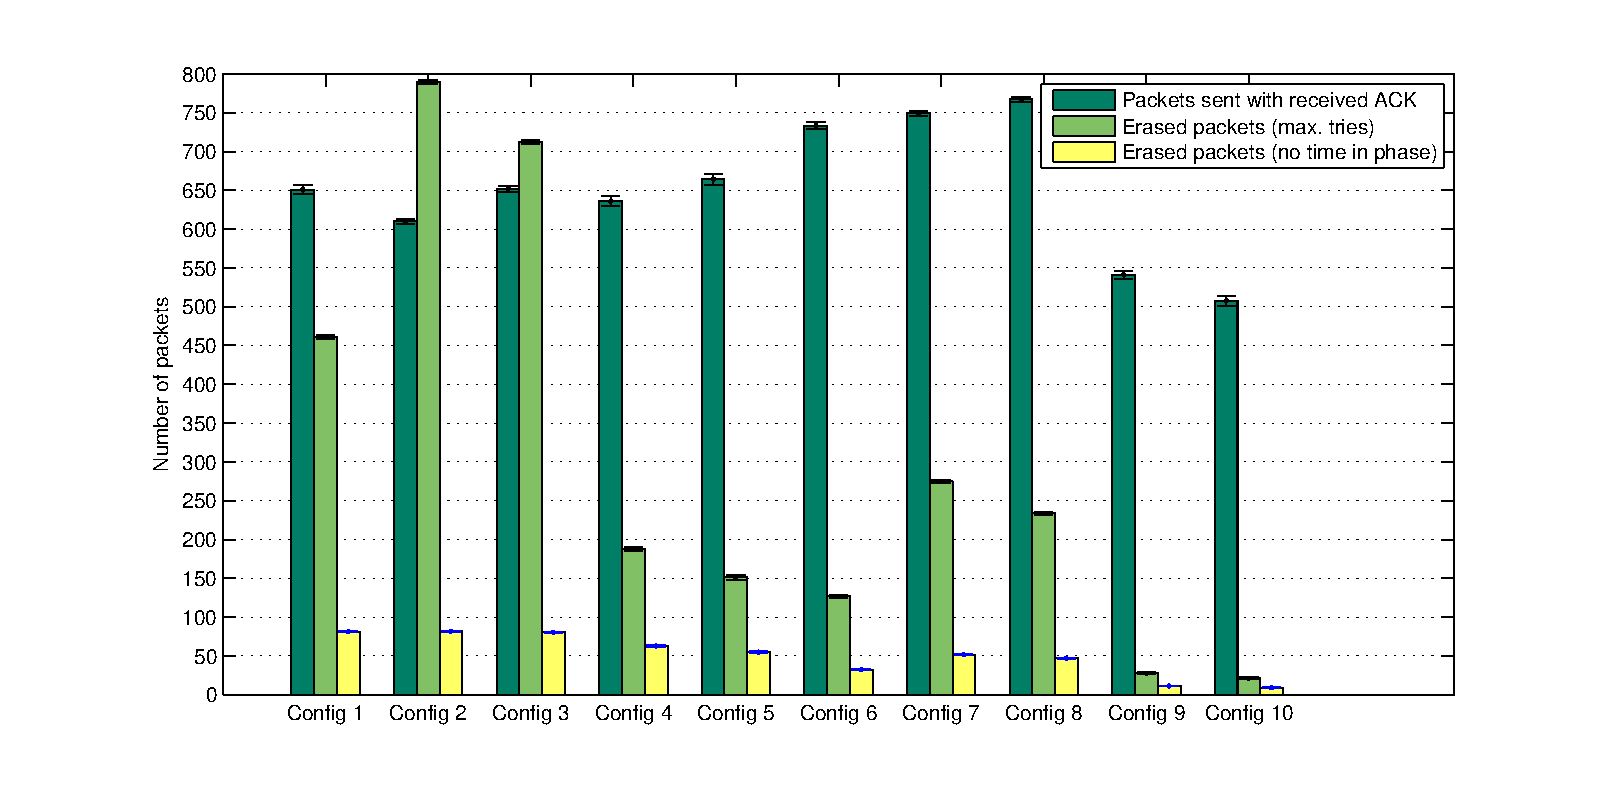
\includegraphics[width=1\textwidth]{packetsSentErasedNoTimeAN.eps}
 \end{center}
 \caption{Traffic statistics for the \acp{AN}}
 \label{fig:packetsSentErasedNoTimeAN}
\end{figure}

In \textbf{Figure \ref{fig:packetsSentErasedNoTimeAN}}. Erased packets due to maximum number of retransmissions are more numerous in non-distributed 
configurations than in the distributed ones. This is because in non-distributed ones, all \acp{MN} transmit in every period, generating much more traffic
than in distributed ones. This makes the \acp{AN} traffic in ComSink Phases bigger than what the channel can absorb, eliminating therefore many packets 
due to the high number of collisions they had.

When a \ac{MN} sends a broadcast, unlike for reports, this packet reaches more than one \ac{AN} generating X times the traffic of a report (X = number of \acp{AN}
who received the broadcast). This is the reason why in the figure it can be observed that for configurations 2 and 3 or 7 and 8 where the number of 
\acp{MN} who broadcast are increased, the number of erased packets due to maximum number of retransmissions is increased respecting configurations
1, 4 and 5 or 6, 9 and 10.

In the case of configurations 1, 2 and 3, there are many erased packets, some times even more than correctly sent packets. This makes possible 
for configurations 6, 7 and 8, as the number of collisions is smaller, to achieve a bigger number of successfully delivered packets, even 
when for distributed configurations, the total number of sent packets by the \acp{MN} is smaller.

Erased packets due to a lack of time in the phase, are the erased packets when the end of ComSink Phases is approaching (10 ms of guard time is left
before the end of the phase). When a change of phase approaches, all scheduled packets to be sent, must be deleted or postponed, otherwise they will be 
transmitted during the next Sync Phase, provoking non desired collisions.

Like for the deleted packets due to maximum number of retransmissions case, erased packets due to a lack of time in the phase are more numerous in the 
non-distributed case. In configurations 1, 2 and 3, it can be seen how this value reaches a maximum, being the same in the three cases. If this 
is compared with the distributed case, as this value does not saturate, the logic behavior can be seen. For configuration 1, the deleted packets 
are less than for the configurations where there are more \acp{MN} in Modes 3 and 4 and therefore more broadcasts. This saturation value is reached 
because there are so many collisions, that the \acp{AN} do not receive further packets to be routed. When the guard time approaches, the \acp{AN} only have 
to send their own generated packets scheduled to be sent some time before, and the ones to be routed which managed to be delivered with all the 
network saturation.

\subsection{Transmission efficiency in \acp{MN}}

In this sub-section an idea of the efficiency of a \ac{MN}'s transmission is given. This will be done by analyzing the average number of \ac{CSMA/CA}
Backoffs and their average time before a transmission gets to be done. The number of retries done due to a lack of \ac{ACK}, will be also analyzed.

\begin{figure}[ht]
 \begin{center}
  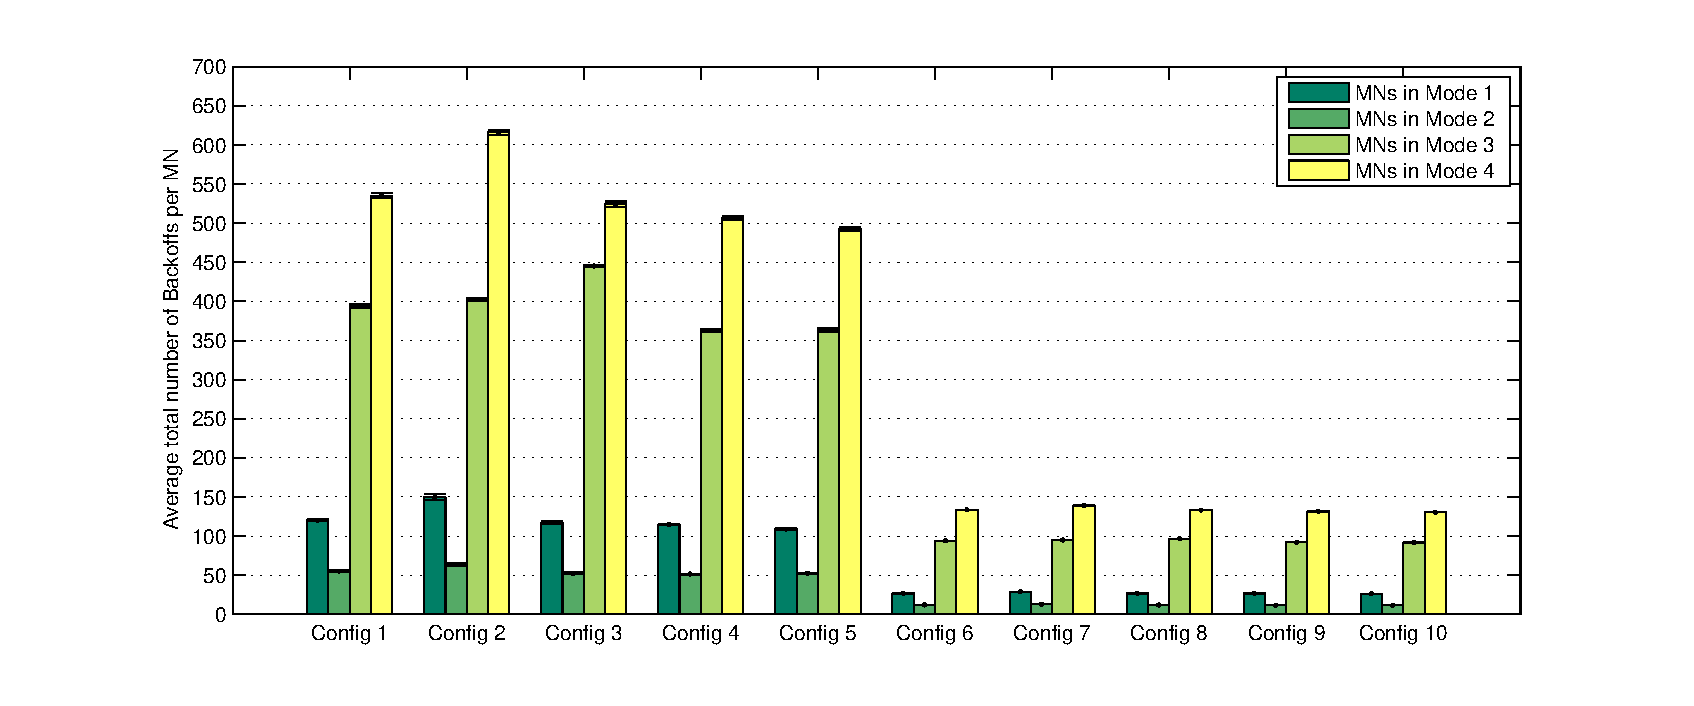
\includegraphics[width=1\textwidth]{BackoffNumberInMN.eps}
 \end{center}
 \caption{Average Backoff number for different modes and configurations}
 \label{fig:BackoffNumberInMN}
\end{figure}

In \textbf{Figure \ref{fig:BackoffNumberInMN}} can be easily seen how for the configurations 1 to 5, when the network is more loaded, the number of 
average Backoffs is bigger than for the normal case in configurations 6 to 10. This is due to the total sent packets number.

It is in general seen that \acp{MN} in modes 3 and 4, which send broadcasts, have a bigger number of Backoffs than \acp{MN} in modes 1 and 2. The same 
happens between \acp{MN} in mode 1, which sends more reports than \acp{MN} in mode 2. As each packet needs at least one Backoff regardless of the type of 
packet, this difference is caused by the total number of sent packets by each \ac{MN} in each mode. This difference is bigger for the configurations 1 
to 5 because, as the number of packets sent to channel is bigger, the \acp{MN} find more often the channel busy and therefore they need at least another Backoff
period.

In configurations 6 to 10 can be seen that all values are very similar independently of the configuration. As all packets to be transmitted have at least
one Backoff period, these constant values are showing the minimum number of Backoffs. As these configurations almost do not load the network, these values 
depend basically on the number of packets to be sent.

In configuration 2, for example, it can be observed how as the number of \acp{MN} in mode 4 was arisen, the Report Phase is more loaded, and average
Backoff periods needed by \acp{MN} in modes 1, 2 and 4 grows in comparison with configuration 1 (equilibrated configuration), specially for \acp{MN} in
mode 4. \acp{MN} in mode 3 do not get affected so much because they have their own phase to transmit.

In configurations 4 and 5, when the number of \acp{MN} who transmit only reports is arisen, the average number of Backoff periods goes down in general,
this is because reports do not charge the network like broadcasts do.

It is interesting also to see that for configuration 3, where \acp{MN} in mode 3 are predominant, almost only \acp{MN} in mode 3 are affected. This is
because they have their own phase (\ac{VIP} Phase) to transmit, and their transmissions do not affect the other modes.

\begin{figure}[ht]
 \begin{center}
  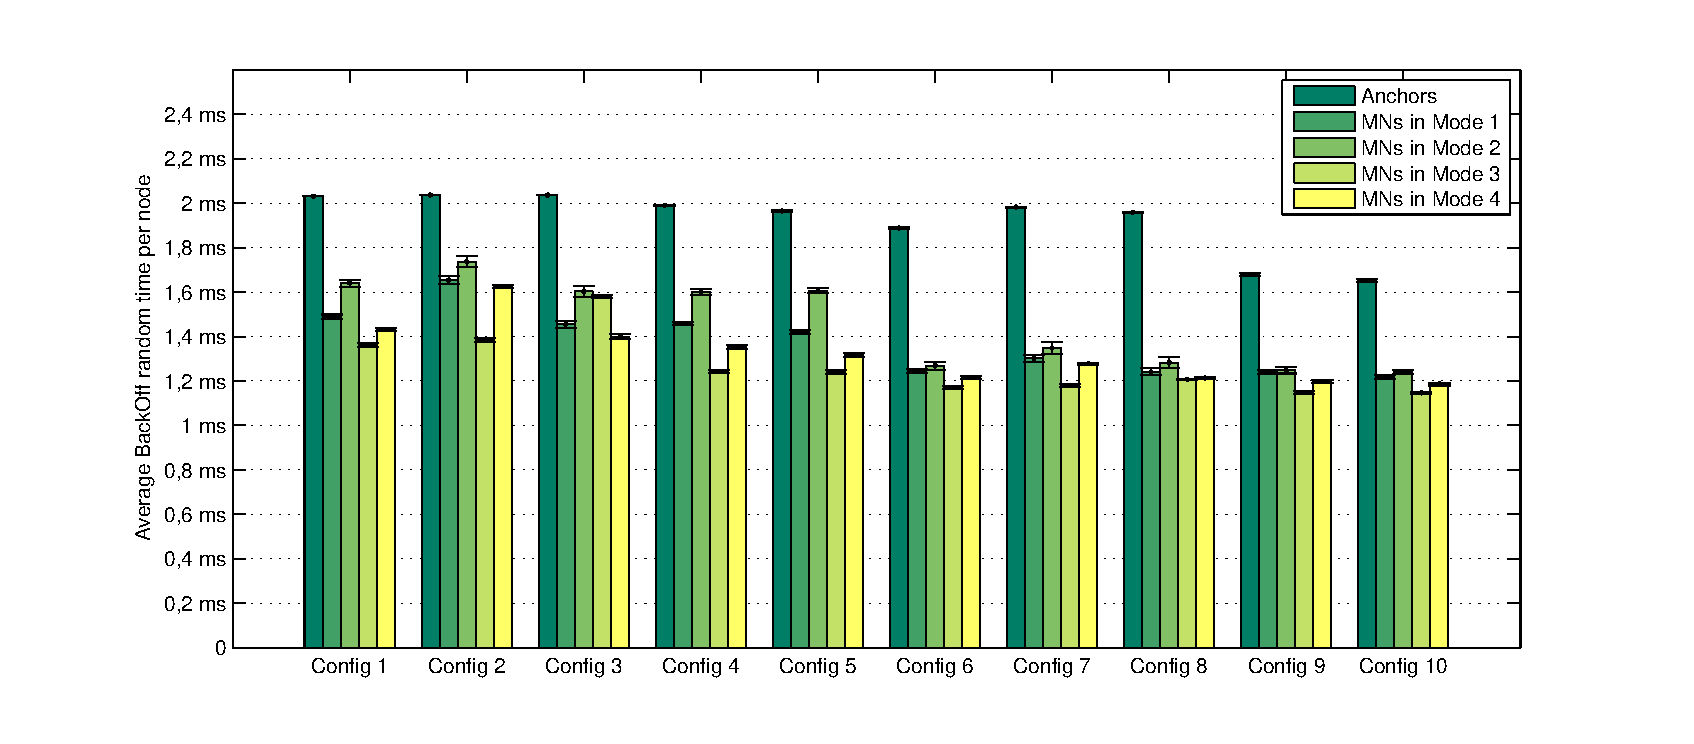
\includegraphics[width=1\textwidth]{averageBackoffTimeANandMN.eps}
 \end{center}
 \caption{Average Backoff times for different nodes and configurations}
 \label{fig:averageBackoffTimeANandMN}
\end{figure}

For a good analysis of \textbf{Figure \ref{fig:averageBackoffTimeANandMN}}, it needs to be observed that according to (\ref{mat:backoffexpression}),
the first Backoff time in average is 1.12 ms.
\begin{equation}
  rand(0;  2^3-1)\cdot aUnitBackoffPeriod = rand(0; 2^3-1)\cdot 320\mu s\ \cite{IEEE802.15.4-2006}
  \label{mat:backoffexpression}
\end{equation}
With this data in mind, it can be seen in the figure that, excepting for the \acp{AN} where (as it was already said in previous sub-section) the 
number of deletions and therefore retransmissions is high, all average Backoff times are not much bigger than this minimum average value. That shows that for
all configurations, even from 1 to 5 where average Backoff time is a little bit bigger, the number of Backoffs due to a busy channel is not that high and 
neither the average Backoff time. The data from this figure, together with the one from Figure \ref{fig:BackoffNumberInMN} gives
also an idea of the idle listening necessary for each mode to be able to transmit a packet.

From the figure can also be extracted that in configuration 2, as the network load grows, also does the average Backoff time for \acp{MN} in modes 1, 2 
and 4. \acp{MN} in mode 3 do not see their average Backoff time increased because, like it was already said, they transmit in their own phase. For this
reason can be also seen that in configuration 3, only average Backoff time for \acp{MN} in mode 3 gets considerably increased.

Configurations 4 and 5 show how, decreasing the number of broadcasts in Report Phase (less \acp{MN} in mode 4), as the number of packets in the channel
gets reduced, the average Backoff time for all modes gets also reduced. This is because whenever a \ac{MN} wants to transmit a report, it is easier to 
find the channel free.

Last but not least, there is a strange detail in the figure. Why if \acp{MN} in mode 2 are the ones sending the less packets to the network, is their 
average Backoff time the biggest in all configurations? This happens because the way the network is configured, all extra report periods, match up in time
with other active periods, in configurations 1 to 5 all periods are active for all \acp{MN} and in configurations 6 to 10 all periods are active for 
some \ac{MN} (they are distributed in time). This means that, as \acp{MN} in mode 2, transmit their packets only in extra report periods, they are going to 
find always a more loaded network and therefore its average Backoff time will be bigger. The other \acp{MN} in modes 1, 3 and 4 are transmitting  
also during the loaded extra report periods and are getting high Backoff time values, but, as they transmit also in calmer periods, their average Backoff time will be reduced.

\begin{figure}[ht]
 \begin{center}
  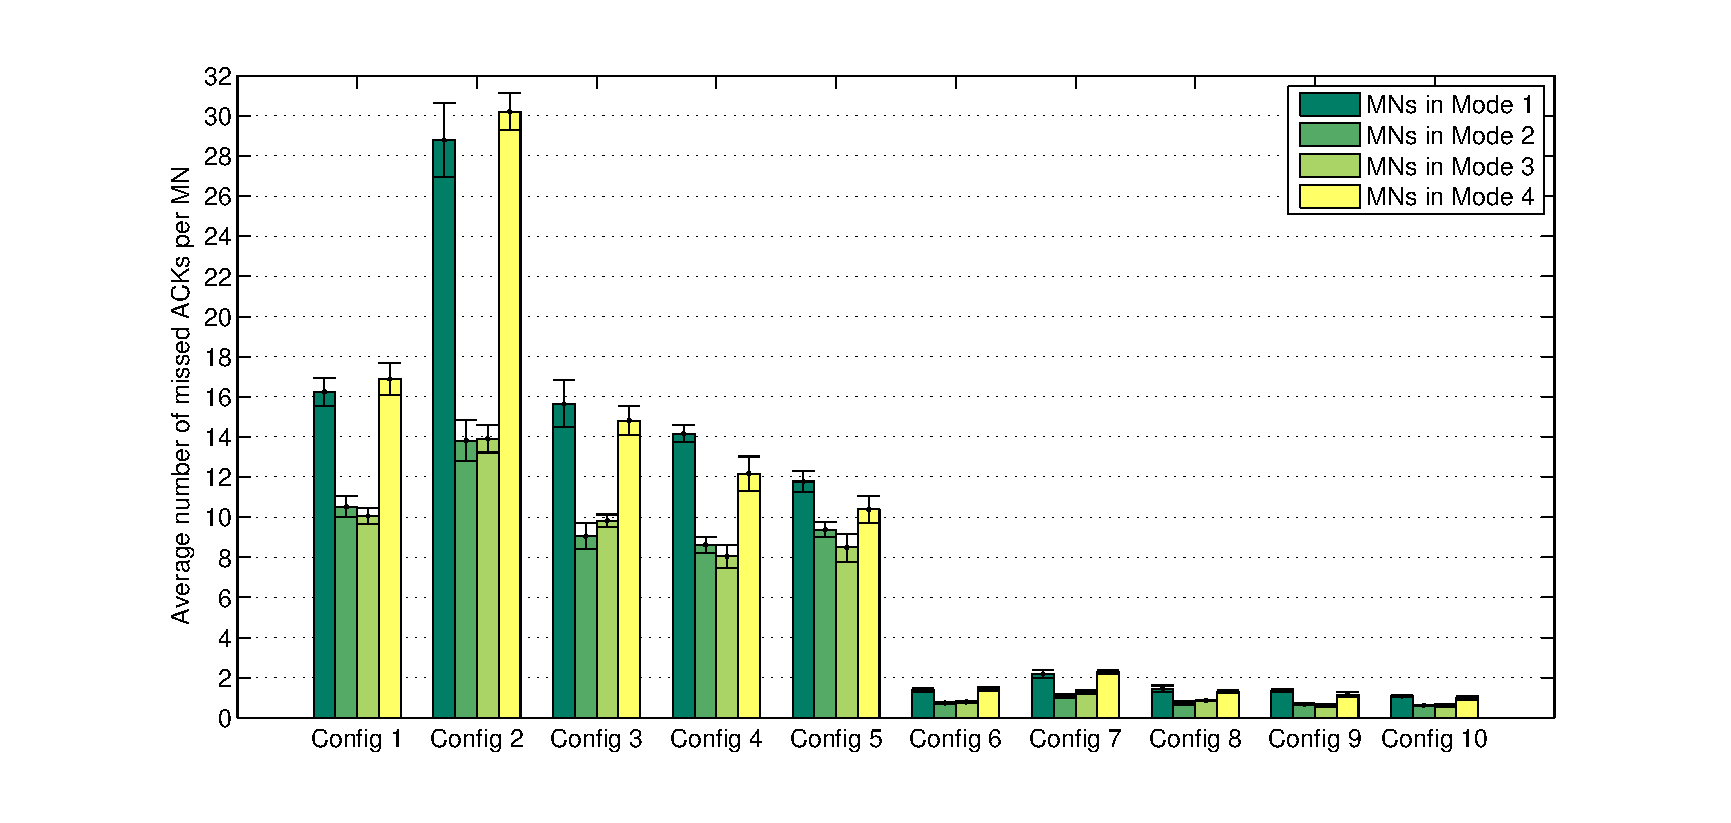
\includegraphics[width=1\textwidth]{nbMissedACKMN.eps}
 \end{center}
 \caption{Average number of report retransmissions due to the lack of ACK}
 \label{fig:nbMissedACKMN}
\end{figure}

Reports are the only packets sent by \acp{MN} where an \ac{ACK} is answered to confirm the correct packet delivery. Reports are just sent during the
Report Phase and the lack of \ac{ACK} clearly means a collision. That is why \textbf{Figure \ref{fig:nbMissedACKMN}} shows how loaded the Report Phase is
for the different configurations and how the different \acp{MN} modes get affected. As in previous figures the influence of network load was not easy to
see, in this figure it can be easily seen that for configurations 1 to 5 the number of collions is much bigger than for configurations 6 to 10.

As the lack of \ac{ACK} affects only the reports, it can be also seen how \acp{MN} in modes 1 and 4 and \acp{MN} in modes 2 and 3 get in all cases similar
values as they send almost the same number of reports.

As in configuration 2, there is a bigger number of broadcasts loading the Report Phase with much more traffic, the number of retransmissions due to 
the lack of \ac{ACK} gets much bigger.

\paragraph{Conclusion.} The number of Backoffs together with the number of retransmitted packets due to the lack of ACK, show us that \acp{MN} transmissions 
are quite efficient for these configurations, at least compared with \acp{AN} transmissions. From these results can directly be extracted that, while 
Report and VIP Phase times are good enough, the ComSink phases times should be bigger for some of the configurations.

\subsection{Energy consumption in \acp{MN}}

As it was already said during this work, all \acp{MN} have different working states: sleep all, sleep but $\mu C$ working, idle, transmission and 
reception. Each of these states has a different energy consumption (Table \ref{tab:NodeEnergyConsumption}), and transitions between states take 
different times (Table \ref{tab:NodeTiming}). During the simulation, all \acp{MN} changed their states as explained in Section 
\ref{sec:frameworkdevelopment}: \nameref{sec:frameworkdevelopment}. The times in the different states and in all possible transitions between states were stored
during the 120 s of simulation. These times multiplied by the energy consumed for each case and added together, result in \textbf{Figure \ref{fig:energyConsumptionPerMN}}.

\begin{figure}[ht]
 \begin{center}
  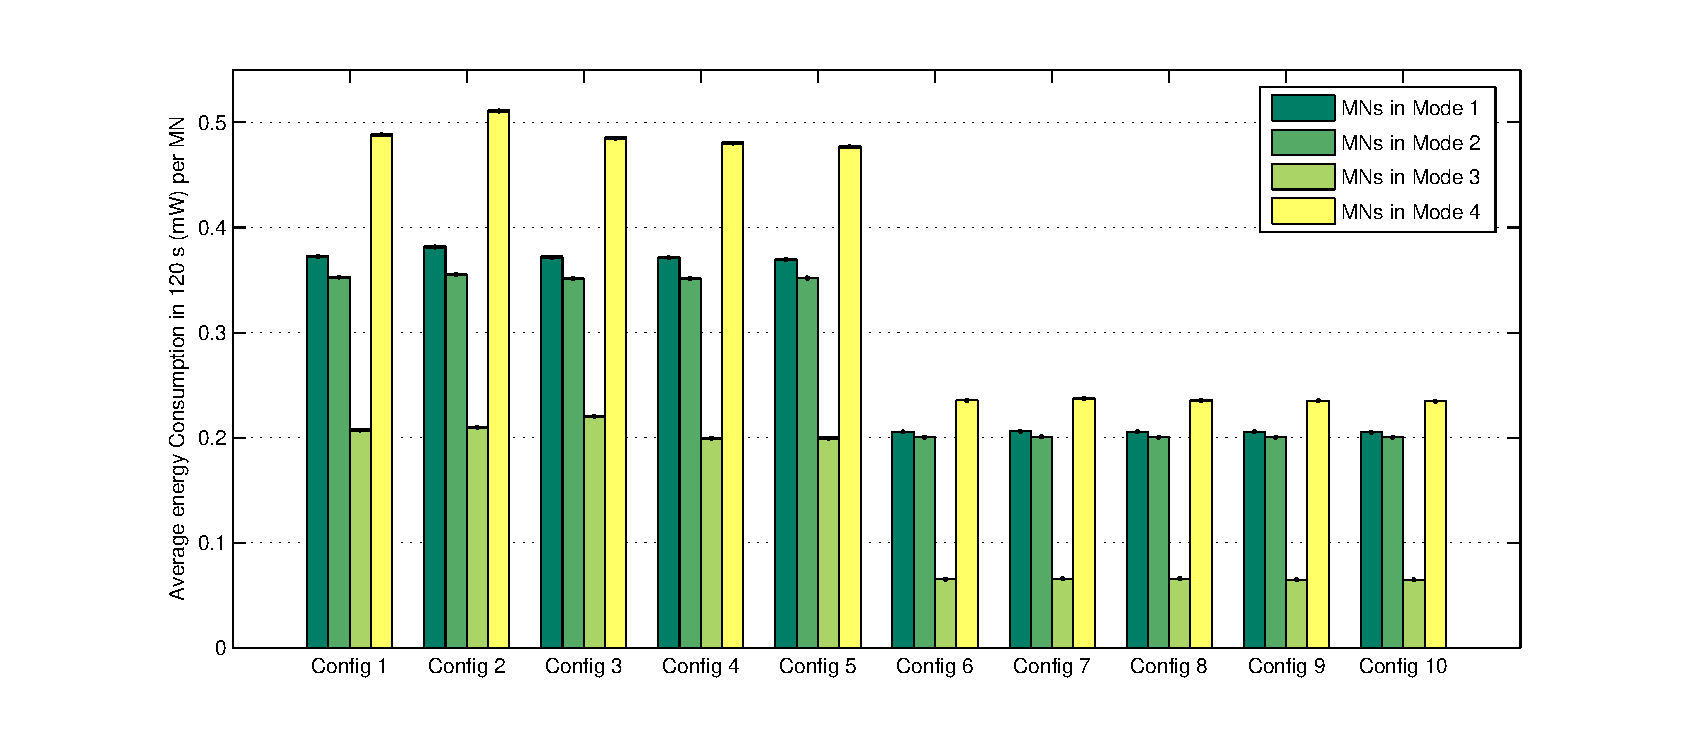
\includegraphics[width=1\textwidth]{energyConsumptionPerMN.eps}
 \end{center}
 \caption{Average energy consumed by any \ac{MN} in 120 s (mW)}
 \label{fig:energyConsumptionPerMN}
\end{figure}

Figure shows how for configurations with the same parameters (configurations 1 to 5 and 6 to 10), the consumed energy values stay approximately
constant independently of the network charge. This independence, means that \acp{MN} consume most of the energy when listening during Sync Phases and 
when transmitting, but not in retransmissions due collisions. This good performance of \acp{MN} during Report and \ac{VIP} phases was already seen
in the previous sub-section and is also confirmed here. 

In configuration 3, a light growth in energy can be appreciated for \acp{MN} in mode 3. This is caused by the increment of broadcasts number to share the 
\ac{VIP} Phase. Anyway, this increment is not that big. This shows that even this mode, with a shorter in time \ac{VIP} Phase, is not very much affected
by collisions. In configuration 8, this effect is even not appreciable because instead of 5 broadcasts per \ac{MN} only 3 are sent, and also because
\acp{MN} are distributed in time, being possible to find transmitting at the same period only $1/3$ of the \acp{MN} in mode 3.

In configuration 2, a light growth in energy for \acp{MN} in mode 4 can be also appreciated. The reason is exactly the same as for \acp{MN} in mode 3.

Another important aspect extracted from the figure is that although \acp{MN} in mode 1 transmit more reports that \acp{MN} in mode 2, their energy
consumptions are almost the same. This means that for \acp{MN} in modes 1 and 2, which do not transmit broadcasts, the biggest part of the consumed energy,
comes from listening to the Sync Phases.

A last reflexion involves \acp{MN} in mode 1 and 4. Their behavior is very similar, finding as only difference that \acp{MN} in mode 4 apart from 
listening to Sync Phases and transmitting reports, transmit also broadcasts. This way it can be noted that the difference in energy consumed for both
modes, represents the energy consumed transmitting the broadcasts. To assert this affirmation, it can be seen that for configurations 1 to 5, where
5 broadcasts per \ac{MN} in mode 4 are sent, the energy consumption difference between \acp{MN} in mode 1 and in mode 4 is bigger than for configurations
6 to 10 where the number of broadcasts per \ac{MN} in mode 4 is just 3.

\subsection{Fair comparison}

As it was said, to be able to easily compare a ``distributed'' configuration and a ``non-distributed'' one, they must transmit in overall the same
number of packets during the same time. To achieve this, the already introduced, Configurations A and B were created.

A first comparison, in this case about the \acp{MN}, can be seen in \textbf{Figure \ref{fig:MNsAverageValuesin120s}}. Comparing both
configuration values and looking at the previous sub-sections figures, it can be seen that in this case, when the total sent packets are the 
same, the values for ``distributed`` and ``non-distributed`` cases, do not differ so much like before. Anyway, higher values can be observed 
for Configuration B than for A. This is because, as in Configuration B all packets concentrate in the same periods, the network load is 
bigger causing more collisions in Configuration B than in A.

\begin{figure}[ht]
 \begin{center}
  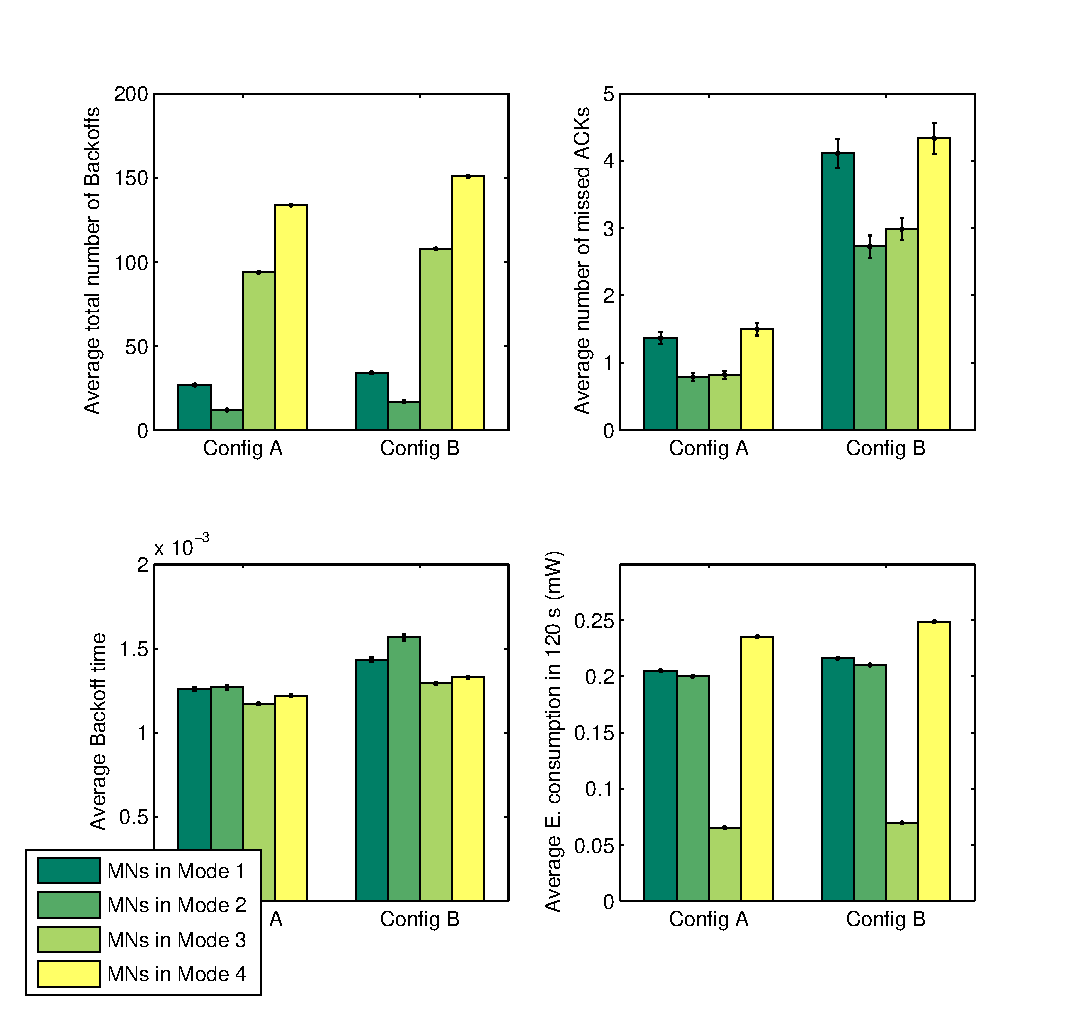
\includegraphics[width=0.9\textwidth]{MNsAverageValuesin120s.eps}
 \end{center}
 \caption{\acp{MN} average values comparison}
 \label{fig:MNsAverageValuesin120s}
\end{figure}

For the previous figure, almost no difference between configurations could be seen. This is because, as it was already said, the performance
during the Report and \ac{VIP} Phases is really good. When comparing the \acp{AN} performance, a more different behavior can be seen. 
\textbf{Figure \ref{fig:ANsConparison}} shows these differences. 

\begin{figure}[ht]
 \begin{center}
  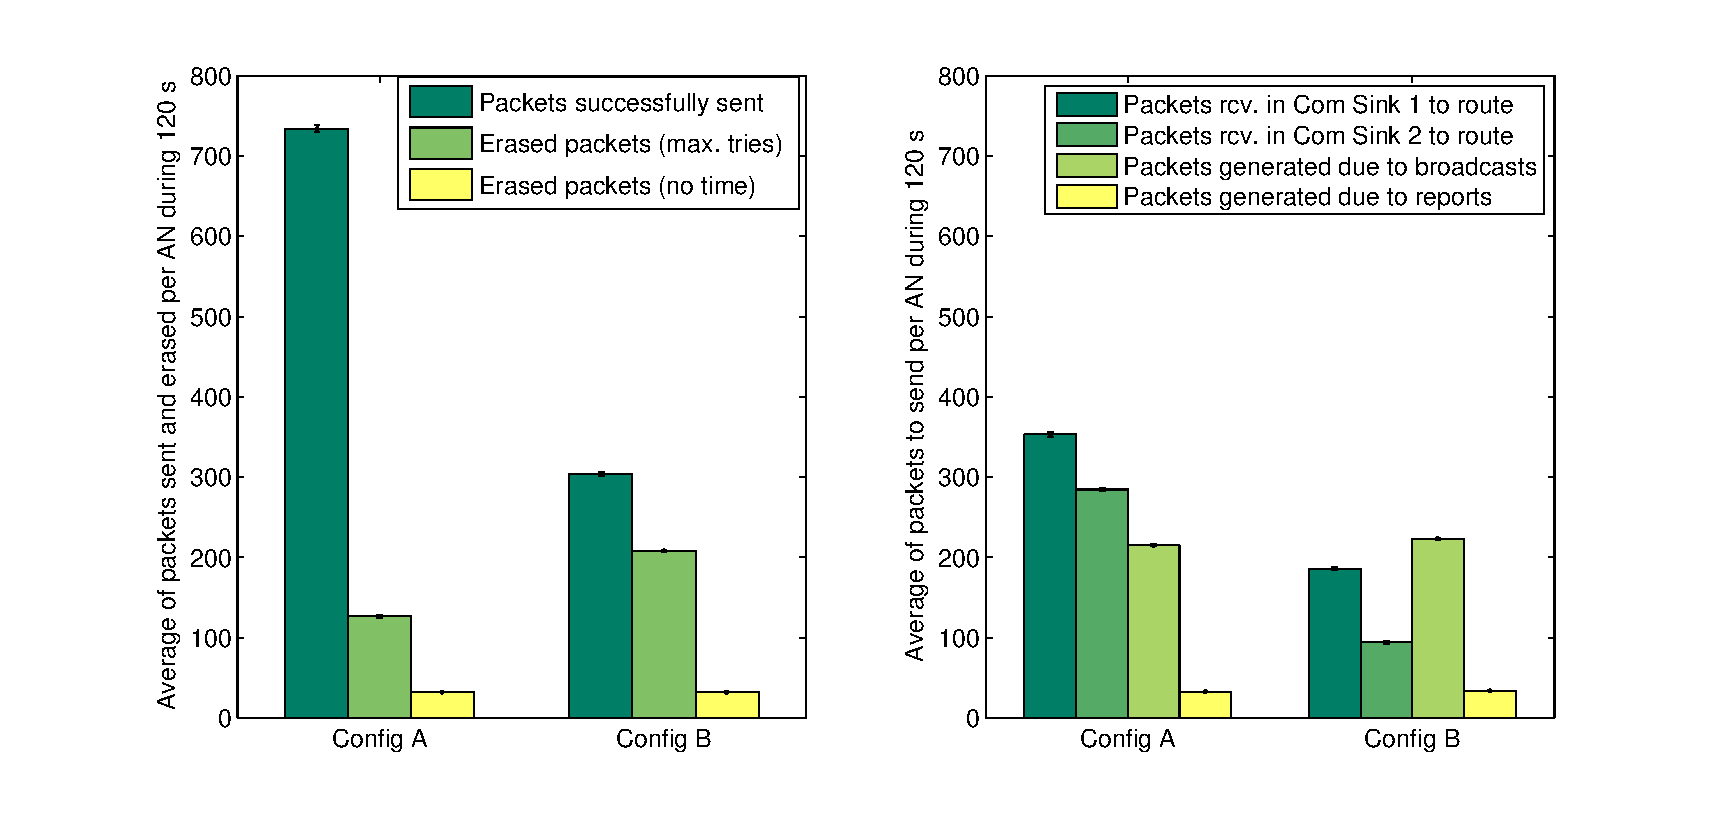
\includegraphics[width=0.9\textwidth]{ANsConparison.eps}
 \end{center}
 \caption{\acp{AN} average values comparison}
 \label{fig:ANsConparison}
\end{figure}

As the network traffic is more concentrated for Configuration B than for A, in the graphic on the left can be seen how the number of erased 
packets due to maximum number of retransmissions is higher, and therefore the number of successfully transmitted packets is smaller. But the 
strange aspect is, why the addition of successfully sent packets, and all the erased packets is not the same for both configurations if the 
number of generated packets in the \acp{MN} is the same? 

Previous question gets explained in the graphic on the right. In this graphic can be seen how the total number of generated packets from an 
\ac{AN}, due to generated packets in \acp{MN} (broadcasts and reports), is the same for both configurations. The only difference can be 
found in the packets an \ac{AN} routes to or from the computer. In this case the number for Configuration B is much smaller. But, how can 
the difference be so high, if the difference in erased packets is not? This is because every time a route packet is deleted, this does not only
mean that a packet less will be transmitted, but also that in the following hops until computer (ComSink 1) or until selected \ac{AN} (ComSink
2) new packets will not even be created. According to the routing diagram showed in Figure \ref{fig:routetree} (page \pageref{fig:routetree}), it is
obtained that a packet from an \ac{AN} has to hop an average of 2.88 steps to reach its destination. Therefore, a deleted 
routed packet means reducing in average the generated packets by 2.88. This ratio can prove the difference between erased packets
and the number of generated packets between configurations.


\chapter{Conclusion and future work}
\label{chap:conclusionsandfuture}

Mirar conclusiones del paper.

Comentar que los slots han resultado se mejores y por ello se usan en el framework final

Comentar que nodo 2 puede ser bueno para no cargar la red, que lo que mas consume es escuchar y por ello node 3 consume el que menos y por tanto
hay que usarlos para bajo consumo. 


Look for the best parameters in the simulation.

Change node configuration.

Results Shows that distribution in time is really important.

En las fases com sink se aprecia la sobre carga de la red, pero en los estudios de los nodos moviles, se aprecia un buen funcionamiento y la diferencia
de configs sin distribuir y distribuidas es debida en su mayoria al numero total de paquetes mandados.

Move the nodes.

Comment how long the nodes would last with this protocol.

\bibliographystyle{unsrt}
\bibliography{bib}

\appendix
\chapter{Source code first contact}
\label{chap:installation}

\section{Git Introduction}

\section{OmNet++, \ac{MiXiM} and my code}


% Pages with extra content of the document
\appendix

\end{document}